
                                                                 %%%%%%%%%%%%%%%%%%%%%%%%%%%%%%%%%%%%%%%%%%%%%%%%%%%%%%%%%%%%%
% Compile settings
%%%%%%%%%%%%%%%%%%%%%%%%%%%%%%%%%%%%%%%%%%%%%%%%%%%%%%%%%%%%%

% Make preprint? For languish check.
\def\makepreprint{n}

% Include the papers?
\def\includepapers{n}

% Final papersize B5 (nicer 'book'-format)? If no, it will be A4.
\def\finalsizeB5{n}

% Make digital version(i.e. with coloured links)? If not, the links will be black so it looks nice when printed.
\def\digitalversion{y}


%%%%%%%%%%%%%%%%%%%%%%%%%%%%%%



%%%%%%%%%%%%%%%%%%%%%%%%%%%%%%%%%%%%%%%%%%%%%%%%%%%%%%%%%%%%%

% Document class
\if \makepreprint y
    \documentclass[a4paper,showtrims,11pt,draft]{memoir}
\else 
		\if \finalsizeB5 y
				\documentclass[a4paper,showtrims,11pt]{memoir}'
		\else
				\documentclass[a4paper,11pt]{memoir} 
		\fi
\fi


 %Format settings
%%%%%%%%%%%%%%%%%%%%%%%%%%%%%%%%%%%%%%%%%%%%%%%%%%%%%%%%%%%%%%%%%%%%%%%%%%%
% Package loading that allows compilation to pdf either with dvips+ps2pdf or pdflatex.
% For pdf figures must be in format pdf (or jpg). This can be done with epstopdf (%f in (*.eps) do epstopdf %f)
% For pdf via dvi and ps figures must be in format eps.

%\newif\ifpdf\ifx\pdfoutput\undefined\pdffalse\else\pdfoutput=1\pdftrue\fi% Latex mode i.e. \pdfoutput is only defined compiling with pdflatex
%Above row is commented since this declaration is already done in the memoir class
\ifpdf
  \usepackage[pdftex]{graphicx}
  %\usepackage{epstopdf} % This does not work on windows.
  \usepackage[pdftex,dvipsnames,usenames]{color} % This package allows for use of colors
  \DeclareGraphicsExtensions{.pdf,.png}
  \pdfadjustspacing=1  % Use LaTeX like spacing and not pdflatex layout algorithm
  %\usepackage[pdftex]{thumbpdf}
  \usepackage[protrusion={true, compatibility},expansion={true, compatibility}]{microtype} % Margin kerning i.e. prettier margins
\else
  \usepackage{graphicx}
  \usepackage[dvips,dvipsnames,usenames]{color} % This package allows for use of colors
  %\usepackage[ps2pdf]{thumbpdf}
  \DeclareGraphicsExtensions{.eps}
\fi

%R. Géneaux - Fixes the "too many alphabet" errors :
\newcommand\hmmax{0}
\newcommand\bmmax{0}


%--------------------------------------------------------------------------------%
%\usepackage[pagebackref]{hyperref}%A Camper for bak paging the reference
%\usepackage{utopia}					% Utopia font as default roman
\usepackage{mathpazo}				% Zapf Palatino font as default roman. Math in Palatino where possible
\usepackage{amsmath,amssymb,MnSymbol} %
%\usepackage{nomencl}         % The nomenclature package can be used to generate and format a
                             % nomenclature using MakeIndex. I use to make a List of Symbols
\usepackage{braket}          % braket: Macros for Dirac bra-ket <|> notation and sets {|}'
\usepackage{array}           % Extends the implementation of array- and tabular-enviroments
%\usepackage[numbers,square,comma,sort&compress]{natbib}
\usepackage[authoryear,square,comma,sort&compress]{natbib}
\usepackage{systeme}
%\usepackage[authoryear,sort,colon,square]{natbib}
\usepackage{ifthen}
\usepackage{calc}
\usepackage{url}
 \usepackage{eurosym,skull}
\usepackage{amsmath,amssymb,graphicx,stmaryrd}% Installé par Antoine pour \sslash 
\usepackage{MnSymbol}
\usepackage{picins}
\usepackage{bm}							%gives \bm{xx} command in math mode - more effective way to use bold variables
%\usepackage{color}
%\usepackage{setspace}
%\usepackage{textcomp}        % Defines for example dregrees celcius symbol
%\usepackage{siunitx}         % The SIunitx package provides macros to type numbers and
                             		% units in a consistent way according to SI requirements.
%\usepackage{ulem}            % Allows line through text, \sout{},  under line, \uline{}
                             % wavy under line, \uwave{}, double under line, \uuline{}
                             % text market with slashes, \xout{}
%\normalem                    % Stops ulem of taking over the \emph{} command
\usepackage[utf8]{inputenc}
\usepackage[T1]{fontenc}%A Camper problème d'accents dans l'hyphénation
\usepackage[french]{babel}
\usepackage{icomma} 
\usepackage[table]{xcolor}% http://ctan.org/pkg/xcolor
\DeclareUnicodeCharacter{00A0}{ }
\DeclareUnicodeCharacter{00A0}{ }
%
\ifpdf
  %\usepackage[pagebackref]{hyperref}
	\usepackage[backref=page]{hyperref}
  %\usepackage[pdftex]{hyperref}
\else
  \usepackage[ps2pdf]{hyperref}
  %\usepackage[hypertex]{hyperref}  %% Gives hyperreferenses in the dvi file.
  % \hypersetup{pdffitwindow=false}
\fi
%\usepackage{hypernat} %% Makes the hyperref and natbib packages work together i.e. [1-3] works
%\usepackage{memoir/hypernat} %% Makes the hyperref and natbib packages work together i.e. [1-3] works
\usepackage{memhfixc} %% The memhfixc package provides hyperref related temporary
                      %% fixes and extensions for version v1.3a of the memoir class.

%R. Géneaux
\usepackage{siunitx} %macros for proper typeset SI units
\sisetup{
list-final-separator = { et }
}
\usepackage{titlesec}
\usepackage{import} %The import package allows to use latex+pdf from inkscape when files are in a different folder
\usepackage{transparent} %Handles transparency when importing svg files
\usepackage[all]{xy} %Used for drawings with arrows

\titleformat{\paragraph}
{\normalfont\normalsize\bfseries}{\theparagraph}{1em}{}
\titlespacing*{\paragraph}
{0pt}{3.25ex plus 1ex minus .2ex}{1.5ex plus .2ex}

%RGéneaux - reduce space after subsubsection
\titlespacing{\subsubsection}{0pt}{\parskip}{-5pt}

% Appearance
\hypersetup{
%bookmarks = true,
bookmarksnumbered = true,
breaklinks = true
}

\ifthenelse{\equal{\digitalversion}{y}}
{
  \hypersetup{
  colorlinks = true,
  linkcolor = blue,
  citecolor = red
  }
}
{
  \hypersetup{
  colorlinks = true,
  linkcolor = black,
  citecolor = black,
  filecolor = black,
%  pagecolor = black,
  urlcolor = black
  }
}

\newlength{\mytextwidth}
\newlength{\mymarginwidth}
\setcounter{secnumdepth}{4}

%%%%%%%%%%%%%%%%%%%%%%%%%%%%%%%%%%%%%%%%%%%%%%%%%%%%%%%%%%%%%%%%%%%%%%%%%%%
% Will the thesis be in A4 or B5 format?
\ifthenelse{\equal{\finalsizeB5}{y}}
{
	%%%%%%%%%%%%%%%%%%%%%%%%%%%%%%%%%%%%%%%%%%%%%%%%%%%%%%%%%%%%%%%%%%%%%%%%%%%
	% Page layout
	\setlength{\mytextwidth}{10.1cm}
	\setlength{\mymarginwidth}{4.5cm}
	\trimLmarks
	
	%%%%%%%%%%%%%%%%%%%%%%%%%%%%%%%%%%%%%%%%%%%
	% Scale to B5
	\ifthenelse{\equal{finalsizeB5}{y}}{
	    \ifthenelse{\equal{\makepreprint}{n}}
	        {\setstocksize{250mm}{176mm}
	        \trimNone
	    }{}
	}{}
	%%%%%%%%%%%%%%%%%%%%%%%%%%%%%%%%%%%%%%%%%%%
	
	%%%%%%%%%%%%%%%%%%%%%%%%%%%%%%%%%%%%%%%%%%%
	% Preprint?
	\ifthenelse{\equal{\makepreprint}{y}}
	{
	    \setlrmarginsandblock{2cm}{2.3cm}{*}        % Spine and edge margin
	    \setmarginnotes{0.1cm}{0.1cm}{0.1cm}        % Margin notes: Horizontal distance from text, Width, Vertical separation
	    \OnehalfSpacing
	}
	{
	    \settrimmedsize{250mm}{176mm}{*}          % B5 paper (250 x 176 mm)
	    \settypeblocksize{*}{\mytextwidth}{*}       % Text width
	    \setlrmargins{2cm}{*}{*}                    % Spine margin
	    \setmarginnotes{0.5cm}{\mymarginwidth}{0.5cm}        % Margin notes: Horizontal distance from text, Width, Vertical separation
	}
	\setulmarginsandblock{2.5cm}{2.5cm}{*}      % Top and bottom margins (excluding heading and footer)
	\setheadfoot{1.5cm}{1cm}                    % Header and footer locations
	
	% Center trimmed region on stock
	\setlength{\trimtop}{\stockheight}
	\addtolength{\trimtop}{-\paperheight}
	\setlength{\trimedge}{\stockwidth}
	\addtolength{\trimedge}{-\paperwidth}
	\settrims{0.5\trimtop}{0.5\trimedge}
}
{
	%%%%%%%%%%%%%%%%%%%%%%%%%%%%%%%%%%%%%%%%%%%
	% Preprint?
	\ifthenelse{\equal{\makepreprint}{y}}
	{
	    \setlrmarginsandblock{2cm}{2.3cm}{*}        % Spine and edge margin
	    \setmarginnotes{0.1cm}{0.1cm}{0.1cm}        % Margin notes: Horizontal distance from text, Width, Vertical separation
	    \OnehalfSpacing
	}
	{
			%\semiisopage
			\setlength{\textwidth}{400pt}
			\setlength{\textheight}{684pt}
			\setulmargins{*}{*}{1}
			\setlrmargins{*}{*}{1}
			\setmarginnotes{0.1\foremargin}{0.8\foremargin}{0.1\foremargin}
			%\newlength{\temp}
			%\setlength{\temp}{\paperwidth-\textwidth-\spinemargin-\marginparsep-\marginparwidth}
			%\addtolength{\marginparsep}{\temp/9}
			%\addtolength{\marginparwidth}{3\temp/9}
			%\addtolength{\textheight}{84pt}
			\setlength{\mytextwidth}{\textwidth}
			\setlength{\mymarginwidth}{\marginparwidth}
	}
}	
%%% Fix the layout
\checkandfixthelayout

%%%%%%%%%%%%%%%%%%%%%%%%%%%%%%%%%%%%%%%%%%%%%%%%%%%%%%%%%%%%%%%%%%%%%%%%%%%
% Define useful lengths
\setlength{\headwidth}{\textwidth}
\addtolength{\headwidth}{\marginparsep}
\addtolength{\headwidth}{\marginparwidth}

\newlength{\marginwidth}
\setlength{\marginwidth}{\marginparwidth}
\addtolength{\marginwidth}{\marginparsep}

\setlength{\epigraphwidth}{0.66\textwidth}
\setlength{\epigraphrule}{0pt}
\epigraphtextposition{flushright}

%%%%%%%%%%%%%%%%%%%%%%%%%%%%%%%%%%%%%%%%%%%%%%%%%%%%%%%%%%%%%%%%%%%%%%%%%%%
% Page Style
\makepagestyle{mypagestyle}
\makerunningwidth{mypagestyle}{\headwidth}
\makeheadposition{mypagestyle}{flushright}{flushleft}{flushright}{flushleft}
\makeoddhead{mypagestyle}{}{}{\slshape\small \leftmark}
\makeevenhead{mypagestyle}{\slshape\small \rightmark}{}{}
\makeheadrule{mypagestyle}{\headwidth}{\normalrulethickness}
\makeoddfoot{mypagestyle}{}{}{\slshape\small \thepage}
\makeevenfoot{mypagestyle}{\slshape\small \thepage}{}{}

% Footer for Part and chapter pages
\makerunningwidth{plain}{\headwidth}
\makeheadposition{plain}{flushright}{flushleft}{flushright}{flushleft}
\makeoddfoot{plain}{}{}{\slshape\small \thepage}

% Pagestyle for toc. Headings but no page number
\copypagestyle{mycontentstyle}{mypagestyle}
\makeoddfoot{mycontentstyle}{}{}{}
\makeevenfoot{mycontentstyle}{}{}{}

% What goes in the left and right header
\renewcommand{\chaptermark}[1]{\markboth{\textbf{#1}}{}}
\renewcommand{\sectionmark}[1]{\markright{\thesection\,\ #1}{}}
\renewcommand{\subsectionmark}[1]{\markright{\thesubsection\,\ #1}{}}


%%%%%%%%%%%%%%%%%%%%%%%%%%%%%%%%%%%%%%%%%%%%%%%%%%%%%%%%%%%%%%%%%%%%%%%%%%%
% Part style (i.e. for the page preceeding the papers)
\newcounter{bands}
\newlength{\bandwidth}
\setlength{\bandwidth}{10cm} 
\newlength{\bandheight}
\setlength{\bandheight}{33pt}
\newlength{\bandoverlap}
\setlength{\bandoverlap}{5mm} 
\newlength{\bandrightmargin}
\setlength{\bandrightmargin}{5mm}
\newlength{\fullmarginwidth}
\setlength{\fullmarginwidth}{\paperwidth-\textwidth-\spinemargin}

%% commented - r.géneaux
%\renewcommand{\beforepartskip}{}
%\renewcommand{\printparttitle}[1]{
%\pdfbookmark[-1]{Papers}{Papers}
%\begin{adjustwidth}{}{-\fullmarginwidth-\bandoverlap}
    %\begin{flushright}
    %\colorbox{black}{\textcolor{white}{\normalfont\HUGE\scshape \parbox[t]{\bandwidth+\bandrightmargin+\bandoverlap}{
        %\vspace*{5pt}
        %\begin{flushright}
        %#1 \hspace*{\bandoverlap}\hspace*{\bandrightmargin}
        %\end{flushright}
        %\vspace*{1pt} % was 5
        %\addtocounter{bands}{-1}
        %\vspace{\value{bands}\bandheight}
        %\addtocounter{bands}{1}
    %}}}
    %\end{flushright}
%\end{adjustwidth}
%\thispagestyle{empty}
%}

%%%%%%%%%%%%%%%%%%%%%%%%%%%%%%%%%%%%%%%%%%%%%%%%%%%%%%%%%%%%%%%%%%%%%%%%%%%
% Chapter styles
\makeatletter
\makechapterstyle{mychapterstyle}{%
    \renewcommand{\printchaptername}{
        \fixchaptersidebar
        \hrule\vskip\onelineskip
        \begin{adjustwidth}{}{-\marginwidth}
            \raggedleft \normalfont\LARGE\scshape \@chapapp
    }
    \renewcommand{\printchapternum}{
            \normalfont\Huge \thechapter
        \end{adjustwidth}
    }
    \renewcommand{\printchaptertitle}[1]{%
        \begin{adjustwidth}{}{-\marginwidth}
        \raggedright \normalfont\HUGE\scshape ##1\par\nobreak
        \end{adjustwidth}
        \vskip\onelineskip \hrule\vspace*{1.5pt}\hrule
    }
}
\makeatother

\makechapterstyle{papers}{%
    \setlength{\beforechapskip}{-14pt}
    \addtolength{\beforechapskip}{-\bandheight}
    \setlength{\afterchapskip}{5pt}
    \renewcommand{\printchaptertitle}[1]{%
        \begin{adjustwidth}{}{-\fullmarginwidth-\bandoverlap}
            \vspace*{\value{paper}\bandheight}
            \begin{flushright}
            \colorbox{black}{\textcolor{white}{ \normalfont\HUGE\scshape \parbox[t]{\bandwidth+\bandrightmargin+\bandoverlap}{
                \vspace*{3pt} % was 5
                \begin{flushright}
                ##1 \hspace*{\bandoverlap}\hspace*{\bandrightmargin}
                \end{flushright} % was 5
                \vspace*{3pt}
            }}}
            \end{flushright}
        \end{adjustwidth}
        \thispagestyle{empty}
    }
    \newcounter{paper}
    \newcounter{paperpage}

    % Increase indentation in ToC
    \addtocontents{toc}{\protect\addtolength{\cftchapternumwidth}{10pt}}
}


% Macros for adding unnumbered chapters
\newcommand{\chapternonum}[1]{
\cleardoublepage
\pdfbookmark[0]{#1}{#1}
\chapter*{#1}
\markboth{#1}{#1}
}                           % Abstract, etc.

\newcommand{\chapternonumtoc}[1]{
\cleardoublepage
\phantomsection
\addcontentsline{toc}{chapter}{#1}
\chapter*{#1}
\markboth{#1}{#1}
}                           % Acknowledgements

\newcommand{\chapternonumtitle}[2]{
\chapter*{#1}
\markboth{\textbf{#1}}{#2}
}                           % Papers


%%%%%%%%%%%%%%%%%%%%%%%%%%%%%%%%%%%%%%%%%%%%%%%%
% Paper Handling

\newcommand{\paperjournalref}[3]{
\ifthenelse{\equal{#2}{}}
{#3\ifthenelse{\equal{#1}{}}{}{ \textit{#1}}.}
{\textit{#1} \textbf{#2}, #3.}
}


% Macro for inserting a paper page
\newcommand{\paperpage}[3]{\begin{adjustwidth*}{}{-\marginwidth}
  \centering\noindent\includegraphics[trim=#2, clip=true,
  width=1\textwidth+\marginwidth, height=0.99\textheight,
  keepaspectratio=true]{#1/p_#3}\clearpage\end{adjustwidth*}}

% Macro for adding a paper
\makeatletter
\newcommand{\paper}[9]{\addtocounter{paper}{1}
\cleardoublepage
\phantomsection
\addcontentsline{toc}{chapter}{\protect\numberline{\Roman{paper}}#4}
\begingroup
\def\@currentlabel{\Roman{paper}}
\label{pap:#1}
\endgroup
\chapternonumtitle{Article~\Roman{paper}}{#4}
\paperinfo{#4}{#5}{#6}{#7}{#8}
\addtocontents{lop}{\paperlistentry{#4}{#5}{#6}{#7}{#8}}
\addtocontents{loc}{\papercommententry{#4}{#9}}
\cleardoublepage
\setcounter{paperpage}{0}
%{\setcounter{paperpage}{#3}} % Uncomment to remove paper pages completely
\whiledo{\value{paperpage}<#3}{
\addtocounter{paperpage}{1}
\ifthenelse{\equal{\includepapers}{y}}
{\paperpage{Papers/#1}{#2}{\thepaperpage}}
{\ \clearpage}
}}
\makeatother

% Macro for printing paper info on paper page
\newcommand{\paperinfo}[5]{
\begin{adjustwidth}{}{-\fullmarginwidth+\bandrightmargin}
    \begin{flushright}
    \parbox[t]{\bandwidth}{
        \begin{flushleft}
        \large\textbf{#1}\\
        \vspace{3pt}
        \small#2.\\
        \vspace{2pt}
        \paperjournalref{#3}{#4}{#5}
        \end{flushleft}
    }
    \end{flushright}
\end{adjustwidth}
}

%%%%%%%%%%%%%%%%%%%%%%%%%%%%%%%%%%%%%%%%%%%%%%%%
% List of papers
\newlistof{listofpapers}{lop}{\loptitle}
\renewcommand{\afterloptitle}{\afterchaptertitle \preloptext\par}

% Entry style
\newcommand{\paperlistentry}[5]{%
\protect\addtocounter{bands}{1}
\protect\paperlistitem{\Roman{paper}}{#1}{#2}{#3}{#4}{#5}
}

\newcommand{\paperlistitem}[6]{%
\protect\noindent\parbox{\textwidth}{
\protect\begin{itemize}
\protect\item[#1]{
\protect\begin{flushleft}
\textbf{#2}\\
#3.\\
\protect\noindent\paperjournalref{#4}{#5}{#6}
\protect\end{flushleft}
}
~~\\
\protect\end{itemize}
}}



%%%%%%%%%%%%%%%%%%%%%%%%%%%%%%%%%%%%%%%%%%%%%%%%
% Comments on the papers
\newlistof{commentsonpapers}{loc}{\loctitle}
\renewcommand{\afterloctitle}{\afterchaptertitle \preloctext \par}

% Entry style
\newcommand{\papercommententry}[2]{
\protect\parbox{\textwidth}{
\protect\begin{itemize}
\protect\item[\Roman{paper}]{
\protect\begin{flushleft}
\textbf{#1}\\
\protect\end{flushleft}
#2}
\protect\end{itemize}
}}


%%%%%%%%%%%%%%%%%%%%%%%%%%%%%%%%%%%%%%%%%%%%%%%%
% Enumerations in the text
\renewcommand{\theenumi}{\roman{enumi}}
\renewcommand{\labelenumi}{(\theenumi)}


%%%%%%%%%%%%%%%%%%%%%%%%%%%%%%%%%%%%%%%%%%%%%%%%
% Bibliography style
%\newcommand{\bibfont}{\footnotesize}
%\setlength{\bibsep}{5pt}
%\setbiblabel{#1.\hfill}
\renewcommand{\prebibhook}{\markboth{\bibname}{\bibname}}
\nobibintoc

%A Camper Pages des citations référencées en français dans la biblio
%\newcommand{\mapolicebackref}[1]{
    %\hspace*{\fill} \mbox{\newline\textit {\small #1}}
%}	
%\renewcommand*{\backref}[1]{}
%\renewcommand*{\backrefalt}[4]{
%\ifcase #1 \mapolicebackref{pas de citations}
    %\or \mapolicebackref{Cité page #2}
    %\else \mapolicebackref{#1 citations pages #2}
%\fi
%}

%R Géneaux - reformattage des backref
\renewcommand*{\backref}[1]{}
\renewcommand*{\backrefalt}[4]{[{\tiny%
    \ifcase #1 Non cité.%
          \or Cité page~#2.%
          \else Cité pages #2.%
    \fi%
    }]}
%redéfinir les séparateurs en français :
\renewcommand*{\backreftwosep}{ et~}
\renewcommand*{\backreflastsep}{, et~}
\renewcommand{\betweenauthors}{et}

%%%%%%%%%%%%%%%%%%%%%%%%%%%%%%%%%%%%%%%%%%%%%%%%
% Define environment for dedication
\newenvironment{narrow}[2]{%
    \begin{list}{}{%
        \setlength{\topsep}{0pt}%
        \setlength{\leftmargin}{#1}%
        \setlength{\rightmargin}{#2}%
        \setlength{\listparindent}{\parindent}%
        \setlength{\itemindent}{\parindent}%
        \setlength{\parsep}{\parskip}}%
        \item[]}{
    \end{list}
}


%%%%%%%%%%%%%%%%%%%%%%%%%%%%%%%%%%%%%%%%%%%%%%%%
% Figures and captions

% Add rules to figures
%\newcommand{\topfigrule}{\vspace*{5pt}{\hrule height0.6pt}\vspace{-5.8pt}}
%\newcommand{\bottomfigrule}{\vspace*{-5.8pt}{\hrule height0.6pt}\vspace{5pt}}

% Select colour or black and white figure, if existing, otherwise the other one.
%\newcommand{\selectgraphics}[1]{
%\ifthenelse{\equal{\colorgraphics}{y}}{\IfFileExists{Figures/#1.pdf}{Figures/#1}{Figures_b_w/#1}}{\IfFileExists{Figures_b_w/#1.pdf}{Figures_b_w/#1}{Figures/#1}}}



% Figure covering the hole page width
\newcommand{\figureinpage}[2]{
%\begin{adjustwidth*}{}{-\marginwidth}
  \begin{figure}[tb]
    %\begin{center}

  %\begin{adjustwidth*}{}{-\marginwidth}
   \begin{adjustwidth*}{}{-4cm}
 \noindent
        \ifthenelse{\equal{\makepreprint}{y}}{
            \includegraphics[width=1\mytextwidth]{Figures/#1}
        }{
            \includegraphics[clip=true,width=1\textwidth+4cm, height=0.99\textheight, keepaspectratio=true]{Figures/#1}
        }
      %\end{center}
    \colfigcaptionpage{#2} \label{fig:#1}
    \end{adjustwidth*}
  \end{figure}

}

\newcommand{\colfigcaptionpage}[1]{
    \changecaptionwidth
    \captionwidth{1\textwidth+4cm}
    \captionnamefont{\small\sffamily\bfseries}
    \captiondelim{. }
    \captionstyle{\linespread{0.8}}
    \captiontitlefont{\small\rmfamily\slshape}
    \setlength{\belowcaptionskip}{0.5\onelineskip}
    \setlength{\abovecaptionskip}{0.5\onelineskip}
    \caption{#1}
}





% Figure in the text
\newcommand{\figureintext}[3]{
  \begin{figure}[#3]
    \begin{center}
        \ifthenelse{\equal{\makepreprint}{y}}{
            \includegraphics[width=1\mytextwidth]{Figures/#1}
        }{
            \includegraphics[width=1\textwidth]{Figures/#1}
          }
      \end{center}
    \colfigcaption{#2} \label{fig:#1}
  \end{figure}
}

\newcommand{\colfigcaption}[1]{
    \changecaptionwidth
    \captionwidth{1\textwidth}
    \captionnamefont{\small\sffamily\bfseries}
    \captiondelim{. }
    \captionstyle{\linespread{0.8}}
    \captiontitlefont{\small\rmfamily\slshape}
    \setlength{\belowcaptionskip}{0.5\onelineskip}
    \setlength{\abovecaptionskip}{0.5\onelineskip}
    \caption{#1}
}

%% Figure in the margin
\newcommand{\figureinmarg}[2]{
    \ifthenelse{\equal{\makepreprint}{y}}{
        \begin{figure}
          \begin{center}
            \includegraphics[width=1\mymarginwidth]{Figures/#1}
          \end{center}
          \colfigcaption{#2}
          \label{fig:#1}
        \end{figure}
    }{
        \sidebar{
          %\parbox{\marginparwidth}{  %%maybe a minipage produecs less artefacts than a parbox...but maybe they're the same 
          \begin{minipage}{\marginparwidth}
            %\begin{center}
              \includegraphics[width=1\marginparwidth]{Figures/#1}
            %\end{center}
            \margfigcaption{#2}
            \label{fig:#1}
          \end{minipage}
          %}
        }
      }
}

\newcommand{\marginalfigcaption}[1]{
    \changecaptionwidth
    \captionwidth{1\marginparwidth}
    \captionnamefont{\footnotesize\sffamily}%\bfseries} %A Camper
    \captiondelim{. }
    \captionstyle{\linespread{0.9}\raggedright}
    \captiontitlefont{\footnotesize\rmfamily\slshape}
    \setlength{\belowcaptionskip}{6pt}
    \setlength{\abovecaptionskip}{3pt}
    \caption{#1}
}

\newfixedcaption[\marginalfigcaption]{\margfigcaption}{figure}

% Sidebar size
\setlength{\sidebarhsep}{\marginparsep}
\setlength{\sidebarvsep}{0pt}
\setlength{\sidebarwidth}{\marginparwidth}
\setsidebarheight{56\onelineskip}
%\setsidebarheight{\textheight}

% Fill out sidebar at new chapters
\newcommand{\fixchaptersidebar}{
\sidebar{\vspace{220pt}}
}

%%%%%%%%%%%%%%%%%%%%%%%%%%%%%%%%%%%%%%%%%%%%%%%%%%
% Prevent overfull lines by inserting extra spaces
\sloppy

% Default mode, no extra spaces and possibly overfull boxes...
%\fussy

%%%%%%%%%%%%%%%%%%%%%%%%%%%%%%%%%%%%%%%%%%%%%%%%%%
% Section numbering and ToC
\maxsecnumdepth{subsection}
\renewcommand{\contentsname}{Sommaire}
\renewcommand{\aftertoctitle}{\thispagestyle{empty}\markboth{\contentsname}{\contentsname}\afterchaptertitle}
\maxtocdepth{subsection}

\setlength{\cftbeforechapterskip}{8pt}


%%%%%%%%%%%%%%%%%%%%%%%%%%%%%%%%%%%%%%%%%%%%%%%%%%
% Select styles
\pagestyle{mypagestyle}
\chapterstyle{mychapterstyle}
%\chapterstyle{veelo}
\strictpagechecktrue


\titleclass{\subsubsubsection}{straight}[\subsection]

\newcounter{subsubsubsection}[subsubsection]
\renewcommand\thesubsubsubsection{\thesubsubsection.\arabic{subsubsubsection}}
\renewcommand\theparagraph{\thesubsubsubsection.\arabic{paragraph}} % optional; useful if paragraphs are to be numbered

\titleformat{\subsubsubsection}
  {\normalfont\normalsize\bfseries}{\thesubsubsubsection}{1em}{}
\titlespacing*{\subsubsubsection}
{6pt}{3.25ex plus 1ex minus .2ex}{1.5ex plus .2ex}

\makeatletter
\renewcommand\paragraph{\@startsection{paragraph}{5}{\z@}%
  {3.25ex \@plus1ex \@minus.2ex}%
  {-1em}%
  {\normalfont\normalsize\bfseries}}
\renewcommand\subparagraph{\@startsection{subparagraph}{6}{\parindent}%
  {3.25ex \@plus1ex \@minus .2ex}%
  {-1em}%
  {\normalfont\normalsize\bfseries}}
\def\toclevel@subsubsubsection{4}
\def\toclevel@paragraph{5}
\def\toclevel@paragraph{6}
\def\l@subsubsubsection{\@dottedtocline{4}{7em}{4em}}
\def\l@paragraph{\@dottedtocline{5}{10em}{5em}}
\def\l@subparagraph{\@dottedtocline{6}{14em}{6em}}
\makeatother

\setcounter{secnumdepth}{5}
\setcounter{tocdepth}{3}

%remove indents at beginning of paragraphs
\setlength{\parindent}{0pt}
\setlength{\parskip}{\baselineskip}

% Macros and definitions
%%%%%%%%%%%%%%%%%%%%%%%%%%%%%%%%%%%%%%%%%%%%%%%
% Math
\def\rme{\mathrm{e}}
\def\rmc{\mathrm{c}}
\def\rmd{\mathrm{d}}
\def\rmi{\mathrm{i}}
\def\rmx{\mathrm{x}}
\def\rmy{\mathrm{y}}
\def\rmz{\mathrm{z}}
\def\rmg{\mathrm{g}}
\def\rmu{\mathrm{u}}
\def\bfr{\textbf{\em r}}
\def\bfk{\textbf{\em k}}
\def\Ip{I_\mathrm{p}}
\def\cJ{\mathcal{J}}
\def\cL{\mathcal{L}}
\def\cS{\mathcal{S}}
\def\mathbi#1{\textbf{\em #1}}
\def\bfgreek#1{\mbox{\boldmath{$#1$}}}
\def\tensor#1{\overset{\text{\tiny$\bm{\leftrightarrow}$}}{#1}}
\def\sf6{$\text{SF}_\text{6}$}
\def\abs#1{\left|#1\right|^2}

%\def\EXUV{\mbox{${ E}_{\mbox{{\tiny {XUV}}}}$}}
\def\EXUV{\mathbi{E}_{\text{\tiny{XUV}}}}
\def\epsXUV{\bfgreek{\epsilon}_{\text{\tiny{XUV}}}}

%%%%%%%%%%%%%%%%%%%%%%%%%%%%%%%%%%%%%%%%%%%%%%%
% Colors
\definecolor{Gray}{named}{Gray}

%%%%%%%%%%%%%%%%%%%%%%%%%%%%%%%%%%%%%%%%%%%%%%%
% Commenting etc.
\ifthenelse{\equal{\makepreprint}{y}}
{
    \def\comment#1{}
}{
%    \def\comment#1{}
    \def\comment#1{\par\noindent\colorbox{yellow}{\parbox{\textwidth}{\emph{#1}}}}
%  \def\comment#1{\colorbox{yellow}{\emph{#1}}}
}

%%%%%%%%%%%%%%%%%%%%%%%%%%%%%%%%%%%%%%%%%%%%%%%
% Questions to people etc.
\ifthenelse{\equal{\makepreprint}{y}} {
    \def\question#1{}
}{
%    \def\question#1{}
    \def\question#1{\par\noindent\colorbox{Lavender}{\parbox{\textwidth}{\emph{#1}}}}
%    \def\question#1{\par\noindent\colorbox{CornflowerBlue}{\parbox{\textwidth}{\emph{#1}}}}
}

%%%%%%%%%%%%%%%%%%%%%%%%%%%%%%%%%%%%%%%%%%%%%%%
% Cite commands
%\def\mycite#1{(\citet{#1})}  %the way you want to cite your references
%\def\mycite#1{\citet{#1}}  %the way you want to cite your references
\def\mycite#1{\citep{#1}}  %the way you want to cite your references

\def\pre#1{\textbf{\ref{pap:#1}}} %make the paper-numbers bold-face when you cite them

%%%%%%%%%%%%%%%%%%%%%%%%%%%%%%%%%%%%%%%%%%%%%%%
% Roman numerals in text
\newcounter{romancounter}
\newcommand{\rroman}[1]{
  \setcounter{romancounter}{#1}
  \roman{romancounter}
}
\newcommand{\RRoman}[1]{
  \setcounter{romancounter}{#1}
  \Roman{romancounter}
}


%%%%%%%%%%%%%%%%%%%%%%%%%%%%%%%%%%%%%%%%%%%%%%%
% Title
\def\thesistitle{Le Titre}
%\def\thesistitle{Tomographie d'orbitales moléculaires résolue en temps à l'échelle attoseconde}

%%%%%%%%%%%%%%%%%%%%%%%%%%%%%%%%%%%%%%%%%%%%%%%
% Set pdf document properties
\hypersetup{
pdfauthor   = {Romain Géneaux <romain.geneaux@cea.fr>},%
pdftitle    = {\thesistitle},%
pdfsubject  = {PhD Thesis},%
pdfkeywords = {Keywords},%
}%

%%%%%%%%%%%%%%%%%%%%%%%%%%%%%%%%%%%%%%%%%%%%%%%
% Bibliography name
%\renewcommand{\bibname}{Bibliographie}

%%%%%%%%%%%%%%%%%%%%%%%%%%%%%%%%%%%%%%%%%%%%%%%
% Texts in connection with the List of Papers
\def\loptitle{Liste de Publications}
%\def\preloptext{Cette thèse est construite à partir des articles suivants, auxquels il sera fait référence dans le texte par leur nombre romain.\\}
\def\postloptext{\par\noindent}

%\def\postloptext{\clearpage \par\noindent Autres publications de l'auteur en lien avec ce sujet :
%\paperlistitem{}
%{Spectrally resolved multi-channel contributions to the harmonic emission in N$_2$}
%{Z. Diveki, A. Camper, S. Haessler, T. Auguste, T. Ruchon, B. Carr\'e, P. Sali\`eres, R. Guichard, J. Caillat, A. Maquet and R. Ta\"ieb }
%{New Journal of Physics}{14}{03062 (2012), DOI:10.1088/1367-2630/14/2/023062}
%\paperlistitem{}
%{Molecular orbital tomography from multi-channel harmonic emission in N$_2$}
%{Z. Diveki, R. Guichard, J. Caillat, A. Camper, S. Haessler, T. Auguste, T. Ruchon, B. Carr\'e, A. Maquet, R. Ta\"ieb and P. Sali\`eres}
%{Chemical Physics}{414}{0121--129 (2013), DOI: 10.1016/j.chemphys.2012.03.021}
%\paperlistitem{}
%{Notes on attosecond pulse profile measurements with the RABBIT technique}
%{T.~Ruchon and A.~Camper}
%{Proceedings of UVX 2012}{\!}{01014 (2013), DOI: 10.1051/uvx/201301014}
%\paperlistitem{}
%{High Harmonic Spectroscopy Using a Binary Diffractive Optical Element}
%{A.~Camper, T.~Ruchon, D.~Gauthier, O.~Gobert, P.~Sali\`eres, B.~Carr\'e and T.~Auguste}
%{Physical Review A}{\!}{submitted (2013)}
%}

%%%%%%%%%%%%%%%%%%%%%%%%%%%%%%%%%%%%%%%%%%%%%%%

%%%%%%%%%%%%%%%%%%%%%%%%%%%%%%%%%%%%%%%%%%%%%%%
% Texts in connection with the Comments on the papers
%\def\loctitle{The Author's Contribution to the Papers}
%\def\loctitle{Contribution de l'auteur aux articles}
%\def\preloctext{}
%\def\postloctext{}
%%%%%%%%%%%%%%%%%%%%%%%%%%%%%%%%%%%%%%%%%%%%%%%

%%%%%%%%%%%%%%%%%%%%%%%%%%%%%%%%%%%%%%%%%%%%%%%
% Own lists with left centered items
\newcommand{\myitem}[4]{
\noindent
\begin{tabular}{p{#3}p{\textwidth-#3-25pt}}
#1 & #2
\end{tabular}
\\[#4]
}

%%%%%%%%%%%%%%%%%%%%%%%%%%%%%%%%%%%%%%%%%%%%%%%
% Synthese-Box for french resumes
\definecolor{gris}{gray}{0.66}
\newcommand{\synthbox}{
	\ifthenelse{\isodd{\thepage}}
	{\sidebar{ \hfill 
	 \colorbox{gris}{\textcolor{white}{ \normalfont\huge \rotatebox{90}{\parbox[b]{3cm}{
                \vspace*{3pt}
                \hspace*{3pt} Synth\`ese \hspace*{3pt}
                \vspace*{6pt}
            }}}}
           %\hspace*{-0.11\foremargin}
  }}
	{\sidebar{ %\hspace*{-0.11\foremargin}
	 \colorbox{gris}{\textcolor{white}{ \normalfont\huge \rotatebox{90}{\parbox[b]{3cm}{
                \vspace*{6pt}
                \hspace*{3pt} Synth\`ese \hspace*{3pt}
                \vspace*{3pt}
            }}}}
   }}
}

% Hyphenation rules
\hyphenation{suf-fi-sa-ment}%pro-ba-bi-li-té}%Here you can put a list of hyphenations separated by spaces. ex 
\hyphenation{pro-ba-bi-li-té}
\hyphenation{con-si-dè-re-ra}
\hyphenation{né-gli-gea-bles}
\hyphenation{é-lec-tro-ni-que}
\hyphenation{cor-res-pon-dant}

\setcounter{secnumdepth}{4}
\setcounter{tocdepth}{2}%A Camper. Controle le rang d'affichage de la table des matières


\pdfoptionpdfminorversion=6
\begin{document}

%% Preliminary matter
%\frontmatter
% Title page
\thispagestyle{empty}
\begin{adjustwidth}{}{-\marginwidth}
    \centering
    \huge{\textsc{Th\`ese de Doctorat de l'Universit\'e Paris-Saclay}}\\
    \large{Effectu\'ee au Laboratoire Interactions, Dynamique et Lasers, IRAMIS, DSM\\
    Commissariat \`a l'Energie Atomique, Saclay.}\\
    \vspace*{5mm}
    Sp\'ecialit\'e: Lasers et Mati\`ere\\
%    \vspace*{5mm}
%    \hrule
%    \vspace*{5mm}
		\vspace*{10mm}
    \HUGE \scshape
    \thesistitle\\
%    \vskip\onelineskip \hrule\vspace*{1.5pt}\hrule
    \vspace*{1.0cm}
    \normalfont
    \large{Pr\'esent\'ee par}\\ 
    \vspace*{3mm}
    \Huge{\textsc{Romain Géneaux}}\\
    \vspace*{3mm}
    \large
    pour obtenir le grade de\\
    \textsc{Docteur en Sciences de l'Universit\'e Paris-Saclay}.\\
    \vspace*{\fill} 
    %Soutenance le 14 décembre 2015\\%03 d\'ecembre 2013\\
    devant le jury compos\'e de : \\
    \vspace*{5mm}
    \begin{tabularx}{12cm}{r X l}
				M. & \textsc{Le Jury} \dotfill & Rapporteur\\%, non pr\'esent\\
    \end{tabularx}\\
    \vspace*{15mm}
    %\includegraphics[width=0.2\linewidth]{Figures/logoCEA} \hspace*{1cm}
    \vspace*{-6mm}
    %\hspace{-10mm}\includegraphics[width=0.7\linewidth]{Figures/LogoUPS}\\
    \normalfont
\end{adjustwidth}
\clearpage

% Printing and publishing information
\thispagestyle{empty}
\begin{narrow}{-0.7\marginwidth}{4cm}
    \vspace*{\fill}
    \footnotesize
    \noindent \textsc{\thesistitle}\\
    \vspace*{0.1cm}\\
    %\noindent \copyright~2015 Vincent Gruson\\
    %\noindent All rights reserved\\
    %\noindent Printed in Paris, 2015\\
    %\vspace*{0.1cm}\\
    %\noindent Commissariat à l'Energie Atomique\\
    %\noindent Direction Science de la Mati\`ere\\
    %\noindent Institut Rayonnement Mati\`ere Saclay\\
    %\noindent Laboratoire Interactions, Dynamique et Lasers\\
    %\noindent B\^atiment 522\\
    %\noindent F--91191 Gif-sur-Yvette\\
    %\noindent France\\
    %\vspace*{-0.2cm}\\
    %\noindent \url{http://iramis.cea.fr/LIDyL/index.php}\\
    %\vspace*{0.1cm}\\
    %\noindent This thesis was typeset with the \LaTeX -system and the memoir class, using a model developed by the smart people of the Atomfysik division at Lund University.
    %\noindent \textsc{ISSN  }\\
    %\noindent \textsc{ISBN }\\
\end{narrow}
\cleardoublepage

%% Dedication
%\thispagestyle{empty}
%\vspace*{5cm}
%\begin{narrow}{0cm}{-\marginwidth}
%    %\centering
%    \raggedleft
%    %\scshape  
%    \noindent
%    
%  
%    \textit{Meinen Eltern.} \\
%\end{narrow}
%\vspace*{\fill}

%% Abstracts
%\chapternonum{Abstract}
When a low-frequency laser pulse is focused to a high intensity into a gas, the electric field of the laser light may become of comparable strength to that felt by the electrons bound in an atom or molecule. A valence electron can then be 'freed' by tunnel ionization, accelerated by the strong oscillating laser field and can eventually recollide and recombine with the ion. The gained kinetic energy is then released as a burst of coherent XUV light and the macroscopic gas medium then becomes a source of XUV light pulses of attosecond (1 as = 10$^{-18}\:$s) duration. This is the natural time-scale of electron dynamics in atoms and molecules.

%In this thesis, we study this process, known as `High Harmonic Generation', with regard to probing, or even imaging electrons and their dynamics in molecules. This can be tackled in essentially two different schemes: (i) The molecules are the harmonic generation medium and the recolliding electron wave packet acts as a self-probe after an attosecond delay given by the time between ionization and recombination. The XUV light emission then carries information about the bound state wave function. (ii) The coherent XUV light emitted by rare gas atoms is a well characterized source that can be used to photoionize molecules. Measuring the ejected photoelectron wave packet then allows to extract information on the photoionization process itself, and possibly about the intial bound and final continuum state of the electron.

The largest part of this thesis deals with experiments where molecules are the harmonic generation medium and the recolliding electron wave packet acts as a `self-probe'. In several experiments, we demonstrate the potential of this scheme to observe or image ultra-fast intra-molecular electronic and nuclear dynamics. In particular, we have performed the first phase measurements of the high harmonic emission from aligned molecules. From measurements characterizing in amplitude and phase the high harmonic emission from CO$_2$ and N$_2$ molecules aligned in the laboratory frame, we extract the recombination dipole matrix element, i.e. the probability \emph{amplitude} for the continuum electron to recombine into the bound state. This observable contains signatures of quantum interference between the continuum and bound parts of the total electronic wavefunction. It is shown how this quantum interference can be utilized to shape the attosecond light emission from the molecules. Furthermore, a set of recombination dipole matrix elements for electron-ion recollision directions from 0$^\circ$ to 360$^\circ$ may contain sufficient information to reconstruct the bound-state \emph{wavefunction} using a tomographic algorithm. The theoretical basis of this method of molecular orbital tomography is examined, the technique's potential and limitations are presented and the experimental feasibility is demonstrated. This opens the perspective of imaging ultra-fast changes of, e.g., a frontier orbital during a chemical reaction.

In a second part of this thesis, we use the well characterized coherent XUV light emitted by rare gas atoms to photoionize molecules. Measuring the ejected photoelectron wave packet then allows to extract information on the photoionization process itself, and possibly about the initial bound and final continuum states of the electron. We measure how an auto-ionizing resonance in N$_2$ molecules modifies the spectral phase of the photoelectron wavepacket.

The last chapter of this manuscript describes studies of high harmonic and attosecond light pulse generation in a different medium: ablation plasmas. We perform the first temporal characterization of such a source, demonstrating the femtosecond and attosecond structure of the emitted XUV intensity profile. 
%\input{Text/Resume_V2.tex}
\cleardoublepage

% List of papers
%\pdfbookmark[0]{\loptitle}{\loptitle}
%\listofpapers*
%\raggedbottom\noindent\postloptext

% List of abbreviations
%\chapternonum{Acronymes}
%Abbreviations et

\newcommand{\abbritem}[2]{
\myitem{#1}{#2}{1.7cm}{3pt}
}%
\abbritem{AI}{AutoIonisant}
\abbritem{ATI}{Above Threshold Ionization-Ionisation au-dessus du seuil}
\abbritem{CCD}{Charge Coupled Device}
\abbritem{CDAD}{Circular Dichroism in the photoelectron Angular Distribution-Dichroïsme Circulaire de la distribution angulaire}
\abbritem{CELIA}{Centre Lasers Intenses et Applications}
\abbritem{CHASSEUR}{Combined HArmonic Spectroscopy by two-Source EUv interferometry and RABBIT}
\abbritem{COLTRIMS}{COLd Target Recoil Ion Momentum Scpetroscopy}
\abbritem{DOE}{Diffractive Optical Element-Elément Optique de Diffraction}%
\abbritem{FEL}{Free Electron Laser-Laser à \'Electrons Libres}
\abbritem{FWHM}{Full Width at Half Maximum- Largeur totale à mi-hauteur}
\abbritem{FROG}{Frequency Resolved Optical Gating}
\abbritem{GHOE}{Génération d'Harmoniques d'Ordre Elevé}%
\abbritem{GVD}{Group Velocity Dispersion-Dispersion de la Vitesse de Groupe}
\abbritem{HE-TOPAS}{High Energy Tunable Optical Parametric Amplifier}
\abbritem{HOMO}{Highest Occupied Molecular Orbital-Orbital Moléculaire la plus Haute Occupée}
\abbritem{IAP}{Isolated Attosecond Pulse-Impulsion Attoseconde Isolée}
\abbritem{IR}{Infra-Rouge}%
\abbritem{ISMO}{Institut des Sciences Moléculaires d'Orsay}
\abbritem{MAMMOTH}{Mixed Approches for the MeasureMent of the Total Harmonic phases-Combinaison de techniques pour la mesure de la phase harmonique complète}
\abbritem{MBES}{Magnetic Bottle Electron Spectrometer-Spectromètre électronique à Bouteille Magnétique}
\abbritem{MCP}{Micro Channel Plate-Galette de Micro Canaux}
\abbritem{MFPAD}{Molecular Frame Photoelectron Angular Distribution-Distribution angulaire des photoélectrons dans le référentiel moléculaire}
\abbritem{MIR}{Middle Infra Red-Moyen Infra Rouge}
\abbritem{OPA}{Optical Parametric Amplifier-Amplificateur Paramétrique Optique}
\abbritem{PECD}{PhotoElectron Circular Dichroism-Dichroïsme Circulaire de PhotoElectrons}
\abbritem{PID}{PhotoIonisation Dissociative}
\abbritem{PLFA}{Plateforme Laser Femtoseconde Accordable}
\abbritem{PM}{Polarimétrie Moléculaire}
\abbritem{PO}{Polarimétrie Optique}
\abbritem{POE}{Paquet d'Ondes Electronique}
\abbritem{QRS}{Quantitative ReScattering theory}
\abbritem{RABBIT}{Reconstruction of Attosecond harmonic Beating by Interference of Two-photon Transitions-Reconstruction des Battements Attosecondes par Interférence de Transition à deux photons}
\abbritem{ROI}{Region Of Interest-Région d'intérêt}
\abbritem{SFA}{Strong Field Approximation-Approximation des Champs Forts}%
\abbritem{TDSE}{Time Dependent Schrödinger Equation-\'Equation de Schrödinger dépendant du temps}
\abbritem{TEM}{Transverse Electromagnetic Mode-Mode Electromagnétique Transverse}%
\abbritem{TSI}{Two Sources Interferometry- Interférométrie à Deux Sources}
\abbritem{VUV}{Vide Ultra Violet}
\abbritem{XUV}{eXtreme Ultra Violet-Ultra-Violet eXtrême}%
%\abbritem{AURORE}{AXXXXX}



% Table of Contents
\cleardoublepage
\pdfbookmark[0]{\contentsname}{\contentsname}
\makeatletter \renewcommand{\@dotsep}{10000} \makeatother
\pagestyle{mycontentstyle}
%\footnotesize
\small
\tableofcontents*
\normalsize
%\clearpage
\pagestyle{mypagestyle}

%

% Main matter
\mainmatter
\setSingleSpace{1.20} \SingleSpace %very slightly increases the line spacing (by 5%). 

%%%%%%%%%%%%%%%%%%%%%%%%%%%%%%%%%%%%%%%%
% CHAPTERS
%%%%%%%%%%%%%%%%%%%%%%%%%%%%%%%%%%%%%%%%

% Introduction
%\chapternonumtoc{Introduction}
Comme l'énergie ou la quantité de mouvement, le moment angulaire joue un rôle essentiel dans l'étude de dynamiques d'objets en interaction, qu'ils soient matériels ou un rayonnement. Bien avant le nom et la formulation qu'on lui connaît aujourd'hui, le concept de moment angulaire a été discuté lors de l'étude de la rotation inertielle d'un corps et du mouvement de révolution des planètes. Par exemple, Platon discute dans \textit{La République} du mouvement d'une toupie et de l'apparente contradiction d'un objet restant en un même point tout en étant en mouvement. Le concept de moment angulaire est suggéré par Isaac Newton dans le \textit{Principia} : \textit{"A top, whose parts, by their cohesion, are perpetually drawn aside from rectilinear motions, does not cease its rotation otherwise than it is retarded by the air"}. Il y discute également du cas des planètes, qui semblent garder un mouvement circulaire sur de très longues durées. En 1744, D. Bernoulli utilisa le terme de \textit{momenti motus rotatorii}, "moment de mouvement de rotation", qui est peut-être la première conception du moment angulaire moderne. La notation vectorielle utilisée aujourd'hui est ensuite définie par \mycite{Rankine} pour un objet matériel. Le moment angulaire $\bm{J}$ d'un objet matériel ponctuel s'écrit :
\begin{equation}
\bm{J} = \bm{r}\times\bm{p},
\label{eq:am_matiere}
\end{equation}
où $\bm{r}$ et $\bm{p}$ sont respectivement sa position et sa quantité de mouvement.

\subsubsection{\'Energie, quantité de mouvement et moment angulaire de la lumière}
\`A la fin du \textsc{xix}\ieme ~siècle, les travaux de J.C. Maxwell démontrent que le champ électromagnétique se propage dans l'espace sous la forme d'une onde. En s'appuyant sur ces résultats, J.H. Poynting mis en évidence en 1905 que, de même que la matière, la lumière porte de l'énergie et une quantité de mouvement. C'est également lui qui en 1909 réalisa qu'une onde électromagnétique polarisée circulairement porte du moment angulaire selon sa direction de propagation. Il prédit qu'une transformation quelconque de l'état de polarisation, e.g. de linéaire à circulaire, doit s'accompagner d'un échange de moment angulaire entre la matière et la lumière. \\
\`A cette même époque, M. Planck obtient un résultat fondateur de la physique quantique moderne : en étudiant la radiation du corps noir, il formule l'hypothèse selon laquelle tout système qui absorbe ou émet de la lumière a une énergie multiple de $E = \hbar\omega$ \mycite{planck1989}. Motivé par ces travaux, A. Einstein considère la possibilité que ces quanta d'énergie électromagnétique - aujourd'hui appelés photons - aient une réalité physique. Cela lui permet d'expliquer l'effet photoélectrique \mycite{einstein1905}, avant de démontrer qu'un photon doit également porter une quantité de mouvement \mycite{einstein1909}. C'est ce que les expériences de Millikan et Compton démontrèrent quelques années plus tard. 

La quantification du moment angulaire fut quant à elle d'abord obtenue pour les électrons. En 1913, N. Bohr cherche à décrire la structure des atomes, ce qui l'amène à postuler l'existence d'orbitales électroniques ayant un moment angulaire quantifié en unités de $\hbar$ \mycite{Bohr1913}. Cette propriété est ensuite démontrée par l'expérience de Stern et Gerlach \mycite{Gerlach1922}. Cela amène \mycite{uhlenbeck1925} à définir la quantité qui sera ensuite nommée \textit{spin} de l'électron par W. Pauli. Le cas du photon est discuté en premier par \mycite{Bose1924}, qui suggère l'existence d'un moment angulaire intrinsèque multiple de $\hbar$, ce qui est finalement démontré expérimentalement par \mycite{Raman1931}. De manière intéressante, ces auteurs font immédiatement le lien entre spin du photon - une quantité microscopique valant $\pm 1$ - et la polarisation de l'onde électromagnétique, grandeur macroscopique. \`A la manière de \mycite{dirac1981}\footnote{La première édition de cette ouvrage est publiée en 1930 par \textit{Cambridge University Press.}}, ils décrivent une polarisation linéaire non pas comme composée de particules sans spin, mais de particules ayant une probabilité égale d'avoir un spin positif ou négatif. De la même manière, une polarisation elliptique est vue comme une probabilité inégale d'avoir un spin d'un des deux signes.   

La première observation du moment angulaire fournit à la lumière par le spin du photon est due à \mycite{BethPR1936}, qui mesura le couple exercé par la lumière sur une lame de verre biréfringente. Cette expérience utilise à dispositif similaire à celui proposé par Poynting en 1909, tout en donnant le résultat attendu par la mécanique quantique : l'onde électromagnétique porte un moment angulaire de $\pm\hbar$ par photon, appelé \textit{moment angulaire de spin} (MAS).

Pour la matière, il est connu que le moment angulaire total se décompose comme la somme de deux composantes, le moment angulaire de spin et le moment angulaire orbital (MAO) : $\bm{J} = \bm{L}+\bm{S}$. Longtemps oublié ou ignoré, le sujet du moment angulaire orbital de la lumière est abordé pour la première fois dans le travail de \mycite{Landau1982a}. En 1992, Les Allen et collaborateurs mettent en évidence son existence dans certains faisceaux lumineux \mycite{AllenPRA1992}. Leur travail montre qu'il est relié à la structure spatiale transverse de la lumière, par opposition au MAS lui relié à l'état de polarisation de l'onde. Les faisceaux lumineux utilisés par \mycite{AllenPRA1992} sont les modes de Laguerre-Gauss (LG), qui présentent une phase transverse hélicoïdale, qui induit une singularité de phase et donc un zéro d'intensité en leur centre. La contribution majeure de \mycite{AllenPRA1992} est de relier cette singularités de phase à la présence de moment angulaire orbital. De plus, les faisceaux de LG utilisés ici constituent une famille de modes du champ électro-magnétique, paramétrée par deux indices couramment notés $(\ell,p)$. Leur profil et leur singularité de phase est donc robuste à la propagation, ce qui donne un moment angulaire orbital identique en tout point. Cette propriété s'applique à tout faisceau ayant une phase hélicoïdale, mais les faisceaux de LG sont les plus couramment utilisés car relativement facile à produire en laboratoire. 

Comme pour la matière, le MAS des photons associés à une onde polarisée circulairement a une projection de $\pm \hbar$. Nous verrons dans la partie \ref{PA:LightAM} que le MAO d'une onde électromagnétique s'écrit quant à lui :
\begin{equation}
\bm{L} = \int_V \bm{r}\times\bm{\Pi}\;\rmd V,
\end{equation}
où $\bm{\Pi}$ est le vecteur de Poynting, quantité de mouvement du champ. On obtient donc une forme très similaire à l'équation \ref{eq:am_matiere}, moment angulaire de la matière. En évaluant sa composante selon l'axe de propagation pour un mode de LG d'indice $\ell$ et en divisant le résultat obtenu par le nombre de photons transportés, on obtient $\bm{L}=\ell\hbar$ par photon. Il est donc très tentant de penser que le MAO, de même que le MAS, est une propriété propre au photons composant le champ, au sens de l'électrodynamique quantique. La séparation du moment angulaire du photon en deux composantes est en fait loin d'être immédiate \mycite{VanEnk1994} et fait toujours l'objet de nombreuses discussions \mycite{LeaderLorce2014, BarnettJO2016}. Comme nous le mentionnerons à la partie \ref{PA:LightAM}, la séparation est toutefois possible en se plaçant dans les conditions de l'optique paraxiale, et sa validité est démontrée quotidiennement par les nombreuses utilisations des deux types de moment angulaire.

\begin{figure}[!ht]
\centering
\def\svgwidth{\columnwidth}
\import{Figures/Intro/}{momentangulaire_intro.pdf_tex}
\caption{La lumière peut porter deux types de moment angulaire : un moment angulaire de spin, associé à son état de polarisation, et un moment angulaire orbital, associé à un profil de phase transverse hélicoïdal. On représente à droite une onde plane polarisée circulairement et à gauche un faisceau de Laguerre-Gauss polarisé linéairement.}
\label{Fig:Intro_MA}
\end{figure}

\subsubsection{Utilisations du moment angulaire de la lumière}
L'optique quantique offre un terrain extrêmement fertile d'applications et d'expérimentations mettant en jeu le moment angulaire de la lumière. Depuis le début des années 1980, de nombreux états du rayonnement ont été découverts, tels que les états à un photon ou les paires de photons intriqués. La grandeur la plus couramment manipulée dans ces expériences est la polarisation, ou moment angulaire de spin, de photons uniques \mycite{AspectPRL1982}. En plus de la compréhension de nombreux phénomènes quantiques, la manipulation du MAS a permis l'émergence d'une discipline nouvelle : l'information quantique. Plus récemment, \mycite{MairNature2001} démontrèrent la possibilité d'intriquer des photons grâce à leur moment angulaire orbital, signe que le MAO a un sens au niveau quantique. Ces résultats sont d'importance considérable pour l'information quantique \mycite{LeachScience2010,BorgesPRA2010} : le MAO donne accès a un nombre infini d'états de $\ell$ différents, à comparer aux deux états de MAS possibles, laissant entrevoir des possibilités de multiplexage colossal d'information.

Les propriétés macroscopiques de faisceaux portant du MAO ont également trouvé un grand nombre d'applications. Par exemple, ce moment angulaire peut être transféré à des micro-particules, qui sont alors mises en rotation par la lumière. Ces faisceaux appelés "pinces optiques" ont joué un rôle révolutionnaire dans des domaines allant de la physique atomique, où elles servent à piéger et refroidir des atomes neutres, à la biologie, où elles servent à manipuler bactéries, chromosomes et virus \mycite{AshkinPNAS1997}. La singularité de phase et le zéro d'intensité au centre d'un faisceau de LG ont quant à eux permis de développer de nouvelles microscopies sub-longueur d'onde, telles que les techniques de contraste de phase \mycite{FurhapterOL2005} ou de déplétion par émission stimulée \mycite{HellOL1994}. Enfin, on note un intérêt pour le MAO de la lumière assez récent en astronomie, où il peut être la signature de trous noirs en rotation \mycite{TamburiniNP2011}.

Quant aux faisceaux portant du MAS, leur signature macroscopique est une polarisation circulaire droite ou gauche. Ces états de polarisations furent mis en évidence par les travaux successifs de Malus, Arago, Biot puis Pasteur. Ils sont historiquement liés au concept de \textit{chiralité} de la matière \mycite{Ruchon2005}. Dans le cas de molécules chirales, qui existent sous plusieurs formes appelées énantiomères, images miroirs l'une de l'autre mais non superposables, la lumière polarisée circulairement est une des rares façons de distinguer ces formes entre elles. Les molécules chirales jouant un rôle essentiel en biologie, la lumière polarisée circulairement est utilisée en permanence dans les industries alimentaires et pharmaceutiques ainsi qu'en spectroscopie moléculaire. Par exemple, une des expériences les plus communément réalisées est la mesure de dichroïsme circulaire : une onde polarisée circulairement droite ou gauche est absorbée différemment par l'un ou l'autre des énantiomères, ce qui permet de les distinguer. Le spectre de dichroïsme circulaire est spécifique d’asymétries moléculaires et macromoléculaires, fournissant un outil d'analyse quantitative précieux.

\subsubsection{Vers de plus faibles longueurs d'onde, de plus courtes durées}
L'intégralité des références citées jusqu'ici ont un point commun : elles utilisent des faisceaux de longueur d'onde visible ou proche-infrarouge. En général, il s'agit de la lumière fournie par un laser continu ou impulsionnel si les mesures sont résolues en temps ou si on s'intéresse à des phénomènes de champ fort. Pourtant, une très grande partie de ces applications gagneraient à utiliser une longueur d'onde plus faible. Par exemple, pour la manipulation de particules et pour la microscopie, elle augmenterait directement la résolution spatiale. En spectroscopie moléculaire, elle permettrait d'accéder au régime d'ionisation à un photon. Un exemple de rupture scientifique a été donné par la spectroscopie de molécules chirales : au début des années 2000, on assista au développement de sources synchrotrons produisant de la lumière polarisée circulairement dans le domaine extrême ultraviolet (XUV) \mycite{Nahon2001,nannarone2004}. Ces avancées permirent d'étudier la photoionisation de molécules chirales par une onde polarisée circulairement, mettant en évidence un nouveau phénomène appelé dichroïsme circulaire de photoélectron (PECD) \mycite{GarciaJCP2003}. Ce phénomène présente une sensibilité dépassant celle du dichroïsme circulaire habituel de plusieurs ordres de grandeurs. Bien que démontré dans le régime multi-photonique par la suite, le régime d'ionisation à un photon reste le plus adapté\footnote{On trouvera dans \mycite{BeaulieuNJP2016}, article \ref{pap:BeaulieuNJP2016} inclus à la fin de cette thèse, une comparaison complète de mesures de PECD de la même molécule dans de nombreux régimes d'ionisations différents.}.

Le développement de sources XUV portant un moment angulaire semble donc prometteur. Quelques lignes synchrotron répondent actuellement à cette demande. Bien qu'excellentes en termes de robustesse, équipement et reproductibilité, elles pourraient être utilement complétées par des sources :
\begin{itemize}
\renewcommand{\labelitemi}{$\bullet$}
\setlength\itemsep{1em}
\item Impulsionnelles, dans le régime femto ($10^{-15}$ s) ou attoseconde ($10^{-18}$ s),
\item Portant au choix un MAS ou un MAO,
\item Plus légères qu'un synchrotron.
\end{itemize}
Le développement de telles sources a constitué l'objectif principal de mes travaux.

L'avènement de lasers de plus en plus puissants permet aujourd'hui, pour générer des longueurs d'ondes plus faible, il est possible d'utiliser une large palette d'effets \textit{non-linéaires}. En général, des lois de conservation de l'énergie, de la quantité de mouvement et du moment angulaire déterminent les propriétés du faisceau créé. Ainsi, on peut générer la seconde harmonique d'un faisceau à 800 nm pour diviser sa longueur d'onde par deux et, de manière remarquable, le moment angulaire du fondamental est dans ce cas transféré au faisceau à 400 nm \mycite{CourtialPRA1997}. Suivant cette logique, un candidat de choix pour répondre à nos besoins est la génération d'harmonique d'ordre élevé (GHOE). Il s'agit d'un processus extrêmement non-linéaire qui permet de produire un grand nombre d'harmoniques du fondamental, qui atteignent rapidement des longueurs d'ondes extrêmement courtes. Le rayonnement émis est de plus prodigieusement court temporellement. Dans ce processus, un laser infrarouge impulsionnel et énergétique est focalisé dans un jet de gaz atomique ou moléculaire. Si le milieu est centrosymétrique et si l'impulsion présente plusieurs cycles optiques, on assiste à l'émission d'un rayonnement cohérent composé des harmoniques impaires de la fréquence du laser de génération. De manière remarquable, l'intensité de ces harmoniques ne suit pas un comportement perturbatif. Au contraire, leur intensité est quasiment constante sur une large gamme spectrale. Avec les lasers les plus courants aujourd'hui, le spectre du rayonnement émis se situe typiquement dans la gamme $\sim 10-100$ eV, appelée domaine extrême ultraviolet (XUV). Ce phénomène a été observé pour la première fois par \mycite{FerrayJPB1988} et \mycite{mcphersonJOSAB1987}. Assez rapidement, \mycite{farkas1992} proposent d'utiliser ce spectre très large pour synthétiser une impulsion très brève. Ces grandeurs sont en effet reliées par la relation de Cauchy-Schwarz : plus le spectre est large, plus l'impulsion sera brève. Il a cependant fallu attendre 2001 pour observer ces impulsions ultracourtes, à cause de la difficulté de mesurer la phase spectrale de l'émission. \mycite{PaulS2001,HentschelN2001} parvinrent à mesurer cette phase grâce à la technique RABBIT, démontrant la génération d'impulsions ayant une durée de l'ordre de $\SI{200e-18}{s} = 200$ attosecondes. 

Pour généraliser le principe du transfert de moment angulaire dans la génération de seconde harmonique (SHG) à la GHOE, il reste un sujet à élucider : la conservation du moment angulaire dans ce processus. \`A la différence de la SHG, la GHOE est un phénomène non-perturbatif, et est de nature physique très différente. Si la conservation de l'énergie ou de la quantité de mouvement y sont observées de façon routinière, celle du MAO et du MAS le sont beaucoup moins. Il nous faudra d'abord étudier l'efficacité du processus, si le laser de génération porte un des deux moments angulaires. Si des harmoniques sont effectivement générées, nous chercherons à caractériser le moment angulaire porté par chacune. Bien sûr, le moment angulaire doit être conservé de manière globale, mais est-il directement transféré au rayonnement XUV, ou bien en partie absorbé par le milieu gazeux de génération ? La GHOE est souvent décrite comme un processus paramétrique où un photon de l'harmonique d'ordre $q$ est issu de l'absorption de $q$ photons du laser de génération. Nous pouvons tester cette représentation : si le moment angulaire suit cette loi, chaque harmonique devrait porter $q$ fois le moment angulaire du fondamental. Une des questions suivantes est celle de l'impulsion attoseconde résultante : si par exemple chaque harmonique porte par un moment angulaire orbital, elle a un profil de phase particulier. Quel est alors le profil spatial et la durée de l'impulsion composée de la totalité des harmoniques émises ? 

\subsubsection{Objectifs}
Dans cette thèse, nous étudierons la GHOE à partir d'un laser impulsionnel infrarouge dont on contrôle le moment angulaire. On cherchera à démontrer la génération de rayonnement XUV ultra-court de MAS ou de MAO bien contrôlés, qui constituerait une source de lumière unique. Dans la \hyperref[PA:GHOE]{première} partie, nous introduisons les bases théoriques et expérimentales de la génération d'harmonique d'ordre élevé dans le cas le plus usuel. Nous présentons un modèle assez simple rendant compte d'une grande partie des caractéristiques du rayonnement. Ensuite, nous décrivons la mise en œuvre expérimentale de la GHOE et montrons les résultats typiquement obtenues.

Dans la \hyperref[PA:LightAM]{deuxième} partie nous proposons une étude général, théorique, du moment angulaire de la lumière. Nous commençons par une description classique du moment angulaire d'un objet, puis de la lumière. Nous étudions ensuite l'équation d'onde, ce qui nous permet d'obtenir la forme de certaines familles de modes du champ, et en particulier celle des modes de Laguerre-Gauss mentionnés plus haut. Nous adoptons alors une description quantique, faisant apparaître naturellement la conservation des différentes propriétés de la lumière, ainsi que la séparation entre MAS et MAO. Enfin, nous empruntons le formalisme de l'électrodynamique quantique pour définir ces deux quantités pour un photon. Nous discutons au passage de la séparabilité des deux composantes de moment angulaire. Ce formalisme est finalement utilisé pour trouver des modes du champ ayant un moment angulaire bien défini, puis pour étudier l'interaction entre une onde portant du moment angulaire avec un atome.

Avec ces outils en main, nous étudions expérimentalement la GHOE à partir d'un faisceau de Laguerre-Gauss dans la \hyperref[PA:OAM_HHG]{partie 3}. Après avoir expliqué comment contrôler le MAO dans l'infrarouge, nous démontrons la possibilité de générer un rayonnement harmonique. Nous analysons ensuite ses propriétés spatiales, qui à l'aide de calculs analytiques et de simulations numériques, nous renseignent sur la conservation du MAO dans le processus. Nous obtenons ainsi le MAO, $\ell$, porté par chaque harmonique émise. Enfin, nous réalisons des mesures de phase spectrale, nous permettant d'étudier la structure spatio-temporelle du train d'impulsions attosecondes généré. Pour terminer nous étudions le rôle du second indice des modes de LG, $p$, et montrons qu'on peut également agir sur sa valeur.

Dans la \hyperref[PA:Spin_HHG]{quatrième} et dernière partie, nous nous intéressons à la composante de spin du moment angulaire de la lumière. Nous étudions le comportement de la GHOE si le laser de génération est polarisé circulairement et montrons en particulier que l'efficacité du processus est nulle dans ce cas. Nous répondons à cette difficulté en utilisant une résonance du gaz de génération, ce qui nous permet de générer un rayonnement XUV intense et fortement polarisé. Cela nous permet de réaliser des mesures auparavant réservées aux sources synchrotrons mentionnées plus haut. Nous choisissons d'étudier l'interaction du rayonnement harmonique avec des molécules chirales, et plus précisément de mesurer leur dichroïsme circulaire de photoélectron (PECD). Après avoir présenté les résultats de ces expériences, nous les comparons à ceux obtenus sur une source synchrotron dans des conditions similaires. Pour terminer, nous détaillons comment ce dichroïsme peut également être utilisé, non pas pour caractériser la molécule grâce à la lumière, mais pour mesurer l'état de polarisation de la lumière grâce à la molécule.

Enfin, nous présentons une conclusion générale de ce manuscrit, et développons les perspectives ouvertes par ce travail de thèse. Nous discutons des applications envisagées pour ces impulsions XUV au moment angulaire contrôlé, dont certaines sont déjà à l'étude, et du futur des expériences de PECD présentées ici, notamment de la possibilité de leur ajouter une résolution temporelle femto ou attoseconde. 

%\partimage[width=0.8\columnwidth]{Figures/PartImages/FigCh1.png}
\part{La génération d'harmoniques d'ordre élevé : bases théoriques et expérimentales}
\label{PA:GHOE}
\chapter{Théorie de la génération d'harmoniques d'ordre élevé}
La génération d'harmoniques d'ordre élevé (GHOE) est un phénomène de champ fort observé pour la première fois en 1987 par \mycite{mcphersonJOSAB1987} et \mycite{FerrayJPB1988}. En soumettant un gaz d'atomes ou de molécules à un champ laser dans le bon régime d'intensité et d'accord de phase, on assiste à la génération des harmoniques de la fréquence optique du laser de génération. De manière remarquable, ce processus est non-perturbatif : l'intensité de la $q$-ième harmonique n'évolue pas en $I_0^q$, où $I_0$ est l'intensité du laser incident. C'est ce phénomène de GHOE qui nous a servi de base à l'étude des transferts de moments angulaires du visible vers l'XUV dans l'intégralité de cette thèse. Dans cette partie, nous présentons d'abord la théorie le décrivant, avant d'expliquer comment il est mis en œuvre expérimentalement dans le cas le plus simple.

En 1993, \mycite{SchaferPRL1993} et \mycite{CorkumPRL1993}\footnote{Ces travaux ont eu un précurseur significatif : le modèle de "l'antenne atomique" \mycite{kuchiev1987}.} proposent un modèle semi-classique simple expliquant le processus de génération d'harmoniques d'ordre élevé. Il permet une compréhension qualitative du phénomène.

\section{Modèle à 3 étapes}
\label{sec:threestep}
Le modèle proposé se décompose en trois étapes. On commence par soumettre le gaz cible au champ électrique d'un faisceau laser intense, ce qui abaisse la barrière de potentiel des atomes\footnote{Par commodité on parlera d'atomes, en gardant à l'esprit qu'il est aussi possible d'utiliser des molécules.} du gaz. Le champ laser est choisi pour abaisser largement cette barrière quand il est maximal, sans toutefois la supprimer. Un paquet d'onde électronique (POE) peut alors être émis par \textit{ionisation tunnel}. Ensuite, ce POE est accéléré par le champ laser dans le continuum. Quand le champ laser change de signe, il est freiné puis réaccéléré vers son atome parent. Enfin, lorsque le POE passe à proximité de l'atome, il a une certaine probabilité de recombiner sur l'état fondamental. L'énergie acquise lors de la propagation dans le continuum est alors restituée sous forme de photons qui, comme on le verra, ont une énergie dans l'extrême ultraviolet (XUV). Dans les paragraphes suivants nous décrivons successivement ces trois étapes.

\subsection{Première étape : Ionisation tunnel}
Considérons un atome isolé dans son état fondamental. Un électron dans cet état est soumis au potentiel coulombien du noyau, de la forme\footnote{On utilise les unités atomiques.} $V_0 = -1/r$ (figure \ref{fig:ionization}.a). L'énergie du niveau fondamental est égale à l'opposée du potentiel d'ionisation de l'atome considéré, par exemple $-I_p=-15.8$ eV pour l'argon, gaz communément utilisé en GHOE. On ajoute un champ électrique polarisé linéairement, que l'on note $\bm{E(t)} = E_x \cos(\omega_0 t)\bm{e}_x$, où $\bm{e}_x$ et $\omega_0$ sont respectivement l'axe de polarisation et la fréquence angulaire du champ. Le potentiel ressenti par l'électron devient :
\begin{equation}
V(x,t) = V_0(x) + E(t)x.
\end{equation} 

\begin{figure}[!ht]
\centering
\def\svgwidth{\columnwidth}
\import{Figures/ThreeStep/}{potentials.pdf_tex}
\caption{Potentiels ressentis par l'électron dans le cas de l'argon ($I_p = 15.8\; \text{eV} = 0.58\; \text{u.a.}$, représenté par la ligne pointillée). (a) En l'absence de champ électrique, (b) En présence d'un champ $E=0.04$ u.a., (c) En présence d'un champ $E=E_{\text{sat}}=0.084$ u.a.}
\label{fig:ionization}
\end{figure}

Comme illustré sur la figure \ref{fig:ionization}.b, la barrière de potentiel est abaissée d'un côté. Si le champ est assez fort, une partie du POE peut la traverser par effet tunnel, selon une probabilité qui dépend de la hauteur et de l'épaisseur de la barrière. Dans le cas extrême, la barrière peut être totalement supprimée (figure \ref{fig:ionization}c) et la probabilité d'ionisation est égale à 1. Ce cas est réalisé pour une intensité que l'on note $I_\text{sat}$. Considérons que le champ soit maximum à l'instant considéré : $E=E_0>0$. La barrière est donc abaissée pour $x<0$. \`A l'intensité de saturation, le maximum de la barrière de potentiel est égal à $-I_p$, obtenu en $x_0$ tel que $V'(x_0) = 0$, c'est-à-dire $x_0 = -1/\sqrt{E_0}$. On a alors $-I_p = -2\sqrt{E_0}$, soit $I_\text{sat} = I_p^4/16$. Dans des unités plus habituelles, on a $I_\text{sat}(\si{W/cm^2}) = 4\times10^9I_p(\si{eV})^4$. Le tableau \ref{tab:Isat}, tiré de \mycite{gruson}, donne les valeurs obtenues pour les gaz rares, couramment utilisés en GHOE.

\begin{table}[h!]
\begin{tabular}{|c|c|c|}
  \hline
  Gaz & $I_p (\si{eV})$ & $I_{\text{sat}}\;(10^{14}\;\si{W/cm^2})$\\
  \hline
  He & 24.58 & 14.62 \\
  Ne & 21.56 & 8.65 \\
	Ar & 15.76 & 2.47 \\
	Kr & 14.00 & 1.54\\
	Xe & 12.13 & 0.87 \\
  \hline	
\end{tabular}
\centering
\caption{Potentiel d'ionisation et éclairement de saturation de différents gaz rares. Tiré de \mycite{gruson}.}
\label{tab:Isat}
\end{table}
Pour que l'ionisation tunnel ait lieu, il faut que l'intensité utilisée soit plus faible que l'intensité de saturation, de l'ordre de $10^{14}\si{W/cm^2}$. De plus, la barrière tunnel doit être abaissée pendant une durée suffisante. Cette durée est caractérisée par le paramètre de Keldysh \mycite{keldysh}, défini par $\gamma = \sqrt{I_p/U_p}$, où $U_p = I_0 \rme^2/2\omega_0^2\epsilon_0 m \rmc$ est l'énergie pondéromotrice du champ. Pour que l'ionisation tunnel domine, $\gamma$ doit être très petit devant $1$. L'application numérique pour un laser ayant une longueur d'onde de 800 nm montre que l'intensité nécessaire est de l'ordre de ${10^{13}}\si{W/cm^2}$. La gamme d'intensité où la GHOE est possible est donc assez réduite. Pour atteindre ce régime d'intensité, on utilisera des lasers de haute énergie délivrant des impulsions courtes temporellement, de l'ordre de 10-100 fs (1 fs = $10^{-15}\;s$).

\subsection{Deuxième étape : Propagation dans le continuum et recombinaison radiative}
On considère ensuite le paquet d'onde électronique sorti du puits de potentiel coulombien. On suppose alors que sa dynamique n'est gouvernée que par le champ laser, suffisamment fort pour négliger les effets à longue portée du potentiel atomique. Le champ étant assez fort, on peut utiliser une description classique de la dynamique du POE. La seule force agissant sur l'électron est la force de Lorentz, on a donc :
\begin{equation}
m\ddot{x} = -eE_0 \cos(\omega_0 t).
\label{eq:accel_3step}
\end{equation}
Pour les conditions initiales, on note $t_i$ l'instant où le POE est ionisé, et on suppose $x(t_i) = 0$ et $\dot{x}(t_i) = 0$, c'est-à-dire que l'on néglige le mouvement à travers la barrière tunnel et que l'on suppose qu'il perd toute son énergie cinétique en la traversant. On intègre \ref{eq:accel_3step} pour obtenir :
\begin{align}
\dot{x}&=-\frac{eE_0}{m\omega_0} [\sin{(w_0t)}-\sin{(w_0t_i)}]\\
x&=\frac{eE_0}{m\omega_0^2} [\cos{(w_0t)}-\cos{(w_0t_i)}]+\frac{eE_0}{m\omega_0}\sin{(w_0t_i)}(t-t_i)
\label{eq:pos_3step}
\end{align}

L'électron oscille donc dans le champ selon la direction $\bm{e}_x$ et retourne périodiquement en $x=0$, c'est-à-dire sur son atome parent. Au voisinnage de l'atome, l'électron peut recombiner et émettre un photon. En notant $E_c$ l'énergie acquise par l'électron dans le continuum, la conservation de l'énergie à l'instant de recombinaison s'écrit :
\begin{equation}
\hbar\omega = I_p+E_c
\end{equation}
où $\omega$ est la pulsation du photon émis. L'équation \ref{eq:pos_3step} suggère que des photons peuvent être émis à chaque oscillation de l'électron autour de son atome. Toutefois, si la dynamique du POE dans la direction $x$ est bien décrite classiquement, elle l'est beaucoup moins dans la direction transverse à sa trajectoire. En pratique, le POE s'étale dans la dimension transverse au cours de sa propagation. La probabilité de recombinaison en $x=0$ diminue donc à chaque période, à tel point que seul le premier retour en $x=0$ est significatif. Ainsi, pour une intensité laser et un instant d'ionisation donnés, on a un unique instant de recombinaison $t_r$ obtenu en résolvant \ref{eq:pos_3step} pour $x=0$. On calcule alors l'énergie $E(t_r) = E_c$. Sur la figure \ref{fig:recombinaison} est tracée $E_c$ en fonction du temps pour une intensité laser de $\SI{2.5e14}{W/cm^2}$.

\begin{figure}[!ht]
\centering
\def\svgwidth{\columnwidth}
\import{Figures/ThreeStep/}{recombinaison.pdf_tex}
\caption{\'Energie à la recombinaison et instants d'ionisation et de recombinaison dans l'argon pour une intensité de $\SI{2.5e14}{W/cm^2}$. Les instants d'ionisations sont en pointillés et les instants de recombinaison sont en traits pleins. La ligne pointillée horizontale indique l'énergie maximale, appelée énergie de coupure.}
\label{fig:recombinaison}
\end{figure}

On observe que l'énergie acquise par l'électron dans le continuum présente un maximum qui vaut $E_c^{\text{max}} = 3.17 U_p$. C'est l'énergie maximale qui pourra être convertie en énergie de photon, appelée \textit{énergie de coupure}. Classiquement, on voit qu'elle correspond à la dynamique de l'électron dans le continuum. L'énergie de photon maximale sera donc $\hbar\omega = I_p+3.17 U_p$. De plus, on voit que pour chaque valeur d'énergie on a deux solutions possibles. L'électron peut donc avoir deux trajectoires différentes amenant à la même énergie à la recombinaison. On les appelle trajectoires courtes et longues, de part la longueur d'excursion de l'électron dans le continuum. Pour la trajectoire courte (resp. longue), l'énergie diminue (resp. augmente) avec l'instant d'ionisation. Les deux trajectoires convergent pour devenir indistinguables à l'énergie de coupure.

Le processus décrit ici se produit à chaque fois que le champ électrique est assez fort pour abaisser le potentiel d'un côté ou de l'autre de l'atome, c'est-à-dire à chaque maximum et minimum du champ. Il a donc une périodicité de $T/2$, où $T = 2\pi/\omega_0$ est la période du laser de génération. Cette périodicité temporelle se traduit par une périodicité de $2\omega_0$ dans le domaine fréquentiel. Pour une impulsion de génération assez longue, le spectre du rayonnement émis est donc un peigne d'harmoniques séparées de $2\omega_0$. De plus, le milieu de génération étant centro-symétrique, seules les harmoniques impaires sont émises.

Le modèle présenté ici est semi-classique : l'étape d'ionisation tunnel est décrite quantiquement, tandis que la propagation de l'électron est considérée classiquement. Il donne une image simple du processus et donne accès à des valeurs importantes telles que l'énergie de coupure et les instants d'ionisation et de recombinaison. Pour en étudier la validité, il est nécessaire de la comparer à une approche plus rigoureuse en effectuant un traitement quantique.

\section{Description quantique de la GHOE : le modèle de Lewenstein}
\label{sec:thSfa}
En 1994, Maciej Lewenstein a développé un traitement complètement quantique de la GHOE \mycite{LewensteinPRA1994}. Nous décrivons ici succinctement les bases de ce modèle. On considère un seul électron actif soumis au champ électrique $\bm{E}(t)$. L'équation de Schrödinger s'écrit:
\begin{equation}
\rmi \frac{\partial\ket{\psi(t)}}{\partial t} = (-\frac{\nabla^2_r}{2} + V_0(\bm{x}) + \bm{E}\cdot\bm{x})\ket{\psi(t)}. 
\end{equation}
On fait alors les approximations suivantes :
\begin{itemize}
\renewcommand{\labelitemi}{$\bullet$}
\setlength\itemsep{1em}
\item Seul l'état fondamental de l'atome est considéré. Ceci est valable dans le régime d'ionisation tunnel ($\gamma\ll 1$), dans lequel lequel le laser n'induit pas de transfert de population significatif vers les états excités.
\item Dans le continuum, l'électron est insensible au potentiel coulombien. C'est l'approximation de champ fort (SFA, \textit{Strong Field Approximation}).
\item On néglige la déplétion de l'état fondamental. Ceci est valable si l'intensité laser est inférieure à l'intensité de saturation déterminée plus haut.
\end{itemize}
Avec ces approximations, on calcule le moment dipolaire $\bm{x}(t) = \bra{\psi(t)}\bm{x}\ket{\psi(t)}$, qui s'écrit \mycite{LewensteinPRA1994} :
\begin{equation}
\bm{x}(t) = -\rmi\int_0^t\rmd t_i \int \rmd\bm{p} \bm{d}^*_{\bm{p}+\bm{A}(t)}e^{\rmi S(\bm{p},t_i,t)}\bm{E}(t_i)\bm{d}_{\bm{p}+\bm{A(t_i)}},
\label{eq:sfa}
\end{equation}
où $\bm{p}$ est le moment canonique, $\bm{d}$ est un dipôle de transition, $\bm{A}$ est le potentiel vecteur du champ électromagnétique et $S$ est appelée \textit{intégrale d'action}. Le modèle à trois étapes se retrouve en lisant cette expression de droite à gauche :

\begin{itemize}
\renewcommand{\labelitemi}{$\bullet$}
\setlength\itemsep{1em}
\item \`A l'instant d'ionisation $t_i$, une partie du POE passe d'un état lié à un état du continuum par une transition dipolaire. $\bm{p}$ étant le moment canonique, l'impulsion vaut à cet instant ${\bm{p}+\bm{A(t_i)}}$. L'amplitude de la transition dipolaire s'écrit donc $\bm{E}(t_i)\bm{d}_{\bm{p}+\bm{A(t_i)}}$.
\item Entre l'instant $t_i$ et $t_r$, le POE se propage dans le continuum et acquiert une phase notée $S(\bm{p},t_i,t_r)$. Cette phase vaut :
\begin{equation}
S(\bm{p},t_i,t_r) = -\int_{t_i}^{t_r} \left(\frac{({\bm{p}+\bm{A(t')}})^2}{2}+I_p\right)\rmd t'.
\end{equation}
\item Si la recombinaison à lieu à un instant $t_r$, le POE a une impulsion de ${\bm{p}+\bm{A(t_r)}}$. La recombinaison est une transition dipolaire électrique, dont la probabilité vaut $\bm{d}^*_{\bm{p}+\bm{A}(t_r)}$. Le dipôle de recombinaison est en effet le conjugué du dipôle de photoionisation. 
\end{itemize}
Dans l'équation \ref{eq:sfa}, on somme sur tous les instants d'ionisation et les moments canoniques possibles, c'est-à-dire sur toutes les trajectoires électroniques possibles. Pour obtenir le spectre harmonique, on calcule la transformée de Fourier du moment dipolaire :
\begin{equation}
\bm{x}(\omega_q) = \int_{-\infty}^\infty \bm{x}(t_r)e^{\rmi\omega t_r} \rmd t_r = \int_{-\infty}^\infty \rmd t_r \int_0^{t_r} \rmd t_i\int d\bm{p} \bm{b}(t_r,t_i,\bm{p})e^{\rmi\phi_q(t_r,t_i,\bm{p})},
\label{eq:sfa_spectre}
\end{equation}
où on a noté $\omega_q$ la fréquence angulaire de l'harmonique d'ordre $q$. Cette expression peut s'interpréter comme une intégrale sur les chemins quantiques possibles \mycite{SalieresScience2001}, où l'amplitude de chaque chemin est $\bm{b}(t,t_i,\bm{p})$, tandis que la phase vaut :
\begin{equation}
\phi_q(t_r,t_i,\bm{p}) = \omega_q t_r - \int_{t_i}^{t_r}\left(\frac{({\bm{p}+\bm{A(t')}})^2}{2}+I_p\right)\rmd t'.
\end{equation} 
La génération d'harmonique est alors vue comme une somme cohérente sur tous les chemins quantiques. Cependant, le calcul est rendu difficile par l'infinité de chemins possibles. On cherche alors les chemins quantiques dominant l'intégrale \ref{eq:sfa_spectre}. On applique pour ce faire le principe de la \textit{phase stationnaire} : en général, la phase $\phi_q$ varie beaucoup plus vite avec les paramètres du problème que l'amplitude. Un chemin dont la phase varie beaucoup aura une contribution négligeable, les différentes contributions s'annulant dans la somme. On cherche donc les chemins dont la phase est stationnaire : $\nabla \phi_q(t_r,t_i,\bm{p}) = 0$, où la différenciation est effectuée sur tous les paramètres.
La résolution de cette équation permet de déterminer $t_i$, $t_r$ et $\bm{p}$. Le comportement obtenu est alors étonnamment proche de celui décrit par le modèle semi-classique : on retrouve deux trajectoires dominantes, analogues aux courtes et longues décrites plus haut. On observe toutefois une légère différence sur les différents instants ainsi qu'une correction à la loi de coupure. Notons pour terminer qu'aucune trajectoire quantique supplémentaire n'a été observée expérimentalement à ce jour, bien que la théorie prédit leur existence.

\section{Phases spatiale et spectrale des trajectoires quantiques}
\label{sec:thTraj}
Le modèle développé ici nous renseigne sur de nombreuses propriétés des harmoniques émises. Nous nous intéressons ici à leur phase spectrale et spatiale.

\subsection{Phase spectrale des harmoniques d'ordre élevé}
Nous avons déjà vu que le spectre émis dans la GHOE était composé des harmoniques impaires du laser de génération. On dispose alors d'un rayonnement très large spectralement, qui peut se traduire par une impulsion ultra-brève dans le domaine temporel. Ceci est possible si les différentes harmoniques ont une phase spectrale relative bien définie. On considère ici le spectre composé de $N$ harmoniques supposées monochromatiques d'amplitude spectrale $A_q$ et de phase spectrale $\phi_q$. Ceci revient à considérer l'impulsion femtoseconde de génération comme infiniment longue. Le profil temporel de l'émission s'écrit alors :
\begin{equation}
I(t) = \left|\sum_{q=1}^N A_q e^{-\rmi\omega_q t+\rmi\phi_q}\right|^2
\end{equation}
\'Etudions le profil temporel de l'émission pour différentes phases harmoniques :
\begin{itemize}
\renewcommand{\labelitemi}{$\bullet$}
\setlength\itemsep{1em}
\item Si $\phi_q$ est constante quelque soit $q$, l'impulsion est dite limitée par transformée de Fourier. Sa durée est alors minimale étant donnée sa largeur spectrale.
\item Si $\phi_q$ est linéaire avec $q$, le profil temporel est le même que précédemment mais décalé temporellement de $t_e = \partial\phi_q/\partial\omega$, grandeur appelée temps d'émission\footnote{On se reportera à \mycite{JoffreCours} pour une discussion complète de la phase spectrale d'impulsions ultrabrèves, des problèmes qu'elle induit et également d'exemples d'applications où elle est contrôlée.}.
\item Si $\phi_q$ a un autre comportement, alors l'impulsion est plus longue que celle donnée par la limite de Fourier. $t_e(\omega_q)$ est alors vu comme le retard de groupe de l'impulsion. Dans le cas extrême où la phase entre chaque harmonique est aléatoire, l'émission lumineuse devient continue. Il est donc important de connaître $t_e(\omega_q)$ pour l'étude et la mise en forme d'impulsions attosecondes.
\end{itemize}
\vspace{\baselineskip}
\mycite{MairessePhD} montre que dans le modèle SFA présenté plus haut, $t_e(\omega_q)$ est directement donné par le temps de recombinaison $t_r(\omega_q)$. La figure \ref{fig:recombinaison}, issue du modèle semi-classique, montre que $t_e$ n'est pas constant avec $\omega_q$. La figure \ref{fig:diveki} donne le résultat d'un calcul quantique complet dans l'argon. On y voit que $t_e$ évolue quasiment linéairement avec $\omega_q$. Cette pente linéaire correspond à une phase spectrale quadratique, qui va élargir le profil temporel de l'impulsion attoseconde.

\begin{figure}[!ht]
\centering
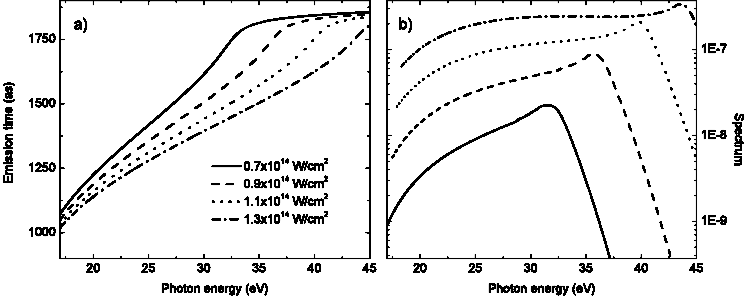
\includegraphics[width=0.8\columnwidth]{Figures/ThreeStep/gdd_argon.pdf}%
\caption{Temps d’émission (gauche) et intensité harmonique (droite) en fonction de l’énergie de photon harmonique et pour différentes intensités de génération. Calcul fait pour l’argon en ne considérant que la trajectoire courte de la GHOE. Tiré de \mycite{DivekiPhD2011}.}
\label{fig:diveki}
\end{figure}

Cette pente linéaire, couramment appelée \textit{atto-chirp}, est donc intrinsèque au mécanisme de génération lui-même \mycite{KazamiasPRA2004}. Elle peut être mesurée expérimentalement, par exemple par la technique RABBIT \mycite{DinuPRL2003,MairesseScience2003}, dont il sera question à la partie \ref{sec:omabbit}. Sa mesure permet également de la compenser, de sorte à comprimer les impulsions attosecondes générées.

\subsection{Phase spatiale des trajectoires quantiques}
\label{sec:phase_spatiale}
Nous avons jusqu'à présent considéré un unique atome émettant un rayonnement harmonique. En réalité, le faisceau de génération a une extension transverse bien plus large qu'un atome, le rayonnement émis est donc la somme cohérente de la contribution de chaque atome unique. Si le faisceau de génération a un profil d'intensité transverse gaussien, son intensité n'est pas uniforme. Nous allons voir que cela se traduit par une phase spatiale non homogène dans l'émission harmonique. On utilise les coordonnées cylindriques $(r,\theta,z)$. En un point $(r,\theta)$ dans le plan transverse, la phase du champ harmonique pour la trajectoire $j$ est donnée par :
\begin{equation}
\phi^j_q = \omega_q t_r - \int_{t_i}^{t_r}\left(\frac{({\bm{p}+\bm{A(t')}})^2}{2}+I_p\right)\rmd t',
\end{equation} 
où $t_i,\;t_r$ et $\bm{p}$ sont les solutions des équations de phase stationnaire. La phase dépend de l'intensité via le potentiel vecteur $\bm{A}(t)$. 

Sur la figure \ref{fig:varju}, tirée de \mycite{VarjuJMO2005}, est tracée $\phi^j_q$ en fonction de l'intensité $I$ pour l'harmonique 19 et pour les deux premières trajectoires quantiques. On observe une dépendance quasiment linéaire, de pente beaucoup plus forte pour la trajectoire longue. Pour les harmoniques loin de l'énergie de coupure, on approxime une dépendance linéaire :
\begin{equation}
\phi^j_q = - \alpha_q^j I,
\label{eq:alphaI}
\end{equation}
où $\alpha_q^j$ est le coefficient de proportionnalité exprimé en $\si{\radian\cm\squared\per\W}$. Cette phase est appelée \textit{phase atomique}. $\alpha_q^{\text{courte}}$ est de l'ordre de $\SI{-1}{\radian\cm\squared\per\W}$ tandis que $\alpha_q^{\text{longue}}\sim\SI{-25}{\radian\cm\squared\per\W}$. Sur le panneau de droite de la figure \ref{fig:varju} est tracé $\partial\phi^j_q/\partial I$ en fonction de l'ordre harmonique. $\alpha_q^{\text{courte}}$ est donc une fonction croissante de l'ordre harmonique, tandis que $\alpha_q^{\text{longue}}$ est décroissante. Dans la coupure, les deux trajectoires se confondent et convergent vers $\approx \SI{-12}{\radian\cm\squared\per\W}$\par
Si on considère maintenant la phase macroscopique du faisceau $\phi^j_q(r,\theta)$ pour une intensité gaussienne, on aura une courbure de phase : la dépendance en intensité du dipôle harmonique modifie la divergence de chaque harmonique. Pour les harmoniques les plus basses, les trajectoires longues auront une divergence bien plus grande que les courtes. Quand l'ordre harmonique augmente, la divergence des trajectoires courtes (resp. longues) augmente (resp. diminue) jusqu'à se confondre à la coupure. Cet effet est bien visible sur les spectres expérimentaux présentés plus loin (figure \ref{Fig:SpectrumGAr}). Il jouera également un rôle central dans la GHOE par un faisceau de Laguerre-Gauss (partie \ref{sec:pmodes}).

\begin{figure}[!ht]
\centering
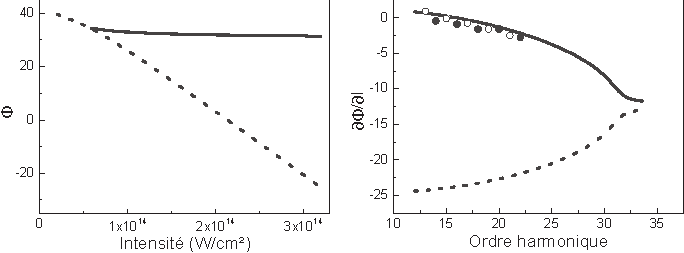
\includegraphics[width=1\columnwidth]{Figures/ThreeStep/alphaI_varju.pdf}%
\caption{Variation de la phase $\phi^j_q$ avec l'intensité (gauche). Le calcul est réalisé pour l'harmonique 19. Variation de $\partial\phi^j_q/\partial I$ avec l'ordre harmonique (droite), à une intensité de $\SI{1.5e15}{\W\per\cm\squared}$. Les lignes continues (resp. pointillées) correspondent aux trajectoires courtes (resp. longues).}
\label{fig:varju}
\end{figure}

\subsection{Accord de phase}
Ces considérations nous amènent à discuter d'un dernier point : l'accord de phase dans la GHOE. Nous avons déjà mentionné que le rayonnement était la somme cohérente de la contribution de chaque atome dans la zone d'interaction. Cette somme doit être réalisé selon la dimension transverse, $(r,\theta)$, et longitudinale, $z$. Si les différentes contributions ne sont pas en phase, des interférences destructives empêcheront l'émission macroscopique de rayonnement XUV. La compréhension de ce phénomène est essentielle pour expliquer les propriétés macroscopiques du rayonnement \mycite{SalieresPRL1995} et pour optimiser le rendement du processus \mycite{KazamiasPRL2003}.

Notons $\bm{k}_q$ le vecteur d'onde de l'harmonique d'ordre $q$ et $\bm{k}_1$ celui du faisceau gaussien de génération. \`A ces deux quantités s'ajoutent des termes de désaccord de phase dus à la phase atomique ainsi qu'à la dispersion électronique et ionique, que l'on note $\Delta \psi_q(r,\theta)$. La condition d'accord de phase pour l'harmonique $q$ s'écrit alors \mycite{BalcouPRA1997} :
\begin{equation}
\bm{k}_q(r,\theta,z) = q\bm{k}_1(r,\theta,z) + \Delta \psi_q(r,\theta,z)
\end{equation}
\mycite{BalcouPRA1997} évaluent le désaccord de phase $|\delta \bm{k}_q| = |\bm{k}_q-q\bm{k}_1 - \Delta \psi_q|$, en négligeant les effets de dispersion sur le laser. La figure \ref{fig:balcou} montre ce désaccord de phase pour les trajectoires courtes et longues. 

\begin{figure}[!ht]
\centering
\includegraphics[width=1\columnwidth]{Figures/ThreeStep/phasematching_balcou.pdf}%
\caption{Désaccord de phase pour les trajectoires longues (gauche) et courtes (droite). Les zones les plus claires indiquent un bon accord de phase. Les pointillés verticaux indiquent les positions des optima de génération d'harmonique. Les flèches représentent la direction d'émission du champ harmonique. Le calcul a été réalisé à une intensité de de \SI{6e14}{\W\per\cm\squared} dans le néon, pour l'harmonique 45. Le paramètre confocal est de 5 mm. Tiré de \mycite{BalcouPRA1997}.}
\label{fig:balcou}
\end{figure}

\'Etudions le cas de la trajectoire longue. On observe une structure particulière, en forme de "moustache de morse". On a deux zones notée B et D où le désaccord de phase est minimisé. La zone notée B est située sur l'axe optique mais est très fine, tandis que la zone D est assez étendue et est située en dehors de l'axe optique. De par le volume disponible, la génération d'harmonique proviendra principalement de la zone D. Les flèches indiquent une émission très divergente, ce qui est dû à l'effet de la phase atomique décrit plus haut. Notons également que la zone D se situe en amont de $z=0$, position du foyer du laser de génération. Pour la trajectoire courte (panneau de droite), le comportement est plus simple : on a un maximum du désaccord de phase vers $z\approx-0.5$ mm, qui diminue ensuite dans toutes les directions. Si on s'éloigne trop du foyer laser, l'intensité devient trop faible pour avoir une génération efficace. \mycite{BalcouPRA1997} montrent que l'optimum se situe à $z=3$ mm, où on a un désaccord faible sur un grand volume. 

En conclusion, nous avons mis en évidence deux familles de trajectoires électroniques, qui donnent lieu à deux composantes dans l'émission harmoniques de propriétés différentes. Finalement, nous avons vu que l'accord de phase permet de favoriser l'une ou l'autre : la trajectoire courte sera accordée lorsque le foyer optique se situe en amont du jet de gaz, tandis que la longue le sera lorsqu'il se situe en aval. Pour une description plus complète de la théorie de la GHOE, on se reportera à \mycite{ScrinziJPB2006} et à \mycite{SmirnovaIvanov2014}. Le modèle SFA présenté ici est la base des calculs numériques présentés plus loin (partie \ref{sec:sfa}), qui prendront en compte tous les effets de propagation et d'accord de phase dans le milieu. Dans la suite de cette partie, nous expliquons comment réaliser une expérience de GHOE dans le cas habituel d'un faisceau de génération gaussien.

\chapter{Aspects expérimentaux de la génération d'harmoniques d'ordre élevé}
\label{Sec:HHG_G}
\section{Système laser}
\label{sec:laser}
Toutes les expériences présentées dans ce chapitre et dans la partie \ref{PA:OAM_HHG} ont été réalisées sur le laser LUCA (Laser Ultra-Court Accordable) du LIDYL au CEA Saclay. Il s'agit d'un laser basé sur la technique "Chirped Pulse Amplification" utilisant le titane saphir comme milieu à gain. Partant d'un oscillateur femtoseconde oscillant autour de 800 nm, le faisceau est étalé temporellement avant d'être amplifié d'abord dans un amplificateur régénératif, puis dans un amplificateur multi-passages. Il est finalement recomprimé dans un compresseur à réseaux \mycite{StricklandOC1985}. La spécificité de ce système est l'insertion récente, juste avant la compression, d'un étage de filtrage modal \mycite{MahieuAPB2015}. Il s'agit d'une fibre creuse de 30 cm de long et $\SI{128}{\micro\metre}$ de diamètre dans laquelle le faisceau est injecté avant d'être collimaté de nouveau. Ceci a pour effet de sélectionner un mode de propagation très proche d'un mode gaussien pur. Finalement on obtient des impulsions dont l'intensité a une enveloppe temporelle gaussienne de largeur à mi-hauteur $\tau = 50$ fs et un profil spatial gaussien de largeur $w_0 = 15$ mm à $\frac{1}{e^2}$. La longueur d'onde utilisée est 792 nm, et l'énergie par impulsion est de 35 mJ pour un taux de répétition de 20 Hz. 

\section{Génération d'harmoniques d'ordre élevé}
Nous commençons par mettre en forme le faisceau laser : son diamètre est ajusté à l'aide d'un iris et son énergie est ajustée grâce à un atténuateur constitué d'une lame demi-onde et d'une paire de polariseur croisés. \`{A} la sortie de cet atténuateur, la polarisation du laser est verticale (S). Le faisceau est ensuite focalisé par une lentille dans un jet de gaz délivré par une vanne pulsée à la fréquence du laser par un système piezo-électrique (Attotech). L'utilisation d'une vanne pulsée permet de n'envoyer du gaz que lorsque le faisceau laser est présent, ce qui limite la pression résiduelle dans les chambres à vide. Ainsi, on peut atteindre une pression assez élevée ($\simeq$10 mbar) dans la région focale sans que l'émission harmonique ne soit réabsorbée par le gaz résiduel. Un autre paramètre important est le diamètre de l'orifice de la vanne (ici, 150 $\si{\micro\metre}$) : en choisissant un diamètre faible, on crée une extension supersonique du gaz ce qui garantit une longueur d'interaction avec le laser courte dans la direction longitudinale. On s'approche ainsi des conditions idéales d'un plan d'atomes, ce qui limite l'importance des effets d'accord de phase dans la GHOE. \par
Le choix du gaz dépend de l'expérience réalisée : on peut par exemple utiliser une molécule dont on étudie la réponse - c'est le principe de la spectroscopie harmonique. Dans notre cas le gaz n'est pas l'objet d'étude et on préférera utiliser un système simple, facile à se procurer, et ayant une grande section efficace. Le gaz le plus courant est l'Argon, qui est peu coûteux et génère de manière très efficace. Son potentiel d'ionisation est de 15.76 eV, ce qui donne une énergie de coupure assez faible et qui empêche de générer des ordres harmoniques très élevés. Dans les cas où on désire générer des ordres élevés et nombreux, on pourra utiliser d'autres gaz rares comme le Néon ($I_p$ = 21.6 eV), bien que la génération soit moins efficace.

Pour notre système, les paramètres nominaux sont :
\begin{itemize}
\item Le diamètre avant focalisation \O{} $\approx$ 10-15 mm,
\item L'énergie par impulsion de l'ordre de E = 1-3 mJ,
\item La lentille de longueur focale f = 1 m. \\
\end{itemize}
Pour connaître la valeur de l'intensité pic au foyer, le profil du faisceau après focalisation peut être calculé numériquement. Le champ avant la lentille est défini dans les coordonnées cylindriques $(R,\theta)$ par :
\begin{equation*}
E(R,\theta) = \sqrt{I_0} \exp{\left(-\frac{R^2}{w_0^2}\right)}\times\delta(\frac{\mbox{\O}}{2}-R),
\end{equation*}
où $w_0$ est la largeur du faisceau collimaté avant l'iris, \O{}  est le diamètre de l'iris, $\delta$ est la fonction de Heaviside, et $I_0 = \frac{2E\sqrt{\frac{4\log{2}}{\pi}}}{\tau\pi w_0^2}$.
La focalisation d'un faisceau par une lentille mince peut être calculée par une transformée de Fourier (voir \mycite{Goodman}, un des ouvrages de référence pour l'optique de Fourier, et \mycite{Tan} pour des exemples d'implémentations numériques). Ces calculs permettent d'étudier l'influence des différents paramètres. Par exemple, on peut faire varier le diamètre de l'iris : la Figure \ref{Fig:IrisScan} montre le profil du faisceau au foyer quand \O{} varie entre 5 et 25 mm. On voit alors que l'intensité pic au foyer part d'une valeur $<10^{13}$ et monte jusqu'à $\SI{10e14}{W/cm²}$. On se trouve donc parfaitement dans le régime d'intensité nécessaire à la génération d'harmonique : l'intensité est suffisante pour enclencher une ionisation tunnel mais reste assez faible pour ne pas ioniser et dépléter tout le milieu.

\begin{figure}[!ht]
\centering
\def\svgwidth{\columnwidth}
\import{Figures/Iris_Scan/}{Fig_IrisScan.pdf_tex}
\caption{\'{E}volution du foyer lorsqu'on varie la taille de l'iris. De gauche à droite : (1) profil transverse de l'intensité au foyer, (2) intensité pic, (3) taille du waist. Les paramètres sont les suivants : E = 1 mJ, $w_0$ = 15 mm, $\tau$ = 50 fs, $\lambda$ = 792 nm, f = 1 m et \O{} variant de 5 à 25 mm par pas de 1 mm. Le calcul est réalisé sur une grille de 1025x1025 points correspondant à une taille réelle de 5*\O{}.}
\label{Fig:IrisScan}
\end{figure}

Les harmoniques d'ordre élevé du laser infrarouge sont ainsi générées par le gaz injecté près du foyer de la lentille. Pour leur détection et caractérisation, nous avons utilisé d'une part un spectromètre électronique à temps de vol, d'autre part un spectromètre de photons. Le premier requiert un rayonnement focalisé alors que le second accepte en entrée un rayonnement divergent. Afin de pouvoir utiliser ces deux diagnostics successivement, avant d'entrer dans le spectromètre, le rayonnement XUV est ré-imagé par un dispositif composé de deux optiques (représentées plus bas sur la figure \ref{Fig:ExpG}) :
\begin{enumerate}
\item Un miroir torique en or de 50 cm de focale. Le miroir travaille à $11.5\degres$ d'incidence rasante ($78.5\degres$ par rapport à la normale au miroir), ce qui permet d'avoir une réflectivité importante et plate sur la gamme spectrale considérée (voir Figure \ref{Fig:TorR}).

\begin{figure}[!ht]
\centering
\def\svgwidth{0.6\columnwidth}
\import{Figures/Reflect_Torique/}{torR.pdf_tex}
\caption{Réflectivité calculée du miroir torique en or à un angle d'incidence de $11.5\degres$. (CXRO, \mycite{Henke1993}).}
\label{Fig:TorR}
\end{figure}
Le miroir torique est utilisé dans une configuration 2f-2f de sorte à garder un rapport\shorthandoff{:} 1:1 \shorthandon{:}entre le foyer de génération et le second foyer. \`{A} la position de ce second foyer nous pouvons placer le spectromètre à temps de vol, qui sert dans le cas d'une mesure RABBIT (voir la partie \ref{sec:omabbit}). Un autre avantage de cette imagerie est d'éloigner la zone de génération, où la pression est élevée, du spectromètre de photons, qui requiert un vide de l'ordre de $10^{-5}$ mbar pour que les détecteurs fonctionnent.\\

\item La deuxième optique est une lame de Si$\mbox{O}_{\mbox{2}}$, qui joue le rôle de filtre de l'infrarouge de génération. La lame de silice est traitée antireflet pour l'infrarouge grâce à un dépôt de multicouches. La dernière de ces couches est en silice, ce qui, combiné à une bonne qualité de surface permet de réfléchir efficacement le rayonnement harmonique. La Figure \ref{Fig:SilR}, tirée de \mycite{MairessePhD}, présente la réflectivité de la lame pour le rayonnement harmonique et infrarouge. La réflectivité dans l'extrême ultra violet (XUV) est donc supérieure à 50\% jusqu'à l'ordre $\approx 37$, tandis que moins de 10\% de l'infrarouge est réfléchi. Le filtrage de l'infrarouge de génération est souvent crucial : il constitue un bruit de mesure non négligeable, sans compter qu'il peut facilement endommager des optiques ou des détecteurs en aval s'il est focalisé.

\begin{figure}[!ht]
\centering
\def\svgwidth{\columnwidth}
\import{Figures/Reflect_Silice/}{silR.pdf_tex}
\caption{Réflectivité de la lame de silice. \`{A} gauche, transmission et réflectivité à 800 nm en fonction de l'angle d'incidence rasante. Les pointillés repèrent notre angle de $11.5\degres$. \`{A} droite, réflectivité XUV mesurée (cercles bleus) et donnée par le CXRO (ligne violette) (\mycite{Henke1993}). Figure adaptée de \mycite{MairessePhD}.}
\label{Fig:SilR}
\end{figure}
\end{enumerate}

Comme nous le verrons plus loin, pour l'étude des faisceaux de Laguerre-Gauss, il sera crucial d'imager le spectre harmonique, c'est-à-dire de séparer les différents ordres harmoniques et de mesurer leurs propriétés spatiales. C'est le rôle du spectromètre de photons. Environ 50 cm en aval du second foyer, les harmoniques sont dispersées par un réseau à pas variable cylindrique Hitachi 001-0437 (voir \mycite{KitaAO1983} pour des détails sur son fonctionnement). Comme pour les réseaux à pas fixe, l'angle de réflexion d'un rayonnement monochromatique de longueur d'onde $\lambda$ est donné par la formule :
\begin{equation*}
m\lambda=\frac{\sin{\alpha}+\sin{\beta}}{\sigma},
\end{equation*}
où $m$ est l'ordre de diffraction considéré (généralement 1), $\sigma$ le nombre de trait par mètre (1200 traits/mm dans notre cas), $\alpha$ et $\beta$ les angles d'incidence et de réflexion, définis par rapport à la normale au réseau (la documentation donne $\alpha = 87$\degres{} pour un fonctionnement optimal).\par
Le réseau de diffraction est cylindrique, le rendant focalisant uniquement dans la dimension horizontale. Un rayonnement gaussien de faible largeur spectrale $\Delta\lambda$ et de largeur spatiale $w(z)$ formera donc dans le plan focal du réseau une fine ligne verticale de largeur proportionnelle à $\Delta\lambda$ et de hauteur $w(z)$. On image ainsi à la fois les dimensions spectrale et spatiale, si on suppose la symétrie cylindrique. Ce spectre est imagé par des galettes de micro-canaux couplées à un écran de phosphore, lui-même observé par une caméra CCD Basler A102f. 

L'intégralité du dispositif expérimental est représenté sur la Figure \ref{Fig:ExpG}.

\vspace{\baselineskip}
\begin{figure}[!ht]
\centering
\def\svgwidth{\columnwidth}
\import{Figures/Setup_G/}{setupG_wbitmap.pdf_tex}
\caption{Dispositif expérimental de génération et détection d'harmoniques d'ordre élevé.}
\label{Fig:ExpG}
\end{figure}

Les figures \ref{Fig:SpectrumGAr} et \ref{Fig:SpectrumGNe} présentent des spectres obtenus avec ce dispositif en utilisant respectivement l'argon et le néon comme gaz de génération. On observe les ordres harmoniques allant de 13 à 29 dans l'argon, et de 13 à 57 dans le néon. Le potentiel d'ionisation du Néon, plus élevé que celui de l'argon, a permis d'utiliser une intensité plus importante sans ioniser complètement le milieu. Conformément à la loi de coupure on obtient dans ce cas un spectre plus étendu. Sur le spectre de l'argon, on observe clairement les deux premières trajectoires quantiques de la GHOE (voir partie \ref{sec:thTraj}) : une contribution sur l'axe correspond à la trajectoire courte et une plus divergente et moins intense correspond à la trajectoire longue. Dans le cas du néon, les conditions d'accord de phase utilisées favorisent la trajectoire courte. On remarque également que la divergence de la trajectoire courte (resp. longue) augmente (rep. diminue) avec l'ordre harmonique, jusqu'à ce que les deux trajectoires se confondent dans la coupure. Notons finalement la présence sur le spectre du néon de pics satellites autour des harmoniques les plus basses : il s'agit des harmoniques plus élevées diffractées au second ordre par le réseau.
\begin{figure}[!ht]
\centering
\def\svgwidth{\columnwidth}
\import{Figures/Spectrum_G/}{Spectrum_G_Ar.pdf_tex}
\caption{Spectre d'harmoniques d'ordre élevé générées dans l'argon à partir d'un mode laser gaussien.}
\label{Fig:SpectrumGAr}
\end{figure}
\begin{figure}[!ht]
\centering
\def\svgwidth{\columnwidth}
\import{Figures/Spectrum_G/}{Spectrum_G_Ne.pdf_tex}
\caption{Spectre d'harmoniques d'ordre élevé générées dans le néon à partir d'un mode laser gaussien.}
\label{Fig:SpectrumGNe}
\end{figure}

\chapter{Le moment angulaire de la lumière}
\label{CH:LightAM}

Dans ce chapitre, nous nous attacherons d'abord à définir le moment angulaire (MA) classiquement, dans le cas d'un objet quelconque puis pour le champ électromagnétique, en utilisant l'optique maxwellienne. Nous étudierons ensuite l'équation d'onde et le moment angulaire de plusieurs de ses solutions, mettant en évidence deux types de MA de nature différente. Pour comprendre la natures de ces MA, nous étudierons le concept de moment angulaire en mécanique quantique, où on trouvera deux composantes du moment angulaire : le moment angulaire de spin (MAS) et le moment angulaire orbital (MAO). Le champ électromagnétique sera traité comme un système quantique, ce qui nous permettra de construire des champs pour lesquels le MAS et le MAO sont connus. En particulier, nous détaillerons la forme et les propriétés de ces champs. Nous terminerons par une discussion de l'échange de moment angulaire lors d'une interaction entre un laser et une molécule. Cette présentation nous fournira les outils utiles à l'analyse des expériences décrites dans le chapitre suivant.
\newpage
\section{Le moment angulaire en physique classique}
\subsection{Mécanique Lagrangienne}
\subsubsection{L'\'{e}quation de Lagrange}
\label{sec:lagrange}
En mécanique classique, l'évolution d'un objet est décrite par les lois de Newton. Pour un objet ponctuel, on a $\bm{F}=m\bm{\ddot{x}}$, où $\bm{F}$ est la somme des forces appliquées à cet objet, $m$ sa masse et $\bm{\ddot{x}}$ son accélération. Dans le cas d'objets plus complexes tels que ceux qui nous intéresserons dans ce chapitre, une description plus adaptée est celle développée par J.-L. Lagrange en 1764. Initialement utilisé pour l'étude de la libration de lune, ce formalisme a très largement dépassé son origine pour devenir une méthode générale de résolution de problèmes dynamiques. Le système y est décrit par un ensemble de \textit{coordonnées généralisées}, qui définissent l'espace des configuration. 

Par exemple, considérons un ensemble de particules soumises à un ensemble de forces conservatives décrites par un potentiel. De manière générale, on peut décrire l'état du système par un ensemble de coordonnées. Si on choisit les coordonnées cartésiennes dans un référentiel inertiel ${x_i}$, $i\in[1,\;N]$, l'équation de Newton s'écrit :
\begin{equation}
\label{eq:newton}
\forall i,\;m\ddot{x}_i = F_i.
\end{equation}
Remarquons que le terme de gauche est la dérivée de la quantité de mouvement $p_i=m\dot{x}_i=\partial T/\partial\dot{x}_i$, où $T$ est l'énergie cinétique. Le terme droite est la dérivée de l'énergie potentielle, $\partial U/\partial x_i$. Dans ces coordonnées, $T$ est indépendant de $x_i$ et $U$ est indépendant de $\dot{x}_i$. On définit alors le \textbf{Lagrangien} $L=T-U$, qui est une fonction des $x_i$ et des $\dot{x}_i$. On réécrit alors \ref{eq:newton} :
\begin{equation}
\label{eq:lag}
\frac{d}{dt}\frac{\partial L}{\partial \dot{x}_i}-\frac{\partial L}{\partial x_i}=0,
\end{equation}
qui est appelée \textbf{équation de Lagrange}. Montrons que cette équation est valable quels que soient les coordonnées généralisée utilisée pour décrire le système. Supposons que l'espace des configurations soit décrit par ${q_j}$, $j\in[1,\;N]$, qui s'écrivent en fonction des coordonnées cartésiennes ${x_i}$ et du temps :
\begin{equation*}
\begin{split}
\forall j, q_j=q_j(x_1,\ldots,x_N,t)\text{ et inversement, }
\end{split}
\begin{split}
\forall i, x_i=x_i(q_1,\ldots,q_N,t).
\end{split}
\end{equation*}
Réécrivons l'équation de Lagrange \ref{eq:lag} en fonction des ${q_j}$. On a : 
\begin{equation}
\label{eq:lag1}
\frac{\partial L}{\partial \dot{x}_i} = \sum_j \frac{\partial L}{\partial q_j} \frac{\partial q_j}{\partial \dot{x}_i}+ \sum_j\frac{\partial L}{\partial \dot{q}_j}\frac{\partial \dot{q}_j}{\partial \dot{x}_i}.
\end{equation}
$q_j$ ne dépend que de $x_i$ et $t$, donc ${\partial q_j}/{\partial \dot{x}_i}=0$ et le premier terme s'annule. De plus,
\begin{equation}
\dot{q}_j = \sum_i \frac{\partial q_j}{\partial x_i}\dot{x}_i+\frac{\partial q_j}{\partial t}\text{,  donc  }
\frac{\partial \dot{q}_j}{\partial \dot{x}_i}=\frac{\partial q_j}{\partial x_i}.
\label{eq:lag3}
\end{equation}
\ref{eq:lag1} donne donc :
\begin{equation}
\label{eq:lag2}
\frac{\partial L}{\partial \dot{x}_i} = \sum_j\frac{\partial L}{\partial \dot{q}_j}\frac{\partial q_j}{\partial x_i}.
\end{equation}
L'équation de Lagrange en coordonnées cartésiennes comprend la dérivée temporelle de cette expression, qui s'écrit :
\begin{align*}
\frac{d}{dt}\frac{\partial L}{\partial \dot{x}_i} &= 
\sum_j\left(\frac{d}{dt}\frac{\partial L}{\partial \dot{q}_j}\right)\frac{\partial q_j}{\partial x_i}+
\sum_j\frac{\partial L}{\partial \dot{q}_j}\left(\frac{d}{dt}\frac{\partial q_j}{\partial x_i}\right) \\
&=\sum_j \left(\frac{d}{dt}\frac{\partial L}{\partial \dot{q}_j}\right)\frac{\partial q_j}{\partial x_i}+\sum_j\frac{\partial L}{\partial \dot{q}_j}\left(\sum_k \frac{\partial^2q_j}{\partial x_i \partial x_k}\dot{x}_k + \frac{\partial^2q_j}{\partial x_i \partial t}\right).
\end{align*}
Par ailleurs, le second terme de l'équation de Lagrange s'écrit :
\begin{align*}
\frac{\partial L}{\partial x_i}&= \sum_j \frac{\partial L}{\partial q_j} \frac{\partial q_j}{\partial x_i}+ \sum_j\frac{\partial L}{\partial \dot{q}_j}\frac{\partial \dot{q}_j}{\partial x_i} \\
&=\sum_j \frac{\partial L}{\partial q_j} \frac{\partial q_j}{\partial x_i}+ \sum_j\frac{\partial L}{\partial \dot{q}_j}\left(\sum_k \frac{\partial^2q_j}{\partial x_i \partial x_k}\dot{x}_k + \frac{\partial^2q_j}{\partial x_i \partial t}\right),
\end{align*}
où on a utilisé \ref{eq:lag3}. On connaît maintenant tous les termes de l'équation de Lagrange en fonction des ${q_j}$, et en les soustrayant un terme s'annule, ce qui donne :
\begin{equation*}
\sum_j\left(\frac{d}{dt}\frac{\partial L}{\partial \dot{q}_j}-\frac{\partial L}{\partial q_j}\right)\frac{\partial q_j}{\partial x_i}=0.
\end{equation*}
$\frac{\partial q_j}{\partial x_i}$ est non singulière puisque son inverse est $\frac{\partial x_i}{\partial q_j}$, on obtient donc l'équation de Lagrange en coordonnées généralisées : 
\begin{equation}
\label{eq:lagq}
\frac{d}{dt}\frac{\partial L}{\partial \dot{q}_i}-\frac{\partial L}{\partial q_i}=0.
\end{equation}
Nous avons donc démontré que l'équation de Lagrange est invariante par changement des coordonnées utilisées pour décrire le système, ce qui en fait une formulation très pratique. 

\subsubsection{Symétries du Lagrangien et loi de conservation}
L'équation de Lagrange permet d'obtenir des résultats généraux assez directement, tels que des lois de conservation. Une coordonnée $q_k$ est dite \textit{ignorable} ou \textit{cyclique} si le Lagrangien $L$ ne dépend pas de $q_k$. L'équation de Lagrange donne alors :
\begin{equation*}
\frac{d}{dt}\frac{\partial L}{\partial \dot{q}_k} = \frac{\partial L}{\partial q_k} = 0.
\end{equation*}
On définit naturellement la grandeur 
\begin{equation*}
P_k\equiv\frac{\partial L}{\partial \dot{q}_k},
\end{equation*}
appelé \textit{moment généralisé conjugué} de $q_k$, et qui est une constante du mouvement. Nous allons utiliser ce point pour établir trois lois de conservation : l'énergie, la quantité de mouvement et le moment angulaire.

\paragraph*{\'{E}nergie et translation dans le temps}
La dérivée temporelle du Lagrangien s'écrit : 
\begin{align*}
\frac{dL}{dt}&=\sum_i\frac{\partial L}{\partial q_i}\frac{\partial q_i}{\partial t}+\sum_i\frac{\partial L}{\partial \dot{q}_i}\frac{\partial \dot{q}_i}{\partial t}+\frac{\partial L}{\partial t}\\
&= \sum_i\left(\frac{d}{dt}\frac{\partial L}{\partial \dot{q}_i}\right)\frac{\partial q_i}{\partial t}+\sum_i\frac{\partial L}{\partial \dot{q}_i}\frac{\partial \dot{q}_i}{\partial t}+\frac{\partial L}{\partial t}\\
&= \sum_i\frac{d}{dt}\left(\frac{\partial L}{\partial \dot{q}_i}\dot{q}_i\right)+\frac{\partial L}{\partial t}.
\end{align*}
Soit :
\begin{equation*}
\frac{d}{dt}\left(\sum_i\frac{\partial L}{\partial \dot{q}_i}\dot{q}_i-L\right)+\frac{\partial L}{\partial t}=0.
\end{equation*}
On définit alors la \textit{fonction énergie}\footnote{La fonction énergie semble avoir la même définition que l'Hamiltonien $H$ du système. Ils sont en effet égaux en valeur mais de nature différente : $h$ est une fonction des $N$ variables ${q_i}$, de leurs dérivées et éventuellement le temps, tandis que $H$ est une fonction de $2N$ variables ${q_i,p_i}$ et éventuellement du temps. Cette distinction est centrale pour la définition de la physique Hamiltonienne.} ou \textit{invariant de Jacobi} :
\begin{equation*}
h(q,\dot{q},t) = \sum_i\frac{\partial L}{\partial \dot{q}_i}\dot{q}_i-L,
\end{equation*}
on a donc 
\begin{equation*}
\frac{dh}{dt} = -\frac{\partial L}{\partial t}
\end{equation*}
On voit que si le Lagrangien ne dépend pas explicitement du temps, i.e. est invariant par translation temporelle, alors $h$ est conservé. Dans de nombreux cas, $h$ peut se réduire à l'énergie mécanique du système (voir p. 62 de \mycite{Goldstein2001}). Le résultat obtenu est alors la \textit{conservation de l'énergie mécanique}. 


\paragraph*{Quantité de mouvement et translation dans l'espace}
Considérons maintenant un système invariant par translation dans l'espace. C'est le cas d'une particule libre, ou encore de $N$ particules reliées par des interactions ne dépendant que de leur coordonnées relatives $\left|\bm{r}_i-\bm{r}_j\right|$. 
On note $\bm{r}_i(t)$ la trajectoire des particules et on considère une translation infinitésimale du système de coordonnées : $\bm{r}_i\rightarrow \bm{r}_i+\epsilon$. Le changement du Lagrangien vaut :
\begin{align*}
\delta L =\sum_i \epsilon\cdot\frac{\partial L}{\partial \bm{r}_i}= \epsilon\cdot\frac{d}{dt}\sum_i \frac{\partial L}{\partial {\dot{\bm{r}}}_i}
\end{align*}
Si le système est invariant par rapport à la translation, alors $\delta L=0$ et la quantité de mouvement totale
\begin{equation*}
\bm{P}\equiv\sum_i\frac{\partial L}{\partial \dot{\bm{r}}_i}
\end{equation*}
est conservée. Si l'invariance n'est vraie que dans une direction, alors seulement la composante de $\bm{P}$ dans cette direction sera conservée.


\paragraph*{Moment angulaire et rotation}
Enfin, considérons un système invariant par rotation autour d'un axe $\bm{u}$. Prenons une rotation infinitésimale d'angle $\delta\theta$ et notons $\delta\bm{\theta}=\bm{u}\delta\theta$. Si on choisit l'origine du repère sur l'axe de rotation, le changement pour chaque vecteur de coordonnées est $\delta\bm{r}_i(t) = \delta\bm{\theta}\times\bm{r}_i(t)$. De même, $\delta\bm{\dot{r}}_i(t) = \delta\bm{\theta}\times\bm{\dot{r}}_i(t)$. Le changement du Lagrangien est :
\begin{align*}
\delta L &=\sum_i \left(\delta\bm{\theta}\times\bm{r}_i(t)\right)\cdot\frac{\partial L}{\partial \bm{r}_i}+\sum_i \left(\delta\bm{\theta}\times\bm{\dot{r}}_i(t)\right)\cdot\frac{\partial L}{\partial \bm{\dot{r}}_i}\\
&=\delta\bm{\theta}\cdot\sum_i\left(\bm{r}_i(t)\times\frac{d}{dt}\frac{\partial L}{\partial {\dot{\bm{r}}}_i}
+\bm{\dot{r}}_i(t)\times\frac{\partial L}{\partial \bm{\dot{r}}_i}\right)\\
&=\delta\bm{\theta}\cdot\sum_i\frac{d}{dt}\left(\sum_i \bm{r}_i(t)\times\frac{\partial L}{\partial \bm{\dot{r}}_i}\right)
\end{align*}
où on a permuté circulairement les produits mixtes et utilisé l'équation de Lagrange. Si le Lagrangien est invariant par rotation, alors $\delta L = 0$ et on note $\bm{J}$ la quantité conservée suivante :
\begin{equation}
\bm{J}\equiv\sum_i \bm{r}_i(t)\times\frac{\partial L}{\partial \bm{\dot{r}}_i}=\sum_i \bm{r}_i\times\bm{p}_i.
\label{eq:defJ}
\end{equation}
$J$ est le \textit{moment angulaire} du système. Il est clair que sa valeur dépend du choix du centre du système de coordonnées. Si on applique $\bm{r}_i\rightarrow \bm{r}_i+\bm{a}$, alors $\bm{J}_i\rightarrow \bm{J}+\bm{a}\times\bm{P}$. Notons que dans le référentiel du centre de masse (c.d.m.), $\bm{P}=0$. $\bm{J}$ est alors indépendant du choix de l'origine des coordonnées. Pour des raisons qui paraîtront claires plus tard, notons $\bm{S}$ la valeur de $\bm{J}$ dans le référentiel du c.d.m. Dans un référentiel où le c.d.m se déplace à une vitesse uniforme $\bm{V}$, 
\begin{align*}
\bm{J}&=\sum_i \left(\bm{r}_i+\bm{V}t\right)\times\left(\bm{p}_i+m_i\bm{V}\right)\\
&= \sum_i\bm{r}_i\times\bm{p}_i+\bm{V}t\times\bm{P}+\sum_i m_i\bm{r}_i\times\bm{V} \\
&= \bm{S} + M \bm{R}_{cdm}\times\bm{V} = \bm{S} + \bm{R}_{cdm}\times\bm{P}.
\end{align*}
où $M=\sum_i m_i$ est la masse totale du système et $\bm{R}_{cdm}$ la position du centre de masse. On décompose donc le moment angulaire total en deux parties : $\bm{S}$, qui est indépendante du choix du repère, et $\bm{R}_{cdm}\times\bm{P}$.

\subsection{Les propriétés mécaniques de la lumière}
Comme nous l'avons fait pour la matière, nous établissons ici les expressions de l'énergie, de la quantité de mouvement et du moment angulaire associé à un rayonnement électromagnétique.

\subsubsection{L'énergie du champ électromagnétique} 
Définir l'énergie du champ électromagnétique a donné lieu à de vifs débats à la fin du XIXème siècle, liés aux discussions sur la propagation d'une onde dans le vide. Dans une série de travaux pionniers, John H. Poynting a largement clarifié les dicussions au sujet de l'énergie des ondes électromagnétiques, la pression de radiation, et même le moment angulaire de la lumière. Poynting faisait partie d'un groupe de physiciens mené par Heaviside, Fitzgerald, Lodge et Hertz qui travaillèrent à développer la théorie de Maxwell après sa mort en 1873. Nous reprenons ici la démarche de son article de 1884 \mycite{Poynting1884}, qui amène à une expression de la densité d'énergie et du flux d'énergie d'un champ électromagnétique.

Considérons une distribution de charges et de courants contenus dans un volume $V$. En un court temps $\rmd t$, une charge bougera de $\bm{v}\rmd t$. En utilisant l'expression de la force de Lorentz, le travail effectué sur la charge sera
\begin{equation*}
\rmd W = \bm{F}\cdot\bm{\rmd l} = q(\bm{E}+\bm{v}\times\bm{B})\cdot\bm{v}\rmd t = q\bm{E}\cdot \bm{v} \rmd t,
\end{equation*}
où l'on retrouve que la force magnétique ne fournit pas de travail. Notons ensuite $\rho$ la densité de charge dans le volume ($q = \rho \rmd V$) et $\bm{J} =\rho \bm{v}$ la densité de courant. En intégrant sur le volume V, on obtient
\begin{equation*}
\frac{\rmd W}{\rmd t} = \int_V \bm{E} \cdot \bm{J} \rmd V.
\end{equation*}
$\rmd W/\rmd t$ est le taux auquel le travail est fourni, c'est-à-dire la puissance délivrée au système. $\bm{E} \cdot \bm{J}$ est donc la puissance délivrée par unité de volume, que l'on peut exprimer en utilisant l'équation de Maxwell-Ampère :
\begin{align*}
\bm{E} \cdot \bm{J} &= \frac{1}{\mu_0}\bm{E} \cdot (\bm{\nabla} \times \bm{B})-\epsilon_0\bm{E}\cdot\frac{\partial\bm{E}}{\partial t}\\
&= \frac{1}{\mu_0}\bigl[\bm{B} \cdot (\bm{\nabla} \times \bm{E})-\bm{\nabla} \cdot (\bm{E} \times \bm{B})\bigr]-\epsilon_0\bm{E}\cdot\frac{\partial\bm{E}}{\partial t}\\
&= \frac{1}{\mu_0}\bigl[-\bm{B} \cdot \frac{\partial\bm{B}}{\partial t}-\bm{\nabla} \cdot (\bm{E} \times \bm{B})\bigr]-\epsilon_0\bm{E}\cdot\frac{\partial\bm{E}}{\partial t}
\end{align*}
On note que $\bm{B} \cdot \frac{\partial\bm{B}}{\partial t} = \frac{1}{2}\frac{\partial\bm{B^2}}{\partial t}$ et $\bm{E} \cdot \frac{\partial\bm{E}}{\partial t} = \frac{1}{2}\frac{\partial\bm{E^2}}{\partial t}$ et on obtient
\begin{equation*}
\bm{E} \cdot \bm{J} = -\frac{1}{2}\frac{\partial}{\partial t}\biggl(\epsilon_0\bm{E^2}+\frac{1}{\mu_0}\bm{B^2}\biggl)-\frac{1}{\mu_0}\bm{\nabla} \cdot (\bm{E} \times \bm{B})
\end{equation*}
En intégrant cette équation sur le volume $V$ et en utilisant le théorème d'Ostrogradski sur le dernier terme, elle se réécrit
\begin{equation}
\frac{\partial}{\partial t}\int_V\frac{1}{2}\biggl(\epsilon_0\bm{E^2}+\frac{1}{\mu_0}\bm{B^2}\biggl)\rmd V+\frac{1}{\mu_0} \oint_S(\bm{E} \times \bm{B})\cdot\bm{\rmd S}=-\frac{\rmd W}{\rmd t},
\label{eq:continuityE}
\end{equation}
On identifie deux quantités : 
\begin{equation}
U=\frac{1}{2}\biggl(\epsilon_0\bm{E^2}+\frac{1}{\mu_0}\bm{B^2}\biggr) \mbox{   et   } \bm{\Pi} = \frac{1}{\mu_0}\bm{E}\times\bm{B}
\label{Def.Poynting}
\end{equation}
$U$ est la \textbf{densité d'énergie} (énergie par unité de volume) et $\bm{\Pi}$ est la \textbf{densité de flux d'énergie} (énergie par unité de surface par unité de temps). L'équation \ref{eq:continuityE} est donc une équation de conservation de l'énergie qui se comprend ainsi :

Le taux de variation de l'énergie électromagnétique dans V + L'énergie qui sort du volume en traversant la surface S = L'opposé du travail total effectué par le champ sur les sources dans V.

$\bm{\Pi}$ est connu sous le nom de \textbf{vecteur de Poynting}. De manière intéressante, si on considère une onde plane se propageant selon un vecteur d'onde $\bm{k}$, on voit que $\bm{\Pi}$ est parallèle à $\bm{k}$. Ce n'est pas le cas de manière générale : $\bm{k}$ pointe dans la direction de la vitesse de phase alors que $\bm{\Pi}$ pointe dans celle de la vitesse de groupe. De nombreux exemples montrent que ces quantités sont distinctes, tel que la biréfringence ou le phare attoseconde (\mycite{VincentiPRL2012}). 

\subsubsection{La quantité de mouvement de la lumière}
Nous avons démontré la conservation de l'énergie du système combiné du champ et des particules. De la même façon, la quantité de mouvement de ce système doit être conservée. On note $\bm{P}_{part}$ la somme des quantités de mouvement des particules dans le volume V. La seconde loi de Newton donne :
\begin{equation*}
\frac{d\bm{P}_{part}}{dt}=\int_V \rho \bm{E} + \bm{J}\times\bm{B}\;\rmd V.
\end{equation*} 
On utilise l'équation de Maxwell-Gauss et de Maxwell-Ampère pour écrire :
\begin{align*}
\rho \bm{E} + \bm{J}\times\bm{B} &= \frac{1}{\mu_0} \bm{E}\cdot(\bm{\nabla}\cdot\bm{E})+\epsilon_0 \bm{B}\times\frac{\partial \bm{E}}{\partial t}-\frac{1}{\mu_0}\bm{B}\times(\bm{\nabla}\times\bm{B})\\
&= \frac{1}{\mu_0} \bm{E}\cdot(\bm{\nabla}\cdot\bm{E})+\epsilon_0 
\left(-\frac{\partial}{\partial t}(\bm{E}\times\bm{B})+\bm{E}\times\frac{\partial \bm{B}}{\partial t}\right)
-\frac{1}{\mu_0}\bm{B}\times(\bm{\nabla}\times\bm{B})\\
&= \frac{1}{\mu_0} \bm{E}\cdot(\bm{\nabla}\cdot\bm{E})+\epsilon_0\left(-\frac{\partial}{\partial t}(\bm{E}\times\bm{B})-\bm{E}\times(\bm{\nabla}\times\bm{E})\right)
-\frac{1}{\mu_0}\bm{B}\times(\bm{\nabla}\times\bm{B}).
\end{align*} 
Finalement,
\begin{equation*}
\frac{d\bm{P}_{part}}{dt}+\epsilon_0\frac{d}{dt}\int_V (\bm{E}\times\bm{B})\; \rmd V=\int_V \left[\frac{1}{\mu_0} \bm{E}\cdot(\bm{\nabla}\cdot\bm{E})-\epsilon_0\bm{E}\times(\bm{\nabla}\times\bm{E})
-\frac{1}{\mu_0}\bm{B}\times(\bm{\nabla}\times\bm{B})\right]\rmd V.
\end{equation*} 

Comme démontré dans la section 6.9 de \mycite{Jackson1999}, le terme de droite est le flux du quantité de mouvement vers l'extérieur du volume V à travers la surface S. On identifie donc finalement la quantité de mouvement totale du champ électromagnétique :
\begin{align}
\bm{P}_{champ} &= \epsilon_0\frac{d}{dt}\int_V (\bm{E}\times\bm{B})\; \rmd V \nonumber\\
&= \frac{\bm{\Pi}}{c^2} \mbox{, où $\bm{\Pi}$ est donné par \ref{Def.Poynting}.}
\label{eq:defP}
\end{align}

C'est l'essence de la démarche utilisée par Henri Poincaré en 1900 \mycite{poincare1900}, où il discute de la \textit{``quantité de mouvement de [...] notre fluide fictif''}. Dans ce même article, Poincaré parle de la force exercée par la lumière sur la matière, notion déjà présente chez Maxwell et même chez Kepler appelée \textit{pression électromagnétique}. On l'appelle aujourd'hui plus couramment \textit{pression de radiation}. Poynting développa considérablement ce concept par la suite \mycite{poynting1903}, et nota que malgré sa faible valeur comparée à la force de gravitation, elle pourrait avoir d'importantes conséquences en astronomie. \`{A} raison : par exemple, si la pression de radiation n'avait pas été prise en compte lors du programme Viking, les deux sondes envoyées sur Mars auraient raté l'orbite de la planète d'environ 15000 kilomètres \mycite{Hecht2001}.

\subsubsection{Le moment angulaire de la lumière}
Poynting, en plus de ces contributions majeures, a été le premier à envisager l'existence du moment \textit{angulaire} de la lumière. Il fit l'analogie entre une onde électromagnétique polarisée circulairement et une onde élastique de torsion, suggérant que la lumière possède un moment angulaire et peut fournir un couple à la matière \mycite{PoyntingPRSL1909}. Il propose à la fin de son article un dispositif expérimental constitué d'une série de lames quart d'ondes, permettant de démultiplier cet effet jusqu'à le rendre mesurable. Il conclut toutefois avec pessimisme que \textit{``even with such multiplications, my present experience of light forces does not give me much hope that the effect could be detected, if it has the value suggested by the mechanical model''}.

Il aurait donc probablement été heureux d'apprendre qu'en 1936, R. A. Beth observa cet effet avec un schéma légèrement modifié \mycite{BethPR1936}, confirmant ainsi l'existence du moment angulaire de la lumière. \mycite{DelannoyAPL2005} réalisèrent une expérience similaire en utilisant de la soie d'araignée.\par
L'expression de la densité de moment angulaire du champ est directement obtenue en utilisant la définition \ref{eq:defJ} et l'expression \ref{eq:defP}:
\begin{equation}
\bm{J}(\bm{r})=\bm{r}\times\bm{\bm{P}_{champ}}=\frac{\bm{r}\times\bm{\Pi}}{c^2} = \epsilon_0\bm{r}\times(\bm{E}\times\bm{B})
\label{Eq.DefJEM}
\end{equation}

C'est l'expression classique du moment angulaire du champ électromagnétique, la quantité qui nous intéressera pendant la majorité de cette thèse. Nous allons maintenant étudier le moment angulaire de différentes solutions de l'équation d'onde.

\section{Solutions de l'équation d'onde}
\subsection{Ondes planes et polarisation}
\subsubsection{L'équation d'Helmholtz}
Par simplicité, nous ne considérerons pas la présence de densités de charges ou de courant. Dans ce cas, les équations de Maxwell donnent les équations d'onde :
\begin{align*}
&\nabla^2\bm{E}-\frac{1}{c^2}\frac{\partial^2}{\partial t^2}\bm{E}=0,
&\nabla^2\bm{B}-\frac{1}{c^2}\frac{\partial^2}{\partial t^2}\bm{B}=0.
\end{align*}
On considère maintenant des faisceaux monochromatiques de fréquence angulaire $\omega$. On introduit la notation complexe :
\begin{equation*}
\begin{split}
\bm{E}=\text{Re}[\bm{\mathcal{E}}\exp{(-\rmi\omega t)}]
\end{split}
\quad\text{et}\quad
\begin{split}
\bm{B}=\text{Re}[\bm{\mathcal{B}}\exp{(-\rmi\omega t)}],
\end{split}
\end{equation*}
qui permet d'obtenir l'équation d'Helmhotz :
\begin{align}
&\nabla^2\bm{\mathcal{E}}+k^2\bm{\mathcal{E}}=0,\nonumber\\
&\nabla^2\bm{\mathcal{B}}+k^2\bm{\mathcal{B}}=0,
\label{eq:helmhotz}
\end{align}
où $k=\omega/c$ est le nombre d'onde, norme du vecteur d'onde $\bm{k}$. On considère alors l'ansatz $\bm{\mathcal{E}}=\bm{\mathcal{E_0}}\rme^{\pm\rmi\bm{k}\cdot\bm{r}} = \bm{\mathcal{E_0}}\rme^{\pm\rmi(k_x x + k_y y + k_z z)}$. En l'insérant dans \ref{eq:helmhotz}, on obtient 
\begin{equation*}
k_x^2+k_y^2+k_z^2=\frac{\omega^2}{\rmc^2}
\end{equation*}
On suppose $k_x$, $k_y$, $k_z$ réels et on obtient 
\begin{equation*}
\bm{E}=\text{Re}[\mathcal{E_0}\exp{(\pm\rmi\bm{k}\cdot\bm{r}-\rmi\omega t)}],
\end{equation*}
qui sont appelées les ondes planes. Les solutions avec un signe $+$ (resp. $-$) se propagent dans la direction de (resp. inversement à) $\bm{k}$. Pour que ces solutions vérifient les équations de Maxwell, il reste à vérifier qu'elles sont de divergence nulle : $\bm{\nabla}\cdot\bm{E} = 0$. Par conséquent, $\bm{k}\cdot\bm{\mathcal{E_0}}= 0$ : le champ électrique est nécessairement perpendiculaire à $\bm{k}$, on parle d'onde transverse électrique. La direction du champ $\bm{B}$ est donnée par l'équation de Maxwell-Faraday : en notation complexe, $\bm{\nabla}\times\bm{\mathcal{E}}=-\rmi\omega\bm{\mathcal{B}}$. Ainsi, $\bm{B}$ est perpendiculaire à $\bm{E}$ et $\bm{k}$.

\subsubsection{La polarisation des ondes planes}
On choisit un repère cartésien tel que $\bm{k}=\bm{e_z}$. Un champ électrique transverse s'écrit :
\begin{equation*}
\bm{E}=\begin{pmatrix}
E_{0x}\cos{(\omega t-kz)}\\
E_{0y}\cos{(\omega t-kz-\phi)}\\
0
\end{pmatrix}
\end{equation*}
Le champ électrique décrit donc une ellipse dans le plan transverse. S'il la parcourt dans le sens trigonométrique autour de $\bm{k}$, on dit que la polarisation est elliptique gauche (PEG). Inversement, dans le sens des aiguille d'une montre la polarisation est elliptique droite (PED). On peut se placer dans le repère des axes de l'ellipse de sorte à ce que le champ s'écrive :
\begin{equation*}
\bm{E}=\begin{pmatrix}
E_{0x}\cos{(\omega t-kz)}\\
\pm E_{0y}\sin{(\omega t-kz)}\\
0
\end{pmatrix}
\end{equation*}
Le signe $+$ représente une PEG et $-$ une PED. Dans le cas particulier où $E_{0x}=E_{0y}$, l'ellipse devient un cercle et on dit que la polarisation est circulaire gauche (PCG) ou droite (PCD). Enfin, notons que la phase $\phi$ peut être nulle. Dans ce cas, la polarisation est rectiligne. Cette polarisation peut être construite en effectuant la somme d'une PEG et d'une PED. Inversement, une onde polarisée elliptiquement peut être vue comme la superposition de deux polarisations rectilignes.

\subsubsection{Moment angulaire d'une onde plane circulaire}
Intéressons nous maintenant au moment angulaire porté par ces ondes planes. L'équation \ref{eq:defJ} donne son moment angulaire selon l'axe de propagation: 
\begin{align*}
\bm{J_z}&=(\bm{r}\times\bm{\Pi})\cdot\bm{e_z}\\
&=\frac{1}{\mu_0}(\bm{r}\times[\bm{E}\times\bm{B}])\cdot\bm{e_z}
\end{align*}
Il est clair que pour une onde plane $\bm{J_z}$ s'annule. Ceci contredit ce qui est observé dans l'expérience de Beth \mycite{BethPR1936} déjà mentionnée. En fait, ce cas est singulier : $\Pi_x$ et $\Pi_y $ sont nuls alors que l'extension transverse de l'onde est infinie. On est donc confrontés à une indétermination du type $0\times \infty$. 
Ce problème peut être résolu en restreignant le problème à un volume $V$ où l'on prend en compte rigoureusement les effets de bords, puis en faisant tendre les dimensions du volume vers l'infini : voir \mycite{StewartEJP2005}. Une autre approche intéressante est celle de \mycite{MansuripurOE2005}, qui considère 4 ondes planes se propageant avec un angle $\theta$ par rapport à $z$ dans chacun des quadrants de $(x,y)$. Chacune de ces ondes ayant un vecteur d'onde formant un angle avec $z$, $\bm{J_z}$ est non nul. Quand on somme le moment angulaire de ces 4 ondes, si $\theta$ est assez petit on obtient une quantité ne dépendant pas de $\theta$. Il reste ensuite à faire tendre $\theta$ vers 0 pour retrouver l'onde plane comme cas limite, avec un moment angulaire non nul.

Remarquons pour terminer que dans l'expérience de Beth, la lumière transmet du moment angulaire à un objet qui se met à tourner \textit{sur lui-même}, et pas par rapport au centre du faisceau. Ceci est cohérent avec la structure d'une onde plane : dans le plan transverse, son profil ne dépend pas du tout des coordonnées $(x,y)$. C'est bien sa polarisation, c'est-à-dire sa structure vectorielle intrinsèque, qui lui donne du moment angulaire. 

\subsection{L'approximation paraxiale}


\subsection{Les modes de Hermite-Gauss et de Laguerre-Gauss}


\section{Le moment angulaire en mécanique quantique}
Dans cette partie nous discuterons de la définition du moment angulaire en mécanique quantique. Comme nous le verrons, cette approche est complémentaire de la précédente pour comprendre certaines des propriétés de la lumière portant du moment angulaire. 

\subsection{Symétries et lois de conservation}

Dans la partie précédente, nous avons utilisé les lois de la mécanique classique pour définir la notion de moment angulaire. Nous avons vu que comme la masse ou l'énergie, $J$ était une quantité conservée. En mécanique classique, une loi de conservation est presque toujours le point de départ d'un raisonnement. En mécanique quantique au contraire, il est remarquable que les lois de conservation soient profondément reliées et découlent directement des propriétés de symétrie des systèmes. 

\subsubsection{Définition de la symétrie d'un système}
Nous commençons donc par étudier la question de la symétrie d'un système. Notons $\ket{\psi_1}$ l'état de départ du système et $\ket{\psi_2}$ l'état après un temps $t$. On peut noter $\hat{U}$ l'opérateur définit par :
\begin{equation*}
\ket{\psi_2}=\hat{U}(t,0)\ket{\psi_1},
\end{equation*}
c'est à dire l'opération de faire évoluer le système entre 0 et $t$.

Imaginons maintenant que l'on effectue un certain nombre d'opérations sur le système. Notons $\hat{Q}$ l'ensemble de ces opérations et imaginons que cet opérateur laisse \textit{la physique du système inchangée}. On peut par exemple penser à $H_2$, laissé inchangé par l'opérateur de réflexion par rapport à un plan, ou bien à un système à symétrie sphérique, où une rotation d'angle fini ne change pas la physique. Dans un système à deux électrons, on peut aussi penser à l'opération d'interchanger les deux électrons. \\
Une façon d'écrire cette propriété de ``garder la physique inchangée'' est la suivante : si j'applique $\hat{Q}$ au système, alors $\ket{\psi_1}$ est transformé en $\ket{\psi'_1}=\hat{Q}\ket{\psi_1}$, et $\ket{\psi'_2}=\hat{Q}\ket{\psi_2}$. Mais comme la physique est inchangée par $\hat{Q}$, si on attend un temps $t$ on obtient le même résultat qu'avant d'appliquer $\hat{Q}$, c'est-à-dire :
\begin{align*}
\ket{\psi'_2}&=\hat{U}\ket{\psi'_1}, \mbox{ qu'on peut réécrire}\\
\hat{Q}\ket{\psi_2}&=\hat{U}\hat{Q}\ket{\psi_1}, \mbox{ ou encore}\\
\hat{Q}\hat{U}\ket{\psi_1}&=\hat{U}\hat{Q}\ket{\psi_1}.
\end{align*}
On obtient le résultat que $\hat{U}$ et $\hat{Q}$ commutent. On peut montrer que pour un temps infinitésimal $dt$, on a $\hat{U}(t+dt,t) = 1-i\hat{H}dt/\hbar$, où $\hat{H}$ est l'hamiltonien du système. Cela permet d'écrire :
\begin{equation*}
[\hat{H},\hat{Q}]=0,
\end{equation*}
qui est la \textit{définition} de la symétrie d'un système physique d'hamitonien $\hat{H}$ par rapport à l'opérateur $\hat{Q}$.

\subsubsection{Relation entre symétrie et loi de conservation}
Supposons maintenant qu'une fois l'opérateur $\hat{Q}$ appliqué à notre état, on obtienne un état qui soit \textit{physiquement le même}. C'est-à-dire que $\hat{Q}\ket{\psi_1}$ est égal à $\ket{\psi_1}$ à un facteur de phase près qu'on note $e^{i\delta}$. Après un temps $t$, on obtient $\ket{\psi_2}$ à qui on peut appliquer $\hat{Q}$ :
\begin{align*}
\hat{Q}\ket{\psi_2}&=\hat{Q}\hat{U}(t,0)\ket{\psi_1}=\hat{U}(t,0)\hat{Q}\ket{\psi_1} \mbox{ en utilisant la symétrie du système,}\\
		&=\hat{U}(t,0)e^{i\delta}\ket{\psi_1}=e^{i\delta}\ket{\psi_2}.
\end{align*}

On vient de vérifier qui si la propriété de symétrie est vraie initialement, elle est vraie à n'importe quel autre instant, ce qui ressemble fortement à \textit{une loi de conservation}. C'est en fait exactement le cas : si le système est initialement dans un état à caractère symétrique \textbf{et} que l'hamiltonien du système est symétrique par rapport à cette opération, \textbf{alors} l'état du système aura ce même caractère symétrique à tout instant. C'est de cette relation que découlent les lois de conservation en mécanique quantique, particulièrement utiles puisqu'il n'est pas nécessaire de connaître tout le détail de l'évolution du système au cours du temps. Nous en détaillons quelques unes ici.

\subsubsection{La parité et l'opérateur inversion}
Commençons par appliquer notre résultat au cas de l'opérateur inversion $\hat{P}$, définit par l'opérateur qui change $(x,y,z)$ en $(-x,-y,-z)$. Supposons que l'on ait un état symétrique par rapport à $\hat{P}$ : 
\begin{equation*}
\hat{P}\ket{\psi_1} = e^{i\delta}\ket{\psi_1}.
\end{equation*}
Si on applique deux fois l'opérateur, on obtient bien sûr l'état de départ
\begin{equation*}
\ket{\psi_1} = \hat{P}\cdot\hat{P}\ket{\psi_1} = (e^{i\delta})^2\ket{\psi_1}.
\end{equation*}
On en déduit que $(e^{i\delta})^2=1$, c'est à dire $e^{i\delta}=\pm1$. On voit donc que seulement deux cas sont possibles :
\begin{equation*}
\hat{P}\ket{\psi_1} = \ket{\psi_1} \mbox{ ou } \hat{P}\ket{\psi_1} = -\ket{\psi_1}.
\end{equation*}

Si $\hat{P}\ket{\psi_1}= \ket{\psi_1}$, on dit que $\ket{\psi_1}$ est de parité \textit{paire}, et si $\hat{P}\ket{\psi_1}= -\ket{\psi_1}$, on dit que $\ket{\psi_1}$ est de parité \textit{impaire}. $\hat{P}$ est également appelé opérateur parité. Notons que la grande majorité des lois physiques sont symétriques par rapport à $\hat{P}$. En fait, seule l'interaction faible ne respecte pas cette propriété. Pour tout ce qui va nous intéresser par la suite, on considérera donc toujours que l'hamiltonien de notre système est symétrique par rapport à $\hat{P}$. On en conclut que si le système a une parité définie à un instant, alors il gardera la même parité. C'est ce qu'on appelle \textit{la conservation de la parité}, très importante dans les interactions lumière-matière.

\subsubsection{Le moment angulaire et l'opérateur rotation}
Nous pouvons appliquer la même démarche cette fois en utilisant l'opérateur rotation $\hat{R}_z(\theta)$, défini comme la rotation du système d'un angle $\theta$ autour de l'axe $z$. Dans un problème à symétrie cylindrique, un tel opérateur laisse le système inchangé, à un terme de phase près :
\begin{equation*}
\hat{R}_z(\theta)\ket{\psi_1}=e^{i\delta}\ket{\psi_1}.
\end{equation*}
On peut montrer ($\text{B}_{\text{VI}}$ de \mycite{cohen}) que $\delta$ est nécessairement proportionnel à $\theta$. Ainsi,
\begin{equation}
\hat{R}_z(\theta)\ket{\psi_1}=e^{im\theta}\ket{\psi_1},
\label{Eq.DefMQuantum}
\end{equation}
où le facteur de proportionnalité $m$ est un nombre réel.

Nous savons donc que si le système est symétrique par rapport à la rotation autour de l'axe $z$, et que l'état initial vérifie \ref{Eq.DefMQuantum}, alors cette relation reste vraie au cours du temps. La quantité $m$ est donc importante : c'est une constante du mouvement. La raison pour laquelle on s'y intéresse est qu'elle correspond à quelque chose en mécanique classique : dans la limite des systèmes plus gros, on retrouve la définition du moment angulaire classique 
(\ref{Eq.DefJ}). En mécanique quantique, on appelle la quantité $m\hbar$ \textit{le moment angulaire par rapport à l'axe z}. Notons qu'il est courant de parler du moment angulaire en unités de $\hbar$, $m$ ou $m\hbar$ sont donc souvent utilisés indifféremment.

Avant de donner continuer, on mentionnera que le raisonnement donné ici en utilisant $\hat{P}$ et $\hat{R}_z(\theta)$ pour démontrer la conservation respectivement de la parité et du moment angulaire peuvent être appliqués pour d'autres opérateurs. Ainsi, la symétrie par rapport à $\hat{D}_x(a)$, opérateur qui déplace le système d'une distance $a$ selon l'axe $x$, donne la conservation de $\hbar k_x$, la quantité de mouvement selon x. De même, $\hat{D}_t(\tau)$, l'opérateur qui fournit un délai temporel $\tau$, donne la conservation de $\omega \hbar$, l'énergie du système.

\subsection{L'opérateur moment angulaire}
Nous avons démontré dans la partie précédente que la quantité $m$ était une grandeur constante du mouvement. Nous allons maintenant expliquer pourquoi cette quantité est appelée moment angulaire, et par la même occasion donner une définition d'un opérateur moment angulaire en mécanique quantique.

Partons donc de la notion classique de moment angulaire $\bm{\cJ}$. Comme nous l'avons vu, sa composante selon $x$ s'écrit :
\begin{equation*}
\cJ_x=yp_z-zp_Y.
\end{equation*}
On applique ensuite les règles de quantification habituelles pour obtenir une observable quantique : $y$, $z$, $p_y$ et $p_z$ sont remplacés par les observables $\hat{Y}$, $\hat{Z}$, $\hat{P}_y$ et $\hat{P}_z$. $\hat{Y}$ et $\hat{P}_z$, de même que $\hat{Z}$ et $\hat{P}_y$, commutent, on obtient donc directement l'opérateur $\hat{J}_x$ :
\begin{equation*}
\hat{J}_x=\hat{Y}\hat{P}_z-\hat{Z}\hat{P}_y.
\end{equation*}
On fait de même avec les autres composantes de $\bm{\cJ}$ et on obtient 
\begin{equation*}
\bm{\hat{J}}=\bm{\hat{R}}\times\bm{\hat{P}},
\end{equation*}
où $\bm{\hat{R}}$ et $\bm{\hat{P}}$ sont les observables de position et d'impulsion habituelles. \`A partir de leurs règles de commutation canoniques, il est facile d'obtenir les relations de commutation pour les composantes de $\bm{\hat{J}}$ :

\begin{equation}
\begin{alignedat}{6}
&[\hat{J}_x,\hat{J}_y&&]~&&=~&&i\hbar &&\hat{J}_z&&\\
&[\hat{J}_y,\hat{J}_z&&]~&&=~&&i\hbar &&\hat{J}_x&&\\
&[\hat{J}_z,\hat{J}_x&&]~&&=~&&i\hbar &&\hat{J}_y&&
\end{alignedat}
\label{Eq.CommutJ}
\end{equation}

Nous sommes partis d'un moment angulaire classique pour obtenir les relations \ref{Eq.CommutJ}. En fait, elles sont bien plus générales que cela : elles définissent un opérateur moment angulaire en mécanique quantique, même s'il n'a pas forcément d'équivalent en mécanique classique.

Quel est alors le rapport entre ces règles et la symétrie par rotation étudiée plus haut ? On peut en fait montrer qu'elle sont une conséquence directe de ces symétries. En effet, il est possible d'écrire la rotation $\hat{R}_z(\rmd\theta)$ d'angle infinitésimal $\rmd\theta$ comme\footnote{Dans le chapitre $\text{B}_{\text{VI}}$ de \mycite{cohen}, le signe est inversé : $\hat{R}_z(\rmd\theta) = 1-\frac{i}{\hbar}\rmd \theta \hat{J}_z$. Cela vient de notre définition de $\hat{R}_z(\theta)$ : on peut choisir d'effectuer une rotation sur les coordonnées du système (on parle de rotation géométrique) ou bien sur l'état du système (on a alors un opérateur rotation agissant sur l'espace d'état). Cohen-Tannoudji démontre leur correspondance et particulièrement que la loi de groupe est conservée lors du passage de l'un à l'autre. La seule différence réside dans le signe de $\theta$, qui est inversé lors du passage de l'un à l'autre.} :
\begin{equation*}
\hat{R}_z(\rmd\theta) = 1+\frac{i}{\hbar}\rmd \theta \hat{J}_z.
\end{equation*}
\`A partir de cette relation, et en utilisant la structure non-commutative des rotations, on peut calculer les commutateurs de $\bm{\hat{J}}$ et obtenir les relations \ref{Eq.CommutJ}, ce qui démontre encore une fois le lien très fort en mécanique quantique entre rotations et moment angulaire. Remarquons enfin qu'on peut réécrire l'expression \ref{Eq.DefMQuantum} pour un angle infinitésimal et un état symétrique pour $\hat{R}_z$:
\begin{align*}
\hat{R}_z(\rmd\theta)\ket{\psi_1}~&=~e^{im\rmd\theta}\ket{\psi_1}\\
~&=(1+im\rmd\theta)\ket{\psi_1}\\
\mbox{ Mais on sait également que }\hat{R}_z(\rmd\theta)\ket{\psi_1}~&=(1+\frac{i}{\hbar}\rmd \theta \hat{J}_z)\ket{\psi_1}
\end{align*}
On obtient donc : 
\begin{equation*}
\hat{J}_z\ket{\psi_1} = m\hbar\ket{\psi_1}
\end{equation*}
En d'autres mots, si on applique $\hat{J}_z$ sur un état ayant un moment angulaire selon z défini, alors on obtient la quantité de moment angulaire $m\hbar$. 

\subsection{Moment angulaire de spin et moment angulaire orbital}
Un moment angulaire peut être défini en mécanique quantique à partir des relations \ref{Eq.CommutJ}, sans nécessairement que ce moment angulaire ait un équivalent en mécanique classique. \`A partir d'ici, nous définirons un moment angulaire \textbf{orbital} comme un moment ayant un équivalent en mécanique classique, et un moment angulaire \textbf{de spin} comme un effet purement quantique. Nous les noterons respectivement $\bm{\hat{L}}$ et $\bm{\hat{S}}$. On peut alors montrer en utilisant les règles d'additions des moments angulaires (Chapitre X de \mycite{cohen}) que le moment angulaire total du système est donné par :
\begin{equation}
\bm{\hat{J}}=\bm{\hat{L}}+\bm{\hat{S}}.
\label{Eq.JegalLplusS}
\end{equation}
L'existence de moments angulaires n'ayant pas d'équivalent classique est liée au concept de \textit{spin} d'une particule, d'où le nom de $\bm{\hat{S}}$. Le concept de spin a été un des résultats les plus intéressants et les plus compliqués à obtenir de la physique quantique. En 1913, le modèle de Bohr semblait pouvoir expliquer tous les problèmes physiques d'alors. Cependant, on assista à l'apparition de plusieurs phénomènes inexplicables voire paradoxaux, tels que l'effet Zeeman anomal ou l'expérience de Stern et Gerlach. Il était alors difficile d'imaginer que tous ces phénomènes aient une explication commune et en apparence très simple : il existe une grandeur purement quantique, le spin. Cette idée fut proposée par G. Uhlenbeck et S. Goudsmit en 1925, alors étudiants de P. Ehrenfest. 

Pour décrire complètement l'état d'un système et donc écrire sa fonction d'onde, il faut rajouter aux coordonnées spatiales un quatrième paramètre - la variable de spin. Puisqu'il ne dépend pas des coordonnées spatiales, $\bm{\hat{S}}$ est également appelé moment angulaire \textit{intrinsèque}. C'est un opérateur qui n'agit pas sur les coordonnées spatiales, contrairement à $\bm{\hat{L}}$. 

\section{Séparation entre moment orbital et moment de spin de la lumière}
Nous savons donc que pour un système quantique, il est possible d'exhiber un $\bm{\hat{S}}$ et un $\bm{\hat{L}}$. Tout au long de cette thèse, nous nous intéresserons à ces deux quantités dans le cas de la lumière. Dans un premier temps, nous essayerons d'effectuer cette séparation pour un champ électromagnétique classique, avant de s'intéresser au cas quantique : le champ électromagnétique sera alors considéré comme un système quantique.

\subsection{Le cas du champ classique}
Nous avons vu dans la partie \ref{AM_classique} que le moment angulaire d'un champ classique s'écrivait 
\begin{equation}
\bm{J}=\int{\rmd\bm{r}\epsilon_0\bm{r}\times(\bm{E}\times\bm{B})}.
\label{Eq.JClassEM}
\end{equation} 
Nous aimerions pouvoir identifier deux contributions à $\bm{J}$, on pourrait alors écrire $\bm{J}=\bm{L}+\bm{S}$. Pour y parvenir, nous séparons $\bm{E}$ et $\bm{B}$ en leur partie longitudinale et transverse. Un champ longitudinal $\bm{U_{\parallel}}(\bm{r})$ est défini par 
\begin{align*}
\bm{\nabla}\times\bm{U_{\parallel}}(\bm{r})=0,
\end{align*}
alors qu'un champ transverse vérifie 
\begin{align*}
\bm{\nabla}\cdot\bm{U_{\bot}}(\bm{r})=0.
\end{align*}
L'équation de Maxwell-Thomson nous donne directement que le champ magnétique est purement transverse : $\bm{B}=\bm{B_{\bot}}$. On écrit ensuite $\bm{E}=\bm{E_{\parallel}}+\bm{E_{\bot}}$, et en utilisant \ref{Eq.JClassEM} on peut calculer la contribution du champ électrique transverse et du champ longitudinal (voir pp. 45-48 de \mycite{Cohen1997}) :
\begin{equation*}
\begin{aligned}[c]
\bm{J_{\parallel}}&=\int{\rmd\bm{r}\epsilon_0\bm{r}\times(\bm{E_{\parallel}}\times\bm{B})} \\
&=\int{\rmd\bm{r}\rho(\bm{r}\times\bm{A}_{\bot})}
\end{aligned}
\qquad
\begin{aligned}[c]
\bm{J_{\bot}}&=\int{\rmd\bm{r}\epsilon_0\bm{r}\times(\bm{E_{\bot}}\times\bm{B})}\\
&=\epsilon_0\int{\rmd\bm{r}\bigl[\sum_{a=x,y,z} \bm{E^a_{\bot}}(\bm{r}\times\bm{\nabla})\bm{A^a_{\bot}}+\bm{E_{\bot}}\times\bm{A_{\bot}}\bigr]}
\end{aligned}
\end{equation*} 

Où l'on a noté $\bm{A}_{\bot}$ la composante transverse du potentiel vecteur du champ. On voit que $\bm{J_{\parallel}}$ dépend de la densité de charge $\rho$, elle est donc reliée aux particules présentes dans le volume. Par contre, $\bm{J_{\bot}}$ ne dépend que du champ électromagnétique. On remarque que le premier terme dépend explicitement de $\bm{r}$ alors que le second dépend de la nature vectorielle du champ (et donc de sa polarisation) mais pas du choix de l'origine des coordonnées du système. Par analogie avec les opérateurs quantiques, on identifie donc une partie orbitale et une partie de spin :
\begin{equation}
\begin{aligned}[c]
\bm{L}&=\epsilon_0\int{\rmd\bm{r}\sum_{a=x,y,z} \bm{E^a_{\bot}}(\bm{r}\times\bm{\nabla})\bm{A^a_{\bot}}}
\end{aligned}
\qquad
\begin{aligned}[c]
\bm{S}&=\epsilon_0\int{\rmd\bm{r}\bm{E_{\bot}}\times\bm{A_{\bot}}}
\end{aligned}
\label{SeparationJS_classique}
\end{equation} 
 
Ces résultats sont importants puisqu'ils nous permettront par la suite de chercher une façon de réaliser expérimentalement des situations dans lesquelles le moment angulaire de spin et/ou orbital sont contrôlés. Nous chercherons une façon de les contrôler à l'échelle macroscopique, mais pour donner véritablement du sens à cette séparation entre $\bm{\hat{S}}$ et $\bm{\hat{L}}$, il est nécessaire de remonter à l'échelle microscopique, c'est-à-dire celle du photon. Il est important de savoir si ces quantités sont réellement des quantités physiques pour le photon - en d'autres mots, nous allons vérifier si on peut trouver deux opérateurs quantiques qui commutent (donc mesurables en même temps) et qui correspondent réellement à un moment angulaire.



\subsection{Le moment angulaire du photon}
\subsubsection{La quantification du champ électromagnétique}
\label{sec:quant_EM}
Pour étudier ce problème au niveau du photon, il est nécessaire de traiter le champ électromagnétique comme un système quantique. Cette quantification peut être effectuée de plusieurs façons différentes, on pourra par exemple se rapporter à \mycite{Landau1982a} ou \mycite{Cohen1997} pour une description très complète et rigoureuse de ce problème. On peut également citer l'article de \mycite{VanEnk1994} qui quantifie précisément le problème qui nous intéresse. N'ayant pas la prétention d'écrire un ouvrage d'électrodynamique quantique, nous nous contenterons d'expliquer la démarche de ces derniers.

Pour commencer, on choisit une variable classique, par exemple le potentiel vecteur $\bm{A}(\bm{r},t)$. Il respecte la condition de transversalité $\nabla\cdot\bm{A}=0$. Pour faire apparaître des paramètres discrets, on considère un volume $V$ grand mais d'extension finie. $\bm{A}$ peut alors s'écrire comme une somme de modes transverses $\bm{F}_\beta$, qui sont solutions de l'équation d'onde
\begin{equation*}
\nabla^2\bm{F}_\beta=-k^2\bm{F}_\beta,
\end{equation*}
et respectent aussi la conditions de transversalité $\nabla\cdot\bm{F}_\beta=0$.\\
$\beta$ est l'index du mode, et est en fait défini comme les valeurs propres des opérateurs qui commutent et qui ont $\bm{F}_\beta$ comme fonction propre. Par exemple, on peut choisir pour $\bm{F}_\beta$ les ondes planes progressives. Pour les décrire complètement, on a besoin de quatre paramètres, par exemple $\beta = \{k_x, k_y, k_z, \alpha\}$, où $\bm{k}$ est le vecteur d'onde et $\alpha=\pm1$ l'hélicité de l'onde. De manière générale on écrit :
\begin{equation}
\bm{A}=\sum_{\beta}{a_{\beta}\bm{F}_\beta+a^*_{\beta}\bm{F}_\beta},
\label{A_decomp_Flambda}
\end{equation}
où $a_{\beta}$ est une amplitude complexe sans dimension. 

La quantification s'effectue alors de la même façon que pour l'oscillateur harmonique, où $a_{\beta}$ et $a^*_{\beta} = a^{\dag}_{\beta}$ deviennent respectivement les opérateurs de création et d'annihilation. Si on choisit encore une fois $\beta = \{\bm{k}, \alpha\}$, l'énergie et la quantité de mouvement du champ sont donnés par :
\begin{align*}
E~&=~\sum_{\bm{k},\alpha}{N_{\bm{k},\alpha} \hbar\omega}, \\
P~&=~\sum_{\bm{k},\alpha}{N_{\bm{k},\alpha} \hbar\bm{k}}
\end{align*}
Ces expression permettent d'introduire le concept de photon, ou quantum de radiation électromagnétique : le champ est vu comme un ensemble de particules ayant chacune une énergie $\hbar\omega$ et une quantité de mouvement $\hbar\bm{k}$. $N_{\bm{k},\alpha}$, appelé \textit{nombre d'occupation}, est alors vu comme le nombre de photons ayant le vecteur d'onde $\bm{k}$ et de spin $\alpha$.

\textbf{Remarque :} On peut également calculer la fonction d'onde du photon, mais il faut effectuer une distinction importante avec le cas d'une particule telle qu'un atome. En effet, le photon se déplace à la vitesse de la lumière, ce qui oblige à utiliser une description relativiste. Dans ce cas, la fonction d'onde ne peut pas être vue comme l'amplitude de probabilité de trouver le photon à un endroit donné. En effet, on vient de voir que l'énergie du photon s'écrit $E = \hbar\omega = \hbar\left|\bm{k}\right|\rmc=\left|\bm{p}\right|\rmc$. On peut alors écrire l'incertitude sur la position du photon comme :
\begin{equation*}
\Delta x \sim \hbar\rmc/E = \hbar/p.
\end{equation*}
$\Delta x$ est donc de l'ordre de grandeur de la longueur de de Broglie de la particule, soit dans le cas du photon la longueur d'onde de la lumière. On voit donc que la position d'un photon n'a de sens que si le problème est grand comparé à la longueur d'onde, ce qui revient en fait à passer à la limite classique.

Nous revenons maintenant au cas général où les $\bm{F}_\beta$ ne sont pas spécifiés. \`A partir de l'expression de $\bm{A}$ (\ref{A_decomp_Flambda}) où l'on remplace $a^*_{\beta}$ par $a^{\dag}_{\beta}$, on peut directement calculer les champs transverses électrique $\bm{E}$ et magnétique $\bm{B}$. Ces champs sont devenus des opérateurs qui agissent sur l'espace de Fock des états du champ. Ces ``états nombres'' décrivent un nombre quelconque de photons et s'écrivent de cette façon :
\begin{equation}
\ket{\{N_{\beta}\}}=\prod_{\beta}{\frac{(a^{\dag}_{\beta})^{N_{\beta}}}{(N_{\beta}!)^{1/2}}}\ket{0,0,\ldots},
\label{fockstates}
\end{equation}
où $\ket{0,0,..}$ est l'état vide de photon.

\subsubsection{Opérateurs de moment angulaires} 
Ayant défini les états du champ, nous cherchons maintenant quels opérateurs peuvent correspondre au moment angulaire de spin et orbital. On pourrait commencer par étudier les opérateurs de la mécanique quantique pour le moment angulaire orbital et de spin : pour une particule de spin 1 telle que le photon, ils s'écrivent :
\begin{equation}
\begin{aligned}
\hat{\bm{L}}~=~-i\hbar(\bm{r}\times\bm{\nabla}),\\
(\hat{\bm{S}}_k)_{ij}~=~-i\hbar\epsilon_{ijk},
\end{aligned} 
\label{defLS_hat}
\end{equation}
où $i,j,k=x,y,z$ et $\epsilon_{ijk}$ est le symbole de Levi-Civita.
Toutefois, un problème se pose ici : on peut montrer qu'une fois appliqués aux modes transverses $\bm{F}_\beta$, $\hat{\bm{L}}$ et $\hat{\bm{S}}$ ne conservent pas la transversalité du champ. $\hat{\bm{L}}\ket{\bm{F}_\beta}$ et $\hat{\bm{S}}\ket{\bm{F}_\beta}$ ne représentent donc plus des états physiques du champ. En réalité, l'état du champ n'est pas représenté par les fonctions $\ket{\bm{F}_\beta}$ mais par les états de l'espace de Fock (\ref{fockstates}). $\hat{\bm{L}}$ et $\hat{\bm{S}}$ n'agissent donc pas dans le bon espace - il nous faut chercher des opérateurs agissant dans l'espace de Fock. De la même manière qu'on a obtenu l'expression de $\bm{E}$ et $\bm{B}$ , on part de l'expression classique (\ref{SeparationJS_classique}). On obtient \mycite{VanEnk1994} :
\begin{equation}
\begin{aligned}[c]
\bm{L}&=\epsilon_0\int{\rmd\bm{r}\sum_{a=x,y,z} \bm{E^a_{\bot}}(\bm{r}\times\bm{\nabla})\bm{A^a_{\bot}}}\\
&=\frac{1}{2}\sum_{\beta,\beta'}{(a^{\dag}_{\beta}a_{\beta'}+a_{\beta'}a^{\dag}_{\beta})}\bra{\bm{F}_\beta}\hat{\bm{L}}\ket{\bm{F}_{\beta'}}
\end{aligned}
\qquad
\begin{aligned}[c]
\bm{S}&=\epsilon_0\int{\rmd\bm{r}\bm{E_{\bot}}\times\bm{A_{\bot}}}\\
&=\frac{1}{2}\sum_{\beta,\beta'}{(a^{\dag}_{\beta}a_{\beta'}+a_{\beta'}a^{\dag}_{\beta})}\bra{\bm{F}_\beta}\hat{\bm{S}}\ket{\bm{F}_{\beta'}},
\end{aligned}
\label{eqLS_QED}
\end{equation} 
les opérateurs $\hat{\bm{L}}$ et $\hat{\bm{S}}$ ayant été définis plus haut (\ref{defLS_hat}).
Il est rassurant de retrouver dans cette expression les opérateurs de la mécanique quantique pour le MAO et le MAS d'une particule de spin 1. On peut montrer que $\bm{S}$ et $\bm{L}$, contrairement à $\hat{\bm{L}}$ et $\hat{\bm{S}}$, sont des observables.

Il nous reste à étudier les relations de commutations de $\bm{S}$ et $\bm{L}$. L'opérateur moment angulaire total est donné par $\bm{J} = \bm{S}+\bm{L}$. On peut montrer \mycite{LenstraPRA1982} que $\bm{J}$ génère bien des rotations dans l'espace et vérifie les règles de commutations \ref{Eq.CommutJ} qui définissent un opérateur moment angulaire.\\
Ce n'est pas le cas de l'opérateur $\bm{S}$. Il suffit pour s'en rendre compte d'utiliser la décomposition du champ en ondes planes $F_{\bm{k},\alpha}$ mentionnée plus haut. On peut alors exprimer $\bm{S}$ en utilisant \ref{eqLS_QED} :
\begin{equation}
\bm{S} = \sum_k{\frac{\hbar\bm{k}}{k}(a^{\dag}_{\bm{k},+}a_{\bm{k},+}-a^{\dag}_{\bm{k},-}a_{\bm{k},-})}
\label{eqS_planewave}
\end{equation}

$\bm{S}$ n'étant constitué que d'opérateurs nombres de particules, toutes ses composantes commutent. Autrement dit, $[S_i,S_j] = 0 \;\forall(i,j)$. $\bm{S}$ n'est donc pas un opérateur moment angulaire. Les relations de commutations pour $\bm{L}$ peuvent être directement obtenues en utilisant celles de $\bm{J}$ et $\bm{S}$, et on trouve également que $\bm{L}$ n'est pas un moment angulaire, et que $\bm{L}$ et $\bm{S}$ ne commutent pas. 

Ce résultat peut paraître étonnant : la séparation de $\bm{J}$ n'est pas possible pour le champ électromagnétique. Ce problème est en fait lié, encore une fois, au fait que le photon se déplace à la vitesse de la lumière. En effet, le moment angulaire de spin peut être vu comme le moment angulaire de la particule dans le référentiel dans lequel elle est au repos. Mais on sait bien qu'un tel référentiel n'existe pas pour le photon, qui se déplace à $\rmc$. Une autre façon de le voir consiste à utiliser le lien entre rotations et moment angulaire. Pour qu'un opérateur soit un moment angulaire de spin, il doit générer des rotations de la polarisation par rapport à un axe quelconque. Dans le cas du photon, c'est seulement vrai autour de l'axe de propagation : il ne peut y avoir de symétrie autour de tous les axes puisqu'il existe toujours un axe privilégié. Ainsi, seul le moment angulaire \textit{total} du champ a un sens.

Tout n'est cependant pas perdu : nous allons voir que dans certains cas, un moment angulaire de spin et orbital peuvent être définis et que ce sont des quantités conservées dans une interaction lumière-matière. En particulier, il est possible de montrer \mycite{VanEnk1994} que les composantes de $\bm{S}$ et de $\bm{L}$ selon $\bm{k}$ génèrent bien des rotation autour de $\bm{k}$. Si l'onde se propage selon une direction $z$ bien définie, c'est-à-dire que $k\approx k_z$, alors la séparation $J_z = S_z + L_z$ est justifiée. $S_z$ et $L_z$ constituent alors des observables qui commutent, et il est possible de chercher des fonctions de bases qui sont des états propres communs à ces deux opérateurs.

\section{Modes du champ portant du moment angulaire}
Pour pouvoir étudier expérimentalement le moment angulaire de la lumière, il est nécessaire de pouvoir contrôler ce moment. En d'autre mot, il faut trouver des solutions de l'équation d'onde pour lesquelles les moment angulaires de spin et orbital sont bien définis.

\subsection{\'Etats propres de moment angulaire}
Nous cherchons donc à construire un ensemble de modes transverses du champ pour lesquels chaque photon est dans un état propre à la fois de $S_z$ et de $L_z$. La démarche est détaillée dans \mycite{VanEnk1994}. Nous avons déjà mentionné la base des ondes planes $\bm{F}_\beta$ où $\beta=\left\{k_x,k_y,k_z,\alpha\right\}$. Ici, on choisit plutôt $\beta=\left\{k_t,k_z,m,s\right\}$, où $k_z$ est le vecteur d'onde longitudinal, $k_t^2=k^2-k_z^2$ est le vecteur d'onde transverse, $m$ est le moment angulaire total et $s$ est le moment angulaire de spin. Les fonctions $\bm{F}_{\left\{k_t,k_z,m,s\right\}}$ ainsi construites sont modes propres de $\bm{P}^2$, $P_z$, $L_z$ et $S_z$, où $\bm{P}$ est l'opérateur quantité de mouvement. Leur expression en coordonnées cartésiennes est donnée par :
\begin{equation}
\begin{aligned}
\frac{1}{\sqrt{2}}(F_x+\rmi F_y) ~&= ~\frac{k_z + sk}{2k}f(k_t,k_z,m+1),\\
\frac{1}{\sqrt{2}}(F_x-\rmi F_y) ~&= ~\frac{k_z - sk}{2k}f(k_t,k_z,m-1),\\
F_z ~&= ~\frac{k_t}{\sqrt{2}k}f(k_t,k_z,m).
\end{aligned}
\label{eqAMModes}
\end{equation}
Les modes propres sont donc des combinaison linéaire des $f(k_z,k_z,m)$, qui ont la forme suivante :
\begin{equation}
f(k_z,k_z,m) = J_m(k_t\rho)\exp{(\rmi k_zz)}\exp{(\rmi m\phi)},
\label{eqModeFcn}
\end{equation}
où $(\rho,\phi)$ sont les coordonnées cylindriques et où $J_m$ est la fonction de Bessel de première espèce d'ordre $m$. Ces modes sont en fait une forme généralisée des faisceaux de Bessel, bien connus pour être des solutions non diffractantes de l'équation d'onde \mycite{DurninJOSA1987}. Les fonctions $J_m$ sont représentées pour $m=1\ldots5$ sur la Figure \ref{Fig:BesselFcn}. 

\begin{figure}[!ht]
\centering
\def\svgwidth{0.8\columnwidth}
\import{Figures/Bessel_Functions/}{Bessel_Fcn.pdf_tex}
\caption{Fonctions de Bessel de première espèce $J_m(x)$ tracées pour $m=1\ldots5$ et $x=-10\ldots10$.}
\label{Fig:BesselFcn}
\end{figure}

On peut ensuite calculer les valeurs propres des opérateurs de moment angulaire, et on obtient :
\begin{equation}
\begin{alignedat}{1}
m\hbar ~&\mbox{ pour } J_z\mbox{,}\\
\frac{sk_z\hbar}{k} ~&\mbox{ pour } S_z\mbox{,}\\
m\hbar-\frac{sk_z\hbar}{k} ~&\mbox{ pour } L_z\mbox{.}
\end{alignedat}
\label{eq.VP_AM}
\end{equation}
Remarquons que $\frac{sk_z\hbar}{k}$ est une quantité continue : encore une fois, $S_z$ et $L_z$ ne sont pas des opérateurs de moment angulaire dans le cas général, sans quoi leurs valeurs propres seraient discrètes. 


Nous allons maintenant utiliser ces résultats pour obtenir des formes de champs électromagnétiques dans lesquels le moment angulaire de spin et le moment angulaire orbital peuvent être contrôlés.

\subsection{Moment angulaire de spin et polarisation de la lumière}
Commençons par le moment angulaire de spin. $s$ n'apparaît pas dans l'expression \ref{eqModeFcn}, mais plutôt dans \ref{eqAMModes}, qui exprime les relations entre les différentes composantes du champ. C'est assez naturel, puisque le spin est relié à la structure vectorielle du champ et non à sa dépendance spatiale. Nous avions déjà observé ce point dans le cas classique, où la contribution du moment angulaire de spin s'écrit $\bm{S}=\epsilon_0\int{\rmd\bm{r}\bm{E_{\bot}}\times\bm{A_{\bot}}}$ (\ref{SeparationJS_classique}). Il est donc assez naturel de penser que la polarisation du champ électromagnétique soit reliée à $s$.

En physique classique, un champ polarisé circulairement droit (resp. gauche) a une composante selon $y$ égale (resp. opposée) à celle selon $x$ et un déphasage de $90\degres$ entre ces deux composantes. La même chose est vraie pour un photon : si on note l'état d'un photon de polarisation circulaire droite $\ket{R}$ et gauche $\ket{L}$, on peut écrire :
\begin{align*}
\ket{R}~&=~\frac{1}{\sqrt{2}}(\ket{x}+\rmi\ket{y}),\\
\ket{L}~&=~\frac{1}{\sqrt{2}}(\ket{x}-\rmi\ket{y}).
\end{align*}
Bien sûr, le choix de la base cartésienne $(x,y)$ ne doit pas avoir d'influence sur la polarisation du photon. Si on choisit une base $(x',y')$ tournée d'un angle $\theta$ par rapport à $(x,y)$, on obtient :
\begin{equation*}
\begin{alignedat}{3}
&\ket{R'}~&&=~\frac{1}{\sqrt{2}}(\ket{x}+\rmi\ket{y})(\cos{\theta}-\rmi\sin{\theta}) ~&&=~ e^{-\rmi\theta}\ket{R},\\
&\ket{L'}~&&=~\frac{1}{\sqrt{2}}(\ket{x}-\rmi\ket{y})(\cos{\theta}+\rmi\sin{\theta}) ~&&=~ e^{\rmi\theta}\ket{L}.
\end{alignedat}
\end{equation*}
Cette relation ressemble exactement à la définition du moment angulaire à partir d'une rotation donnée auparavant (\ref{Eq.DefMQuantum}). On obtient donc directement qu'un photon L ou R possède un moment angulaire égal à $\pm\hbar$. 

Vérifions donc que c'est également le cas pour le champ électromagnétique. Le champ le plus simple de polarisation circulaire est une onde plane polarisée circulairement se propageant selon $k_z$, dont l'extension transverse est infinie. On a donc $k = k_z$ et $k_t = 0$. En utilisant ces valeurs dans \ref{eqAMModes}, on voit directement que $F_z$ s'annule. De plus, les fonctions $J_m(k_t\rho)$ de l'expression \ref{eqModeFcn} s'annulent toutes lorsque $k_t = 0$ et $m\neq 0$. Les seules valeurs de $m$ pour lesquelles la solution n'est pas triviale sont donc :
\begin{equation*}
m=\pm 1 \Rightarrow \frac{1}{\sqrt{2}}(F_x\mp\rmi F_y) ~= ~\frac{(1\mp s)}{2}f(0,k,0) ~=~ \frac{1}{\sqrt{2}}f(0,k,0) \;\mbox{ avec }\; s=\pm 1.
\end{equation*}
On retrouve donc les deux polarisations circulaires $\ket{R}$ et $\ket{L}$, pour lesquelles on connaît désormais les valeurs propres des opérateurs de moment angulaire en utilisant \ref{eq.VP_AM} :
\begin{equation*}
\begin{aligned}[c]
&\text{Circulaire Gauche}\\
&J_z\ket{L} = m\hbar\ket{L} = \hbar\ket{L},\\
&S_z\ket{L} = \frac{sk_z\hbar}{k}\ket{L} = \hbar\ket{L},\\
&L_z\ket{L} = m\hbar-\frac{sk_z\hbar}{k}\ket{L} = 0.
\end{aligned}
\qquad
\begin{aligned}[c]
&\text{Circulaire Droite}\\
&J_z\ket{R} = m\hbar\ket{R} = -\hbar\ket{R},\\
&S_z\ket{R} = \frac{sk_z\hbar}{k}\ket{R} = -\hbar\ket{R},\\
&L_z\ket{R} = m\hbar-\frac{sk_z\hbar}{k}\ket{R} = 0.
\end{aligned}
\end{equation*}
Nous avons donc démontré qu'un champ électromagnétique polarisé circulairement porte une unité de moment angulaire de spin par photon. C'est un résultat important puisqu'il nous donne un moyen macroscopique de contrôler une propriété microscopique : il est très simple de varier la polarisation d'un faisceau laser en utilisant une lame quart-d'onde, et par la même le moment angulaire des photons qui le composent.

Le cas particulier de l'onde plane polarisée circulairement est intéressant puisqu'on a $k=k_z$. Comme dit plus haut, la séparation du moment angulaire en parties spin et orbitale est justifiée, ce qui est cohérent avec le fait qu'on obtienne des valeurs propres discrètes pour ces opérateurs.

Effectuons une dernière remarque avant de passer au cas du moment orbital. Si on considère classiquement une onde plane polarisée circulairement, son moment angulaire total est donné par $\bm{J_z}=(\bm{r}\times\bm{\Pi})\cdot\bm{e_z}$.\\
Cependant, pour une onde plane il est clair que $\bm{J}$ s'annule. Ceci contredit à la fois le résultat d'électrodynamique quantique que l'on vient d'obtenir et ce qui est observé dans l'expérience de Beth \mycite{BethPR1936}. En fait, ce cas est singulier : $\Pi_x$ et $\Pi_y $ sont nuls alors que l'extension transverse de l'onde est infinie. On est donc confrontés à une indétermination du type $0\times \infty$. 
Ce problème peut être résolu en restreignant le problème à un volume $V$ où l'on prend en compte rigoureusement les effets de bords, puis en faisant tendre les dimensions du volume vers l'infini : voir \mycite{StewartEJP2005}. Une autre approche intéressante est celle de \mycite{MansuripurOE2005}, qui considère 4 ondes planes se propageant avec un angle $\theta$ par rapport à $z$ dans chacun des quadrants de $(x,y)$. Chacune de ces ondes ayant un vecteur d'onde formant un angle avec $z$, $\bm{J}$ est non nul. Quand on somme le moment angulaire de ces 4 ondes, si $\theta$ est assez petit on obtient une quantité ne dépendant pas de $\theta$. Il reste ensuite à faire tendre $\theta$ vers 0 pour retrouver l'onde plane comme cas limite, avec un moment angulaire non nul.

\subsection{Moment angulaire orbital et modes de Laguerre-Gauss}
\label{sec:oamLG}
Nous avons vu que la polarisation de lumière était reliée au moment angulaire de spin, essayons maintenant de trouver la grandeur macroscopique reliée au moment angulaire orbital. 
Les fonctions de bases trouvées auparavant sont les faisceaux de Bessel généralisés. Ces modes sont intéressants puisqu'ils sont solution de l'équation d'Helmholtz sans aucune approximation. Les modes $\bm{F}_{\left\{k_t,k_z,m,s\right\}}$ étant fonctions propres des opérateurs $\bm{P}^2$, $P_z$, $L_z$ et $S_z$, n'importe quelle combinaison linéaire de ces modes seront également solution. Il est donc facile de construire un mode ne portant que du moment angulaire orbital : prenons par exemple la somme $F'=\bm{F}_{\left\{k_t,k_z,m,s\right\}}+\bm{F}_{\left\{k_t,k_z,m,-s\right\}}$. On obtient alors directement :
\begin{align*}
&J_z\ket{F'} = m\hbar\ket{F'},\\
&S_z\ket{F'} = 0,\\
&L_z\ket{F'} = m\hbar\ket{F'}.
\end{align*}
Toutefois, deux problèmes se présentent si on continue à utiliser ces modes de Bessel : leur extension spatiale est infinie, ce qui les rend impossible à utiliser en pratique. De plus, même si on arrive à en produire une approximation, le profil d'intensité d'un mode de Bessel présente un très grand nombres d'anneaux concentriques : l'énergie est diluée entre ces différents anneaux et il est difficile d'obtenir une intensité pic élevée, ce qui est particulièrement important dans les expériences de GHOE.\par Expérimentalement, nous travaillerons dans l'approximation paraxiale, c'est-à-dire que l'angle formé entre le vecteur d'onde du faisceau et l'axe de propagation reste faible. Ceci revient à considérer $k_t \ll k$. Dans des conditions paraxiales, il est possible de construire d'autres modes à partir des modes de Bessel appelés \textit{modes de Laguerre-Gauss} (LG). Nous verrons par la suite qu'il est possible de générer expérimentalement des modes de LG purs (voir la partie \ref{sec:hg_modes}) et que certains de ces modes ne comportent qu'un seul anneau sur lequel toute l'énergie est concentrée.
Pour construire les modes de LG, on effectue une superposition cohérente de modes de Bessel portant le même moment orbital par photon, avec la condition d'optique paraxiale $k_t \ll k$. Selon la valeur de $s$ choisie, on obtient des faisceaux polarisés circulairement, ou bien encore une fois en sommant $+s$ et $-s$ un faisceau polarisé linéairement, ne portant que du moment angulaire orbital.

Les modes de Laguerre-Gauss sont donc solutions de l'équation d'Helmholtz \textit{paraxiale}. Dans ces conditions, les valeurs propres de $S_z$ et $L_z$ deviennent respectivement $\frac{sk_z\hbar}{k}\sim s\hbar$ et $m\hbar-\frac{sk_z\hbar}{k}\sim (m-s)\hbar$. Nous noterons par la suite la valeur propre du moment angulaire orbital $\ell\hbar = (m-s)\hbar$. Le mode ainsi construit porte donc un moment angulaire orbital de $\ell\hbar$ par photon et un moment de spin de $s\hbar$ par photon.
De même que pour les ondes planes polarisées circulairement présentées plus haut, les valeurs propres sont ici discrètes. Dans l'approximation paraxiale, la séparation $J_z=L_z+S_z$ est également légitime.

\subsubsection{Expression et propriétés transverses des modes de Laguerre-Gauss}
Notons d'abord que si un champ électromagnétique est purement transverse et d'extension finie, $\bm{r}\times(\bm{E}\times\bm{B})\cdot\bm{e_z}$ s'annule et le moment angulaire orbital est nul. Les modes qui nous intéressent doivent donc avoir une composante selon l'axe de propagation $z$. Il est possible d'écrire les trois composantes cartésiennes du champ électrique $\bm{E_{LG}}$ et magnétique $\bm{B_{LG}}$ pour un mode de Laguerre-Gauss (voir \mycite{AroraIEE1994}), ce qui permet de voir que les champs possèdent une petite composante selon $z$. En pratique, il est courant de négliger les composantes faibles : si le champ est polarisé selon l'axe $x$, on écrira $\bm{E_{LG}} \approx E_{LG} \bm{x}$ \mycite{LaxPRA1975}. Dans cette approximation, on peut écrire l'amplitude du champ dans les  coordonnées cylindriques $(r,\theta,z)$ :
\begin{align}
{\mathcal{LG}_{\ell,p} }\left( {r,\theta ,z} \right) &= {\;}\frac{C_{\ell,p}}{w(z)}
{\left( {\frac{r\sqrt{2}}{{w\left(z\right)}}} \right)^{\left| \ell  \right|}}
\exp{\left(- \frac{{{r^2}}}{{{{w^2(z)}}}}\right)}
L_p^{\left| \ell  \right|}\left(\frac{2r^2}{w^2(z)}\right)\nonumber\\
&\times
\exp{({\rmi}\ell \theta )}
\exp{\left(-{\rmi}k\frac{r^2}{2R(z)}\right)}
\exp{(-{\rmi}kz)}
\exp{(i\psi _{\ell ,p})},
\label{eq:lgmodes} 
\end{align}
où on a noté les paramètres :
\begin{itemize}
 \setlength\itemsep{1em}
\item $\ell$ l'index azimutal du mode. Il s'agit bien de la même quantité que le moment angulaire orbital par photon porté par le faisceau.
\item $p$ l'index radial du mode,
\item $w(z)$ la largeur en une position $z$ du mode ${\mathcal{LG}_{0,0}}$, qui n'est autre que le mode Gaussien. Il vaut $w(z)=w_0\sqrt{1+\left(\frac{z}{z_R}\right)^2}$, où $w_0$ est la largeur minimale du faisceau (ou ``waist'') obtenue à l'origine, et $z_R=\frac{\pi w_0}{\lambda}$.
\item $R(z)=z\left[1+\left(\frac{z_R}{z}\right)^2\right]$ est le rayon de courbure
\item $\psi _{\ell ,p}$ est la phase de Gouy définie par $\psi _{\ell ,p}=(2p+\left|\ell\right|+1)\arctan{\frac{z}{z_R}}=(2p+\left|\ell\right|+1)\psi _{0,0}$. On remarque qu'elle est modifiée par rapport à un faisceau Gaussien habituel.
\item $C_{\ell,p}$ est une constante de normalisation qui vaut $C_{\ell,p}=\sqrt{2p!/\left[\pi(1+\delta_{0\ell})(p+\left|l\right|)!\right]}$, où $\delta_{0\ell}$ est le delta de Kronecker.
\item $L_p^{\left| \ell  \right|}$ est le polynôme de Laguerre généralisé, d'où ces modes tiennent leur nom. 
\end{itemize}

La Figure \ref{Fig:LGModes} illustre le profil d'intensité et de phase de ces modes, tracés pour différentes valeurs de $\ell$ et $p$.
\begin{figure}[!ht]
\centering
\def\svgwidth{\columnwidth}
\import{Figures/LG_Modes/}{LG_Modes.pdf_tex}
\caption{Profils transverses des modes de Laguerre-Gauss tracés pour différentes valeurs de $(\ell,p)$. De haut en bas et de gauche à droite, $(\ell,p) =$ (0,0), (1,0), (-2,0), (3,0), (1,1), (1,2), (3,5), (5,10). Ces profils représentent à la fois l'intensité et la phase du mode : la couleur d'un pixel est donnée par la phase en ce point (de 0 à $2\pi$) tandis que la luminosité d'un pixel est l'intensité. En pratique, on trace la phase en deux dimensions puis on multiplie la valeur RGB de chaque point par l'intensité normalisée.}
\label{Fig:LGModes}
\end{figure}

On voit directement à quoi correspondent les index azimutaux et radiaux d'un mode : $\ell$ est le nombre de sauts de phase effectués quand on va de $\theta = 0$ à $2\pi$, tandis que $p+1$ est le nombre d'anneaux concentriques du mode. Physiquement, tout l'intérêt des modes de Laguerre-Gauss est contenu dans le terme $\exp{({\rmi}\ell \theta )}$ : comme on l'a vu, $\ell$ est la quantité de moment angulaire par photon porté par le mode. On remarque au passage que ce terme est également présent dans l'expression des modes de Bessel généralisés \ref{eqModeFcn}. Une autre caractéristique importante des modes de Laguerre-Gauss est le zéro d'intensité en leur centre pour $\ell \neq 0$. C'est également une conséquence du terme $\exp{({\rmi}\ell \theta )}$ : en $r=0$, la phase n'est pas définie, ce qui se traduit nécessairement par un zéro d'intensité. Nous verrons par la suite que cette propriété a été largement exploitée dans de nombreuses applications. 

Les modes de Laguerre-Gauss constituent une base orthonormée : 
\begin{align}
&\int_{r=0}^{\infty}\int_{\theta=0}^{2\pi}{\mathcal{LG}_{\ell,p} r\mathrm{d}r\mathrm{d}\theta} = 1, \mbox{ et}\nonumber\\ 
&\int_{r=0}^{\infty}\int_{\theta=0}^{2\pi}{\mathcal{LG}_{\ell_1,p_1} \mathcal{LG}^{*}_{\ell_2,p_2} r\mathrm{d}r\mathrm{d}\theta} = \delta_{\ell_1\ell_2}\delta_{p_1p_2}.
\label{Eq:orthoLG}
\end{align}
Remarquons ici l'importance de deux paramètres non mentionnés dans ces équations : la largeur $w(z)$ et le rayon de courbure $R(z)$ du mode. En effet, la relation d'orthogonalité \ref{Eq:orthoLG} n'est valable que si les deux modes en question ont les mêmes $w(z)$ et $R(z)$. Une décomposition s'effectue donc pour un choix de ces paramètres, on parle parfois de choix de la base Gaussienne équivalente. Ces deux paramètres peuvent être combinés dans le \textit{rayon de courbure complexe} $q$:
\begin{equation*}
q = z + \mathrm{i}z_r = z + \mathrm{i}\frac{\pi w_0^2}{\lambda},
\end{equation*}
On travaillera souvent avec des champs au foyer, dont le rayon de courbure est infini. On a donc $q = \mathrm{i}\frac{\pi w_0^2}{\lambda}$ et le seul paramètre ajustable restant est $w_0$, le waist Gaussien.

Pour choisir $w(z)$, il faut pouvoir le relier à une quantité physique. Intéressons nous pour commencer au cas d'un mode $(\ell,\;0)$, dont le profil transverse ne présente qu'un seul anneau. Une grandeur facilement mesurable est le rayon de cet anneau, défini par la distance à l'origine $r_\mathrm{max}$ pour laquelle l'intensité est maximale. Remarquons que $\forall\ell, \;L_0^{\left| \ell  \right|}\left(\frac{2r^2}{w^2(z)}\right) = 1$, ce qui permet d'écrire l'intensité :
\begin{equation*}
{I_\ell }(r,\theta ,z) = \frac{C_{\ell,0}^2}{{{w}^2\left( {z} \right)}}{\left( {\frac{r\sqrt{2}}{{w\left( z \right)}}} \right)^{2\left| \ell  \right|}}{e^{\left( { - \frac{{2{r^2}}}{{{w^2}\left( {\lambda ,z} \right)}}} \right)}}
\end{equation*}
Le maximum d'intensité le long d'un rayon est obtenue pour $\partial {I_\ell }/\partial r = 0$, i.e. 
\begin{equation*}
	\left( {\frac{{2\left| \ell  \right|}}{r} - \frac{{4r}}{{{w^2}\left( z \right)}}} \right){\left( {\frac{r}{{w\left( z \right)}}} \right)^{2\left| \ell  \right|}}{e^{\left( { - \frac{{2{r^2}}}{{{w^2}\left( z \right)}}} \right)}} = 0
\end{equation*}
Dont la solution est :
\begin{equation}
{r_{{\mathrm{max}}}} = w\left( {z} \right)\sqrt {\frac{{\left| \ell  \right|}}{2}}.
\label{Eq:rmax_LG}
\end{equation}
Ce qui permet de déterminer de manière univoque $w(z)$ si on connaît $\ell$.

Le cas $p\neq 0$ est plus compliqué à cause du terme $L_p^{\left| \ell  \right|}\left(\frac{2r^2}{w^2(z)}\right)$ qui n'est pas nul. On peut quand même écrire l'équation vérifiée par $r_\mathrm{max}$ :
\begin{equation*}
 \left[{\frac{{2\left| \ell  \right|}}{r} - \frac{{4r}}{{{w^2}\left( z \right)}}}\right]L_p^{\left| \ell  \right|}\left(\frac{2r^2}{w^2(z)}\right)
	- \frac{8r}{w^2(z)} L_{p-1}^{\left| \ell \right|+1}\left(\frac{2r^2}{w^2(z)}\right)
	= 0
\end{equation*}
où on a utilisé la relation $\frac{d}{dx}\left[L_{p}^{\left| \ell \right|}(x)\right] = -L_{p-1}^{\left| \ell \right|+1}(x)$. Cette équation peut être résolue au cas par cas mais ne semble pas présenter de solution générale.

\subsubsection{Front d'onde et vecteur de Poynting des modes de Laguerre-Gauss}
Le lien entre modes de Laguerre-Gauss et moment orbital angulaire est dû à \mycite{AllenPRA1992}, même si l'existence des modes de Laguerre-Gauss comme solutions de l'équation d'onde paraxiale était connue avant leur travail. Ils furent les premiers à faire l'analogie entre le terme de phase $\exp{({\rmi}\ell \theta )}$ et la définition du moment angulaire orbital en mécanique quantique à partir d'une rotation (équation \ref{Eq.DefMQuantum}). La présence de moment orbital peut également être comprise classiquement en s'intéressant à la forme bien particulière du vecteur de Poynting d'un mode de Laguerre-Gauss.\par
Pour visualiser ce lien, commençons par calculer les fronts d'ondes d'un mode de Laguerre-Gauss, qui sont normaux au vecteur de Poynting.
Un front d'onde est par définition une surface d'équiphase. En reprenant l'expression \ref{eq:lgmodes}, on obtient directement leur définition :
\begin{equation*}
\ell\theta-k\frac{r^2}{2R(z)}-kz+\psi _{\ell ,p} = \mathrm{C}^\mathrm{ste}.
\end{equation*}
Commençons par considérer un faisceau collimaté : le rayon de courbure est alors infini et la phase de Gouy est constante. L'équation prend alors la forme très simple d'une surface \textit{hélicoïdale}. Ces surfaces sont tracées sur la figure \ref{Fig:LGwf} pour $\ell = 1,2,3$. Le front d'onde d'un mode d'indice $\ell$ est donc constitué de $\ell$ hélices entremêlées.
\begin{figure}[!ht]
\centering
\def\svgwidth{\columnwidth}
\import{Figures/LG_Wavefront/}{LG_Wf.pdf_tex}
\caption{Fronts d'ondes de modes de Laguerre-Gauss pour $\ell=1,2,3$. Les échelles dans la direction de propagation selon pas les mêmes - elles sont précisées par rapport à la longueur d'onde $\lambda$.}
\label{Fig:LGwf}
\end{figure}

Il est alors facile de visualiser le vecteur de Poynting : il est normal à la surface d'onde en tout point, comme on le voit sur la Figure \ref{Fig:LGPoynting}. On voit bien que pour une distance $r$ fixée par rapport au centre, ce vecteur décrit une spirale autour de l'axe de propagation. $\bm{\Pi}$ donnant la direction de propagation de l'énergie, il est assez intuitif dans cette image qu'un mode de Laguerre-Gauss puisse transmettre un mouvement de rotation à un objet.

\begin{figure}[!ht]
\centering
\def\svgwidth{0.7\columnwidth}
\import{Figures/LG_Poynting/}{LG_Poynting.pdf_tex}
\caption{Vecteur de Poynting d'un mode de Laguerre-Gauss $\ell=1$. Sa définition est $\bm{\Pi} \propto \bm{E}\times\bm{B}$. Le trait rose pointillé représente l'évolution de sa direction au cours de la propagation pour une distance $r$ choisie.}
\label{Fig:LGPoynting}
\end{figure}

On peut calculer explicitement l'expression du vecteur de Poynting. On obtient \mycite{AllenPRA1992} :
\begin{equation*}
\bm{\Pi} = \rmc\left|\mathcal{LG}_{\ell,p}\right|^2\left(\frac{zr}{z_R^2+z^2}\bm{e_r}+\frac{\ell}{kr}\bm{e_\theta}+\bm{e_z}\right).
\end{equation*}
Cette expression, contrairement aux deux figures tracées plus haut, prend en compte le rayon de courbure du faisceau, ce qui explique la composante selon $\bm{e_r}$. La composante selon $\bm{e_\theta}$ est source de moment angulaire, et celle selon $\bm{e_z}$ est simplement la quantité de mouvement portée par l'onde. Pour un faisceau collimaté, on obtient directement l'angle entre le vecteur de Poynting et l'axe de propagation :
\begin{equation*}
\alpha \sim \tan{\alpha} = \frac{\ell}{kr}.
\end{equation*}
Pour un rayon donné, le vecteur de Poynting forme donc un angle constant avec l'axe de propagation. Cet angle est communément appelé angle d'inclinaison (\textit{pitch angle} en anglais), et a été mesuré expérimentalement \mycite{LeachOE2006}.\par
Dans \mycite{PadgettOC1995}, les auteurs remarquent qu'étudier le vecteur de Poynting pour un $r$ constant n'a pas vraiment de sens pour un faisceau divergent. Si on a affaire à un faisceau qui diverge, le chemin ``emprunté'' par l'énergie du champ n'est pas donné par l'expression ci-dessus. Il faut plutôt choisir un rayon $r(z)$ tel que $r(z)/w(z)$ soit constant au court de la propagation.\par
Pour un mode $p=0$, il est assez naturel de choisir $r_\mathrm{max}(z)$, défini plus haut (\ref{Eq:rmax_LG}). En substituant cette expression, on peut montrer \mycite{PadgettOC1995} qu'après une propagation jusqu'à l'abscisse $z$, le vecteur de Poynting en $r_\mathrm{max}$ a tourné exactement de $\arctan{(z/z_R)}$. Cette rotation ne dépend pas de $\ell$ : le vecteur de Poynting en $r_\mathrm{max}$ tourne donc toujours exactement de $\pi$ au passage du foyer. 

Ces représentations du vecteur de Poynting illustrent le lien entre MAO et faisceaux de LG, mais elles peuvent également le démontrer quantitativement. $\bm{\Pi}$ donne en effet directement la densité de moment angulaire $\bm{J} = \bm{r}\times\bm{\Pi}/\rmc^2$ (\ref{Eq.DefJEM}) :
\begin{equation*}
\bm{J} = \left|\mathcal{LG}_{\ell,p}\right|^2\left(-\frac{\ell}{\omega}\frac{z}{r}\bm{e_r}+\frac{r}{c}\left(\frac{z^2}{z^2+z_R^2} -1\right)\bm{e_\theta}+\frac{\ell}{\omega}\bm{e_z}\right).
\end{equation*}
Les termes selon $\bm{e_r}$ et $\bm{e_\theta}$ sont symétriques par rapport à l'axe, ils s'annulent donc lorsqu'on intègre sur le profil transverse du faisceau. Il ne reste donc que la composante selon $\bm{e_z}$. Le rapport entre le flux de moment angulaire et le flux d'énergie est donc $J_z/(\Pi_z/\rmc) = \ell/\omega$. Ceci est cohérent avec un raisonnement utilisant les photons : le faisceau étant composé de $N$ photons, son énergie est $N\hbar\omega$ et son moment angulaire total est $N\ell\hbar$. On retrouve bien que le rapport des flux est $\ell/\omega$.

\subsection{Règles de sélection du moment angulaire dans une interaction laser-matière}
\label{sec:selectionrules}
Ayant maintenant défini les formes du champ électromagnétique utiles en pratique pour contrôler le moment angulaire de la lumière, il nous reste à étudier le rôle respectif du MAO et du MAS dans une interaction avec un atome ou une molécule. Dans cette interaction, la lumière peut induire une transition entre deux états atomiques, mais nous allons voir que le moment angulaire de la lumière impose des restrictions sur les transitions possibles.\\
Pour classifier ces différentes transitions, on commence par effectuer une expansion multipolaire du champ électromagnétique. En pratique, cela consiste à développer les champs électriques et magnétiques sur la base des harmoniques sphériques. On pourra se référer à \mycite{Landau1982a} pour le détail de leur construction. On montre que les solutions obtenues sont les fonctions $\bm{F}_\beta$ (voir la section \ref{sec:quant_EM}), modes propres des quatre opérateurs hermitiens qui commutent suivants : $\bm{J}^2$ le moment angulaire total, $J_z$ sa projection selon $z$, l'énergie, et la parité. Les nombres quantiques correspondant sont $\beta=\left\{j,m,\omega,P\right\}$. Les modes ainsi construits sont appelés modes multipolaires électriques, qui ont une parité $P=(-1)^j$ et modes multipolaires magnétiques, de parité $P=(-1)^{j+1}$. Une propriété intéressante de ces multipôles est leur comportement à l'origine : le seul qui ne s'annule pas à l'origine est le dipôle électrique $j=1$ et $m=\pm1,\;0$. De même, les seuls modes dont le gradient ne s'annule pas à l'origine sont le quadripôle électrique, qui a un moment angulaire de $j=2$ et le dipôle magnétique, qui lui possède $j=1$.\par

\subsubsection{Transitions multipolaires}
Le problème de la conservation du moment angulaire dans l'interaction laser-matière est traité de manière intéressante dans \mycite{VanEnk1994a}. Les auteurs s'y intéressent au cas d'atomes froids, mais une partie de leur développement est tout à fait applicable à notre problème. Suivons donc leur raisonnement et considérons un atome placé à l'origine $r=0$. Dans un premier temps, cet atome est modélisé par un électron sans spin de position $\bm{r}$ et de quantité de mouvement $\bm{p}$. On néglige également le mouvement du centre de masse de l'atome, ce qui revient à supposer que son noyau est infiniment lourd. La position du centre de masse $\bm{R}$ (défini en section \ref{sec:centremasse}) est fixe et égale à $R=0$.\par 
Notons $\bm{A}$ le potentiel vecteur du champ. L'interaction entre l'atome et la lumière est alors représentée au premier ordre par l'hamiltonien :
\begin{equation*}
H = \frac{e}{\mu}\bm{A}(\bm{r})\cdot\bm{p},
\end{equation*}
où $-e$ est la charge de l'électron, qui est retenu autour de l'origine par le potentiel créé par le noyau, ce qui le restreint à une région de l'espace $\left|\bm{r}\right|<a$. En général, $a$ est de l'ordre de l'angström, c'est-à-dire 3 ou 4 ordres de grandeur plus faible que la longueur d'onde du champ $\lambda$. On peut donc effectuer un développement en $a/\lambda$. Cela revient à développer le potentiel vecteur $\bm{A}$ autour de l'origine :
\begin{equation}
\bm{A}(\bm{r}) = \bm{A}(0)+(\bm{r}\cdot\bm{\nabla})\bm{A}(0)+\ldots
\label{eq:dvpmt_A}
\end{equation}
C'est à partir de cette décomposition que l'on classifie les transitions électroniques. Considérons par exemple l'ordre 0 du développement \ref{eq:dvpmt_A}:
\begin{equation*}
H_0 = \frac{e}{\mu}\bm{A}(0)\cdot\bm{p}.
\end{equation*}
L'atome va passer d'un état initial $\ket{i}$ à un état final $\ket{f}$. Ainsi, pour que la transition soit possible, il est nécessaire que l'élément de matrice $\bra{\psi_f}H_0\ket{\psi_i}$ soit non nul. En particulier, il faut que $\bra{l_f,m_f}\bm{p}\ket{l_i,m_i}$ soit non nul. Le calcul donne les règles de sélection \mycite{cohen} :
\begin{equation*}
l_f-l_i=\pm1\text{ et }m_f-m_i=\pm1,\;0.
\end{equation*}
Comme dit plus haut, le seul multipôle pour lequel $\bm{A}(0)$ n'est pas nul est le dipôle électrique. C'est donc le seul qui contribue, et qui donne son nom à la cette transition, appelée \textit{dipolaire électrique}. On vérifie que le moment angulaire est conservé : le dipôle électrique possède bien $j=1$ (le photon a un spin de 1) et une projection $m=\pm1,\;0$.

On effectue le même raisonnement pour les termes plus élevés. Le suivant met en jeu le gradient du champ à l'origine, qui est non nul pour un dipôle magnétique ou un quadripôle électrique. Les règles de sélection des transitions respectives sont 
\begin{align*}
l_f-l_i&=\pm1\text{ et }m_f-m_i=\pm1,\;0\text{ pour une transition dipolaire magnétique, et}\\
l_f-l_i&=\pm2,\;0\text{ et }m_f-m_i=\pm2,\;\pm1,\;0\text{ pour une transition quadripolaire électrique.}
\end{align*}
Nous arrivons au cas qui nous intéresse : on voit que dans une transition quadripolaire électrique, deux unités de moment angulaire peuvent être échangés entre le champ et l'atome. D'où vient la seconde unité de moment angulaire, si le photon ne peut porter que $s=1$ ? Intuitivement, on peut répondre que cette seconde unité est fournie par le moment angulaire \textit{orbital} du champ. Nous allons considérer le problème plus précisément pour voir que ce n'est pas forcément le cas.

\subsubsection{Variables internes et externes}
Jusqu'ici, nous avons négligé le mouvement du centre de masse. Si on veut traiter du moment angulaire orbital, nous allons voir qu'il faut le prendre en compte. Si $\bm{R}$ n'est ni nul ni constant au cours du temps, il est utile de définir les variables \textit{internes} et \textit{externes} de l'atome. Considérons un système à $N+1$ particules constituées des particules $i=0\ldots N$, où la particule $0$ est le noyau et où la position et la quantité de mouvement de la particule $i$ sont notées $\bm{r}_i$ et $\bm{p}_i$. Les variables internes $\bm{\rho}_i$ et $\bm{\pi}_i$, respectivement position et quantité de mouvement, sont définies par rapport au noyau, tandis que les variables externes sont $\bm{R}$ et $\bm{P}$, position et quantité de mouvement de centre de masse :
\begin{equation*}
\begin{split}
\bm{R} &= \sum_{j=0}^N{\frac{\mu_j \bm{r}_j}{M}}\\
\bm{P} &= \sum_{j=0}^N{\bm{p}_j}
\end{split}
\quad
\begin{split}
\bm{\rho}_i&=\bm{r}_i-\bm{r}_0\\
\bm{\pi}_i&=\bm{p_i}-\frac{\mu_i}{M}\sum_{j=0}^N{\bm{p}_j}
\end{split}
\end{equation*}
Ce cas général est étudié en détail dans \mycite{BabikerPRL2002}, dont nous reprenons les résultats. Les auteurs considèrent un système à deux électrons interagissant avec une onde électromagnétique de moment angulaire orbital $\ell\hbar$. De la même manière que ce que nous avons fait plus haut, ils calculent l'hamiltonien de l'interaction $H_{int}$, cette fois en prenant en compte la dynamique du centre de masse. Ils effectuent ensuite un développement multipolaire pour identifier les différents types de transition. On note désormais $\bm{R} = (R_{\parallel},\;\phi_R,\;R_z)$ la position du centre de masse en coordonnées cylindriques et $\bm{\rho} = \bm{\rho}_1-\bm{\rho}_2 = (\rho_{\parallel},\;\phi_{\rho},\;\rho_z)$ celle de la coordonnée interne du système. \par
Les auteurs décrivent l'état du système à partir des quatres quantités: $P_z$ et $L_z$, la quantité de mouvement et le moment angulaire orbital du centre de masse, $\ket{j} = \ket{n_j,\;l_j,\;m_j}$ l'état hydrogénoïde qui représente la dynamique interne, et $\ket{N_{k\alpha}}$ l'état nombre du champ électromagnétique (voir l'équation \ref{fockstates}). Les règles de sélection sont donc données par les termes non nuls des éléments de matrice suivants :
\begin{equation*}
M_{if} = \bra{P^f_z,\;L^f_z,\;j^f,\;N^f_{k\alpha}}H_{int}\ket{P^i_z,\;L^i_z,\;j^i,\;N^i_{k\alpha}}.
\end{equation*}

Nous résumons ici les résultats obtenus une fois le développement en $a/\lambda$ de $H_{int}$ effectué :
\begin{itemize}
\item Terme d'ordre 0 : l'hamiltonien ne met ici en jeu que les coordonnées du centre de masse $(R_{\parallel},\;\phi_R,\;R_z)$. En particulier, on trouve un terme de phase $\rme^{\rmi\ell\phi_R}$. L'intégration angulaire dans le calcul de $M_{ij}$ va donc donner le delta de Kronecker $\delta(L^f_z-L^i_z,\ell)$, qui montre que le moment angulaire orbital du champ $\ell\hbar$ est transféré à la dynamique \textit{externe} de l'atome. La dynamique interne n'est pas du tout affectée par le MAO de la lumière.\\

\item Premier terme d'ordre 1 : les auteurs exhibent trois termes d'ordre 1 correspondant à des transitions quadripolaires. Le premier d'entre eux présentent une phase en $\rme^{\rmi\ell\phi_R}$, on a donc encore une fois transfert de MAO entre la lumière et la dynamique externe.\\

\item Deuxième terme d'ordre 1 : le terme de phase vaut ici $\rme^{\rmi\phi_\rho}\rme^{\rmi(\ell-1)\phi_R}$. On obtient donc un cas intéressant : une unité de moment angulaire est transférée à la dynamique interne, ne laissant que $(\ell-1)\hbar$ à la dynamique externe.\\

\item Troisième terme d'ordre 2 : ici on a $\rme^{-\rmi\phi_\rho}\rme^{\rmi(\ell+1)\phi_R}$. La dynamique interne de l'atome donne donc une unité de MAO à la lumière, qui fournit à son tour $(\ell+1)\hbar$ à la dynamique externe.\\
\end{itemize}

Ces résultats démontrent un comportement très riche entre dynamiques externes et internes d'un atome, tant est que l'on puisse réaliser des transitions quadripolaires électriques. Le transfert de MAO vers la dynamique externe de l'atome est maintenant couramment utilisé en manipulation de micro-particules, où il permet de faire tourner la particule autour de l'axe de propagation de la lumière \mycite{heprl1995}. Au contraire, si le MAO est transféré à la dynamique interne de l'atome, il sera mis en rotation autour de son propre axe.\par
Le couplage entre moments internes et externes a été utilisé notamment par \mycite{MuthukrishnanJOB2002}, qui ont été jusqu'à démontrer l'intrication entre ces deux quantités. On peut également citer le travail théorique de \mycite{MondalPRA2014}, qui propose un schéma d'orientation de molécules froides par un faisceau de Laguerre-Gauss basé sur un transfert de MAO entre dynamique externe et interne.

Toutefois, notons que ces deux travaux utilisent des atomes ou des molécules froides pour circonvenir au problème de la faible probabilité d'effectuer une transition quadripolaire électrique. En effet, si un atome est refroidi suffisamment, sa longueur de de Broglie se rapproche de la longueur d'onde optique, rendant les termes d'ordre supérieurs en $a/\lambda$ plus importants. \mycite{schmiegelowEPJ2012} montrent que le poids du terme quadripolaire évolue en $a/w_0$. Ce problème se comprend intuitivement si on considère un faisceau de Laguerre-Gauss, dont l'expression est donnée par l'équation \ref{eq:lgmodes}. Si un atome de taille $a$ est placé à une distance $r\gg a$ du centre, la phase du faisceau est localement plate à l'échelle de l'atome. On retrouve donc le comportement d'une onde plane, où aucun MAO n'est transféré à l'atome. Si au contraire on veut que l'atome puisse ``voir'' la phase hélicoïdale, il faut le placer très près du centre, où le gradient de phase est le plus important. Malheureusement, c'est aussi là où l'intensité du faisceau tend vers zéro, rendant le transfert expérimental de MAO vers la dynamique interne de l'atome difficile. Une étude théorique à ce sujet a été effectuée par \mycite{PiconOE2010} : les auteurs considèrent un faisceau ultraviolet portant du MAO interagissant avec un atome à un électron. Ils observent une modification des règles de sélection, mais en utilisant une intensité pic gigantesque, inatteignable en pratique.

Illustrons pour finir les conclusions de cette partie en citant le travail de \mycite{schmiegelowarxiv2015}. Pour observer des échanges de MAO supérieurs à 1, les auteurs ont utilisé un ion refroidi placé au centre du faisceau et une focalisation proche de la limite de diffraction. On vérifie facilement qu'au centre du faisceau le gradient d'un champ de Laguerre-Gauss est maximal, et c'est précisément lui qui intervient dans une transition quadripolaire. Les auteurs démontrent très joliment que ce gradient est suffisant pour exciter un ion \textit{in the dark} en mesurant une oscillation de Rabi (voir la figure \ref{Fig:Schmiegelow}), au point d'être capable de mesurer spatialement l'amplitude et le gradient du champ en déplaçant l'ion dans le faisceau.
\newpage

\begin{figure}[!ht]
\centering
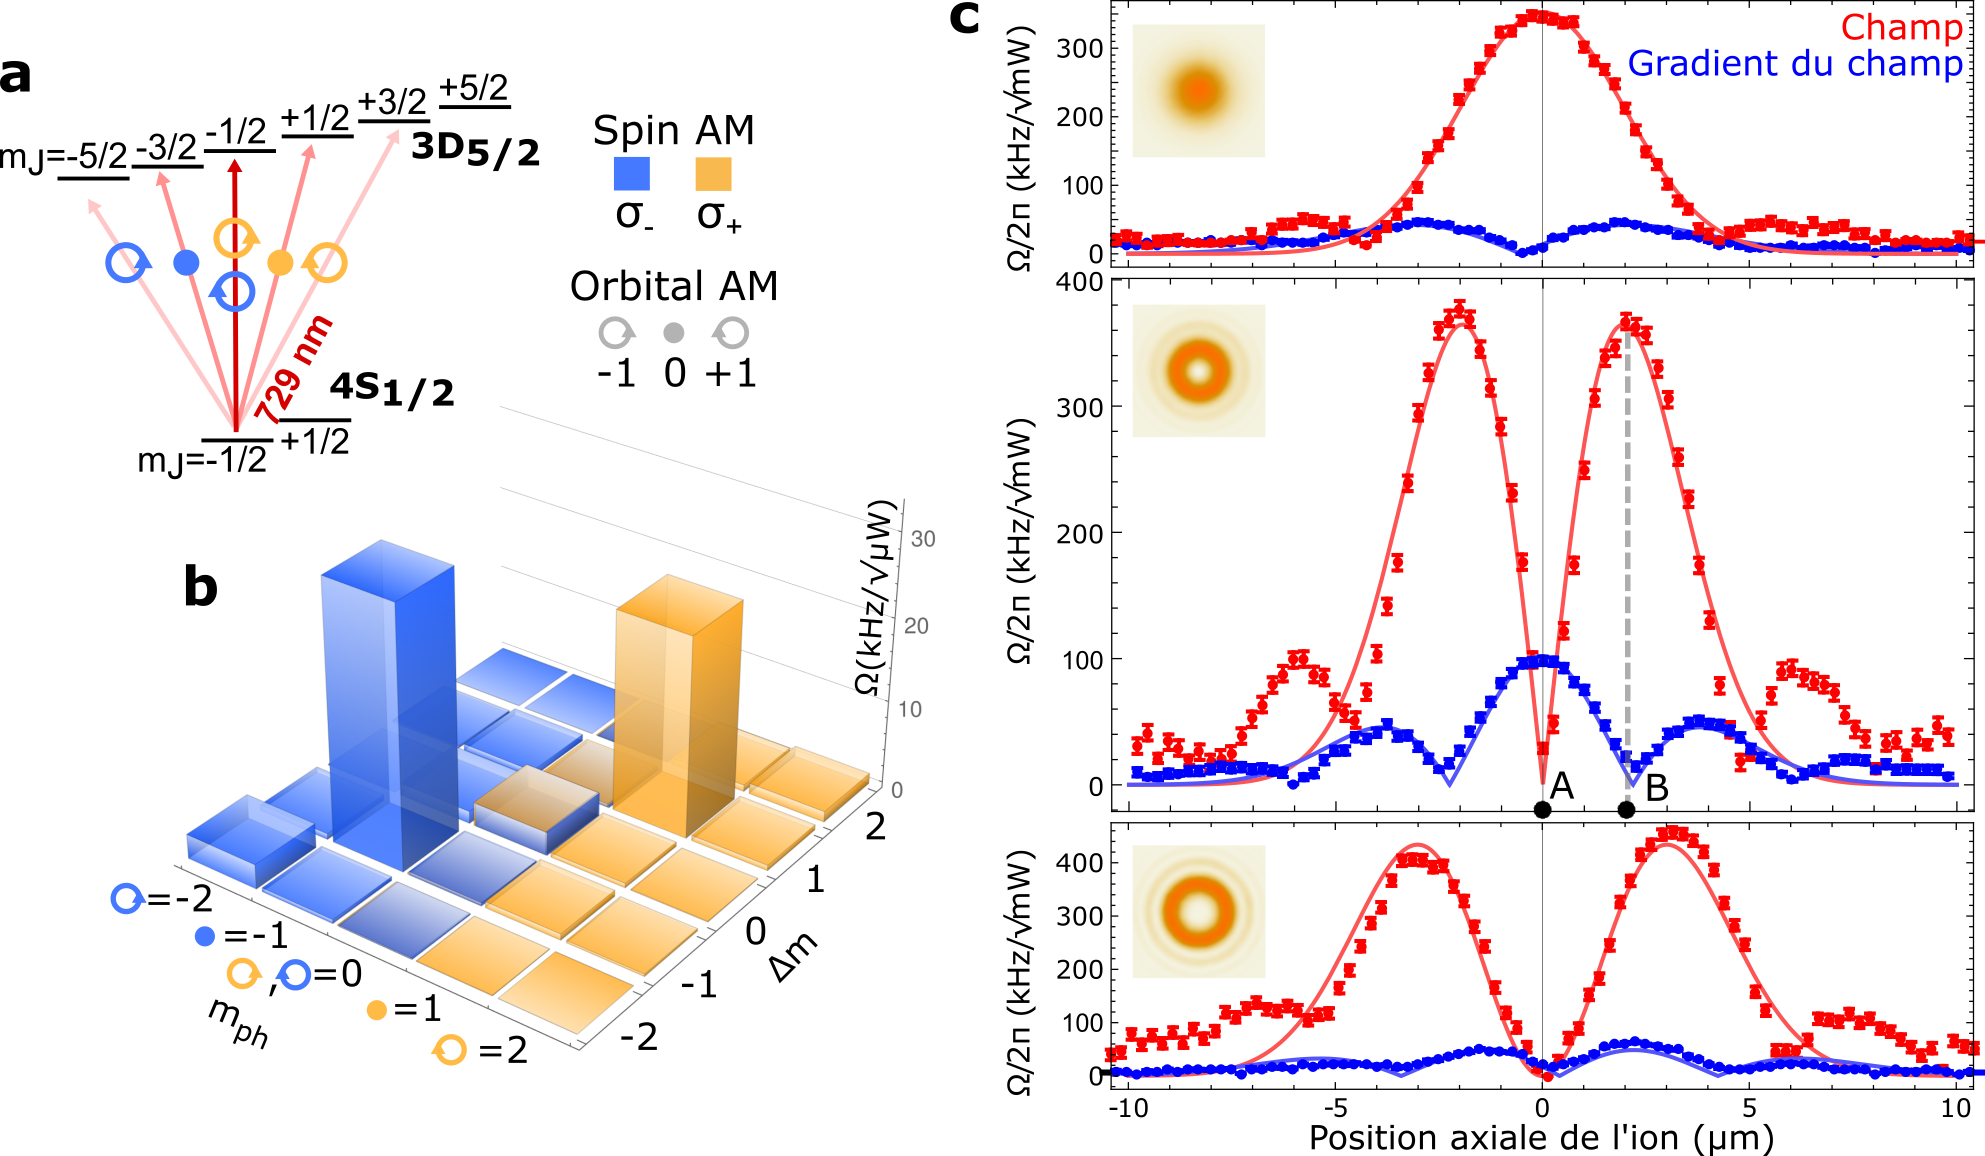
\includegraphics[width=0.9\columnwidth]{Figures/schmiegelow.png}
\caption{Observation de transition quadripolaire. (a) Transitions possibles mettant en jeu le MAS et le MAO. (b) Amplitudes de transition mesurées en utilisant une oscillation de Rabi. (c) Amplitude de transition dipolaire (rouge) et quadripolaire (bleu) en fonction de la position transverse de l'ion. Ces amplitudes sont reliées respectivement à l'amplitude du champ et du gradient du champ.}
\label{Fig:Schmiegelow}
\end{figure}


Nous avons maintenant terminé cette partie sur le concept de moment angulaire de la lumière. Nous avons introduit les définitions nécessaires et construit des champs électromagnétiques réalisables en pratiques dans lesquelles le moment angulaire est contrôlé. Dans le chapitre III, nous étudierons expérimentalement la génération de modes de Laguerre-Gauss à partir d'un laser infrarouge Gaussien, avant d'utiliser ces modes pour générer des harmoniques d'ordre élevé. Dans le chapitre IV, nous nous intéresserons au cas du moment angulaire de spin, c'est-à-dire de faisceaux polarisés circulairement. Nous chercherons à générer des harmoniques d'ordre élevé polarisées circulairement et à les utiliser dans l'étude de molécules chirales.
%\chapter{Le moment angulaire orbital dans la génération d'harmoniques d'ordre élevé}
\label{CH:OAM_HHG}
%
\section{Revue des utilisations pratiques des modes de Laguerre-Gauss}
\subsection{Le domaine visible et infrarouge}
\subsection{De plus courtes longueurs d'ondes : perspectives d'applications dans l'extrême ultra-violet}
\subsection{Des durées ultra-brèves : utilisations possibles d'impulsions attosecondes portant du moment angulaire orbital}

\section{Génération d'harmoniques d'ordre élevé à partir de modes de Laguerre-Gauss}

Ayant passé en revue les utilisations envisagées de faisceaux de Laguerre-Gauss de durées ultra-brève et dans le domaine de l'extrême ultra-violet (XUV), nous décrirons ici comment les générer de manière expérimentale. Nous commencerons par détailler notre dispositif de génération d'harmoniques d'ordre élevé dans le cas habituel d'un mode laser Gaussien, puis expliquerons comment passer au cas Laguerre-Gaussien avant de donner les résultats obtenus.

\subsection{Le cas Gaussien : Aspects expérimentaux de la génération d'harmoniques d'ordre élevé}
\label{Sec:HHG_G}
\subsubsection{Système laser}
Toutes les expériences présentées dans ce chapitre ont été réalisées sur le laser LUCA (Laser Ultra-Court Accordable) du LIDYL au CEA Saclay. Il délivre des impulsions ayant une enveloppe temporelle gaussienne de largeur à mi-hauteur $\tau = 50$ fs et une enveloppe spatiale gaussien de largeur à mi-hauteur $w_0 = 15$ mm à $\frac{1}{e^2}$. La longueur d'onde utilisée est 800 nm, et le taux de répétition est de 20 Hz. Ce système dispose d'une fibre utilisée pour filtrer spatialement le faisceau, ce qui garantit un profil très proche d'un mode gaussien pur \mycite{MahieuAPB2015}. Le prix à payer est une diminution de l'énergie par impulsion, qui atteint quand même environ 35 mJ après la fibre et le dernier étage de compression.

\subsubsection{Génération d'harmoniques d'ordre élevé}
Nous commençons par mettre en forme le faisceau laser : son diamètre est ajusté à l'aide d'un iris et son énergie est ajustée grâce à un atténuateur constitué d'une lame demi-onde et d'une paire de polariseur croisés. \`{A} la sortie de cet atténuateur, la polarisation du laser est verticale (S). Le faisceau est ensuite focalisé par une lentille dans un jet de gaz délivré par une vanne pulsée à la fréquence du laser par un système piezo-électrique (Attotech). L'utilisation d'une vanne pulsée permet de n'envoyer du gaz que lorsque le faisceau laser est présent, ce qui limite la pression résiduelle dans les chambres à vide. Ainsi, on peut atteindre une pression assez élevé (XXX) dans la région focale sans que l'émission harmonique ne soit réabsorbée par le gaz résiduel. Un autre paramètre important est le diamètre de l'orifice de la vanne (ici, 150 $\mu m$) : en choisissant un diamètre faible, on crée une extension supersonique du gaz ce qui garantit une longueur d'interaction faible avec le laser. On s'approche ainsi des conditions idéales d'un plan d'atomes, ce qui limite l'importance des effets d'accord de phase dans la GHOE. \par
Le choix du gaz dépend de l'expérience réalisée : on peut par exemple utiliser une molécule dont on étudie la réponse, on parle alors de spectroscopie harmonique. Le gaz n'est pas l'objet d'étude dans notre cas, on préférera donc choisir un système simple, facile à se procurer, et ayant une grande section efficace. Le gaz le plus courant est l'Argon, qui est peu coûteux et génère de manière très efficace. Son potentiel d'ionisation est de 15.76 eV, ce qui donne une énergie de coupure assez faible et qui empêche de générer des ordres harmoniques très élevés. Dans les cas où on désire générer des ordres élevés et nombreux, on pourra utiliser d'autres gaz rares comme le Néon ($I_p$ = 21.6 eV) même si la génération sera moins efficace.

Pour notre système, les paramètres nominaux sont :
\begin{itemize}
\item Le diamètre avant focalisation \O{} $\approx$ 10-15 mm,
\item L'énergie par impulsion de l'ordre de E = 1 mJ,
\item La lentille de longueur focale f = 1 m. \\
\end{itemize}
Pour calculer la valeur de l'intensité pic au foyer, on peut calculer le profil du faisceau après focalisation, par exemple par un calcul numérique. Le champ avant la lentille est défini dans les coordonnées cylindriques $(R,\theta)$ par :
\begin{equation*}
E(R,\theta) = \sqrt{I_0} \exp{\left(-\frac{R^2}{w_0^2}\right)}\times\delta(\frac{\mbox{\O}}{2}-R),
\end{equation*}
où $w_0$ est la largeur du faisceau collimaté avant l'iris, \O{}  est le diamètre de l'iris, $\delta$ est la fonction de Heaviside, et $I_0 = \frac{2E\sqrt{\frac{4\log{2}}{\pi}}}{\tau\pi w_0^2}$.
La focalisation d'un faisceau par une lentille mince peut être calculée par une transformée de Fourier (voir \mycite{Goodman}, un des ouvrages de référence pour l'optique de Fourier, et \mycite{Tan} pour des exemples d'implémentations numériques). Il est alors simple de voir l'effet des différents paramètres expérimentaux. Par exemple, on peut faire varier le diamètre de l'iris : la Figure \ref{Fig:IrisScan} montre le profil du faisceau au foyer quand \O{} varie entre 5 et 25 mm. On voit alors que l'intensité pic au foyer évolue entre 0 et 10 $\times 10^{14} \mbox{W/cm}^2$. On se trouve donc parfaitement dans le régime d'intensité nécessaire à la génération d'harmonique : l'intensité est suffisante pour enclencher une ionisation tunnel mais reste assez faible pour ne pas ioniser et dépléter tout le milieu.

\begin{figure}[!ht]
\centering
\def\svgwidth{\columnwidth}
\import{Figures/Iris_Scan/}{Fig_IrisScan.pdf_tex}
\caption{\'{E}volution du foyer lorsqu'on varie la taille de l'iris. De gauche à droite : (1) profil transverse de l'intensité au foyer, (2) intensité pic, (3) taille du waist. Les paramètres sont les suivants : E = 1 mJ, $w_0$ = 15 mm, $\tau$ = 50 fs, $\lambda$ = 792 nm, f = 1 m et \O{} variant de 5 à 25 mm par pas de 1 mm. Le calcul est réalisé sur une grille de 1025x1025 points correspondant à une taille réelle de 5*\O{}.}
\label{Fig:IrisScan}
\end{figure}

Les harmoniques d'ordre élevé du laser infrarouge sont ainsi générées par le gaz situé près du foyer de la lentille. Ce rayonnement XUV est ensuite ré-imagé par un dispositif composé de deux optiques :
\begin{enumerate}
\item Un miroir torique en or de 50 cm de focale. Le miroir travaille à $11.5\degres$ d'incidence rasante ($78.5\degres$ si on défini l'angle par rapport à la normale au miroir), ce qui permet d'avoir une réflectivité importante et plate sur la gamme spectrale considérée (voir Figure \ref{Fig:TorR}).

\begin{figure}[!ht]
\centering
\def\svgwidth{0.6\columnwidth}
\import{Figures/Reflect_Torique/}{torR.pdf_tex}
\caption{Réflectivité calculée du miroir torique en or à un angle d'incidence de $11.5\degres$. (CXRO, \mycite{Henke1993}).}
\label{Fig:TorR}
\end{figure}

Le miroir toroïdal est positionné dans une configuration 2f-2f de sorte à garder un rapport 1:1 entre le foyer de génération et le second foyer. Ré-imager le foyer de génération est utile car on peut focaliser le rayonnement harmonique dans un deuxième dispositif, comme par exemple un spectromètre à temps de vol dans le cas d'une mesure RABBIT (voir ChapitreXX et YY). Un autre avantage est qu'il éloigne la zone de génération, où la pression est élevée, de la zone de détection, qui requiert souvent un vide de qualité pour que les détecteurs fonctionnent.\\

\item La deuxième optique est une lame de Si$\mbox{O}_{\mbox{2}}$, qui réalise le rôle de filtrage de l'infrarouge de génération. La lame de silice est traitée antireflet pour l'infrarouge grâce à un dépôt de multicouches. La dernière de ces couches est en silice, ce qui combiné à une bonne qualité de surface permet de réfléchir efficacement le rayonnement harmonique. La Figure \ref{Fig:SilR}, tirée de \mycite{MairessePhD} présente la réflectivité de la lame pour le rayonnement harmonique et infrarouge. La réflectivité dans l'XUV est donc supérieure à 50\% jusqu'à l'ordre $\approx 37$, tandis que moins de 10\% de l'infrarouge est réfléchi. Le filtrage de l'infrarouge de génération est souvent crucial : il constitue un bruit de mesure non négligeable, sans compter qu'il peut facilement endommager des optiques ou des détecteurs en aval s'il est focalisé.

\begin{figure}[!ht]
\centering
\def\svgwidth{\columnwidth}
\import{Figures/Reflect_Silice/}{silR.pdf_tex}
\caption{Réflectivité de la lame de silice. \`{A} gauche, transmission et réflectivité à 800 nm en fonction de l'angle d'incidence rasante. Les pointillés repèrent notre angle de $11.5\degres$. \`{A} droite, réflectivité XUV mesurée (cercles) et donnée par le CXRO (lignes) (\mycite{Henke1993}). Figure adaptée de \mycite{MairessePhD}.}
\label{Fig:SilR}
\end{figure}
\end{enumerate}

Nous souhaiterions ensuite pouvoir imager le spectre harmonique, c'est-à-dire séparer les différents ordres harmoniques et mesurer leurs propriétés spatiales. Un peu après le second foyer, les harmoniques sont dispersées par un réseau à pas variable Hitachi 001-0437 (voir \mycite{KitaAO1983} pour des détails sur son fonctionnement). L'angle de réflexion d'un rayonnement monochromatique de longueur d'onde $\lambda$ est donné par la formule des réseau :
\begin{equation*}
m\lambda=\frac{\sin{\alpha}+\sin{\beta}}{\sigma},
\end{equation*}
où $m$ est l'ordre de diffraction considéré (généralement 1), $\sigma$ le nombre de trait par mètre (1200 traits/mm dans notre cas), $\alpha$ et $\beta$ les angles d'incidence et de réflexion, définis par rapport à la normale au réseau (la documentation donne $\alpha = 87$\degres{} pour un fonctionnement optimal).\par
Le réseau de diffraction est cylindrique : il est focalisant dans la dimension horizontale mais est plan dans la direction verticale. Un rayonnement gaussien de faible largeur spectrale $\Delta\lambda$ et de largeur spatiale $w(z)$ formera donc dans le plan focal du réseau une fine ligne verticale de largeur proportionnelle à $\Delta\lambda$ et de hauteur $w(z)$. On image ainsi à la fois les dimensions spectrale et spatiale, si on suppose la symétrie cylindrique. Ce spectre est imagé par des galettes de micro-canaux couplées à un écran de phosphore, lui-même observé par une caméra CCD Basler A102f. 

L'intégralité du dispositif expérimental est représenté sur la Figure \ref{Fig:ExpG}.
\newpage
\vspace{\baselineskip}
\begin{figure}[!ht]
\centering
\def\svgwidth{\columnwidth}
\import{Figures/Setup_G/}{setupG_wbitmap.pdf_tex}
\caption{Dispositif expérimental de génération et détection d'harmoniques d'ordre élevé.}
\label{Fig:ExpG}
\end{figure}

Les figures \ref{Fig:SpectrumGAr} et \ref{Fig:SpectrumGNe} présentent des spectres obtenus avec ce dispositif en utilisant respectivement l'argon et le néon comme gaz de génération. On observe les ordres harmoniques allant de 13 à 29 dans l'argon, et de 13 à 57 dans le néon, la différence d'énergie de coupure étant attendue puisque le néon a un $I_p$ plus élevé. Sur le spectre de l'argon, on observe clairement les deux trajectoires quantiques de la GHOE : une contribution sur l'axe correspond à la trajectoire courte et une plus divergente et moins intense correspond à la trajectoire longue. Dans le cas du néon, les conditions d'accord de phase utilisées favorisent la trajectoire courte. On remarque également que la divergence de la trajectoire courte (resp. longue) augmente (rep. diminue) avec l'ordre harmonique, jusqu'à ce que les deux trajectoires se confondent dans la coupure. Notons finalement la présence sur le spectre du néon de pics satellites autour des harmoniques les plus basses : il s'agit des harmoniques plus élevées diffractées au second ordre par le réseau.
\begin{figure}[!ht]
\centering
\def\svgwidth{\columnwidth}
\import{Figures/Spectrum_G/}{Spectrum_G_Ar.pdf_tex}
\caption{Spectre d'harmoniques d'ordre élevé générées dans l'argon à partir d'un mode laser gaussien.}
\label{Fig:SpectrumGAr}
\end{figure}
\begin{figure}[!ht]
\centering
\def\svgwidth{\columnwidth}
\import{Figures/Spectrum_G/}{Spectrum_G_Ne.pdf_tex}
\caption{Spectre d'harmoniques d'ordre élevé générées dans le néon à partir d'un mode laser gaussien.}
\label{Fig:SpectrumGNe}
\end{figure}

\subsection{Génération de modes de Laguerre-Gauss dans le visible et proche infrarouge}
Ayant décrit la génération ``habituelle'' d'harmoniques d'ordre élevé, décrivons maintenant l'expérience où le laser générateur possède un mode de Laguerre-Gauss, dont l'expression a été donnée au chapitre précédent (équation \ref{eq:lgmodes}). Les modes de Laguerre-Gauss possèdent un moment angulaire orbital bien défini grâce à leur phase hélicoïdale. Plus précisément, c'est le terme $e^{\rmi\ell\theta}$, également présent dans les modes de Bessel, qui leur confère cette propriété. Il sera question de l'index radial $p$ des modes de Laguerre-Gauss plus loin dans cette thèse, mais il n'a pour l'instant pas d'importance pour notre problème. La première question est donc de savoir comment produire un mode de Laguerre-Gauss d'index $(\ell_{IR},0)$ dans l'infrarouge. 

\subsubsection{Superposition de modes de Hermite-Gauss}
\label{sec:hg_modes}
Les faisceaux de LG étant des modes du champ électromagnétique, on peut d'abord penser à modifier le laser lui-même pour qu'il lase directement dans le mode désiré. En introduisant des éléments absorbants dans la cavité, il est a priori possible d'interdire la génération d'un mode Gaussien. En pratique, il est assez compliqué de sélectionner un mode de LG. Il est par contre assez simple de sélectionner un des modes de \textit{Hermite-Gauss}, qui sont les solutions de l'équation d'onde en coordonnées cartésiennes. Ces modes sont souvent appelés modes $\mbox{TEM}_{nm}$, pour ``Transverse Electro-Magnetic'', dont le mode Gaussien $\mbox{TEM}_{00}$ n'est simplement que le mode d'index le plus bas. Quelques uns de ces modes sont représentés sur la figure \ref{Fig:hgmodes}. En insérant simplement un fil vertical (resp. horizontal) dans la cavité laser, on bloque la génération du $\mbox{TEM}_{00}$ et on obtient un mode $\mbox{TEM}_{01}$ (resp. $\mbox{TEM}_{10}$).

\begin{figure}[!ht]
\centering
\def\svgwidth{\columnwidth}
\import{Figures/Mode_Converter/}{HG_Modes.pdf_tex}
\caption{Modes de Hermite-Gauss pour différentes valeurs de $(n,m)$. De gauche à droite, $(n,m) =$ (0,0), (1,0), (0,1), (2,0), (2,1), (3,3). Le code couleur est le même que celui de la figure \ref{Fig:LGModes} : la couleur donne la phase et la luminosité l'intensité.}
\label{Fig:hgmodes}
\end{figure}

Les faisceaux de Hermite-Gauss constituent également une base des modes du champ, dans laquelle on peut donc écrire les modes de Laguerre-Gauss. On peut montrer (\mycite{BeijersbergenOC1993}) que les composantes du mode $\mathcal{LG}_{\ell,p}$ sont égales aux composantes d'un mode $\mbox{TEM}_{nm}$ incliné à 45\degres{} avec $p = \mathrm{min}(m,n)$ et $\ell=m-n$, la seule différence étant l'ajout d'une phase de $\pi/2$ entre les différentes composantes successives. Par exemple pour $\ell = 1$,
\begin{align*}
\mbox{TEM}_{n,m}^{45\mbox{\degres}}&=\frac{1}{\sqrt{2}}\mbox{TEM}_{01}+\frac{1}{\sqrt{2}}\mbox{TEM}_{10} \mbox{ et}\\
\mathcal{LG}_{1,0}&=\frac{1}{\sqrt{2}}\mbox{TEM}_{01}+\frac{\rmi}{\sqrt{2}}\mbox{TEM}_{10}.
\end{align*}
Pour $\ell = 2$, 
\begin{equation*}
\mathcal{LG}_{2,0}=\frac{1}{2}\mbox{TEM}_{02}+\frac{\rmi}{\sqrt{2}}\mbox{TEM}_{11}-\frac{1}{\sqrt{2}}\mbox{TEM}_{20}
\end{equation*}
et ainsi de suite.
Comme dit plus haut, il est possible de générer un mode $\mbox{TEM}_{n,m}$ en cavité, il reste seulement à l'incliner à 45\degres par rapport au repère choisi. Pour contrôler la phase entre les composantes relatives, les auteurs de \mycite{BeijersbergenOC1993} ont montré qu'on pouvait utiliser des lentilles cylindriques. En effet, une lentille cylindrique convergente ne focalise qu'une seule des composantes cartésiennes, qui va subir un déphasage au passage du foyer dû à la phase de Gouy. On recollimate ensuite le faisceau avec une deuxième lentille cylindrique de même focale $f$. La phase ajoutée est ajustée en changeant la distance entre ces deux lentilles; pour obtenir $\pi/2$ il faut choisir $\sqrt{2}f$. La Figure \ref{Fig:Modeconv} illustre le principe de ce dispositif, appelé convertisseur de mode.

\begin{figure}[!ht]
\centering
\def\svgwidth{0.5\columnwidth}
\import{Figures/Mode_Converter/}{mode_converter.pdf_tex}
\caption{Schéma de fonctionnement d'un convertisseur de mode : en partant d'un $\mbox{TEM}_{01}$ incliné à 45\degres, on obtient un mode $\mathcal{LG}_{1,0}$. Tiré de \mycite{PadgettAllen1999}.}
\label{Fig:Modeconv}
\end{figure}

L'intérêt de ce dispositif est de créer des modes purs : on obtient exactement le faisceau de Laguerre-Gauss recherché. Il présente cependant deux inconvénients : (1) il faut disposer d'un mode $\mbox{TEM}_{0\ell}$ au départ, ce qui devient compliqué dès que $\ell$ augmente. De plus, il est peu pratique de devoir modifier la cavité laser, particulièrement dans le cas des lasers de puissances utilisés pour la HHG. (2) Le faisceau est focalisé dans une dimension entre les deux lentilles. La puissance fournie par notre laser imposerait de réaliser la conversion dans une enceinte à vide, sans quoi la focalisation dans l'air détruira le profil spatial et temporel du faisceau. Pour ces raisons, nous avons choisi une méthode plus flexible et plus adapté à un laser de puissance.

\subsubsection{Utilisation d'une lame de phase à spirale}
Cette technique est probablement la façon la plus intuitive d'ajouter le terme de phase qui nous intéresse au faisceau. Pour rajouter une phase $e^{\rmi\ell\theta}$, il suffit d'utiliser une lame de verre transparente dont l'épaisseur varie proportionnellement à $\theta$. On forme ainsi une \textit{lame de phase à spirale} (Spiral Phase Plate, SPP), concept proposé dans \mycite{BeijersbergenOC1994} et représenté sur la Figure \ref{Fig:SPP}.\par
\begin{figure}[!ht]
\centering
\def\svgwidth{0.5\columnwidth}
\import{Figures/SPP/}{SPP.pdf_tex}
\caption{Lame de phase à spirale. La flèche rouge représente le trajet d'un rayon optique. Adapté de \mycite{YaoAOP2011}.}
\label{Fig:SPP}
\end{figure}
La lame présente une discontinuité pour $\theta=0$\degres, dont la hauteur h permet de contrôler le moment angulaire orbital transféré au faisceau pour une longueur d'onde donnée. Si cette hauteur est assez faible pour que l'on reste dans le régime paraxial, on peut considérer que la lame agit uniquement sur la phase du faisceau incident. Ainsi si on choisit 
\begin{equation*}
h = \frac{\ell\lambda}{n-1},
\end{equation*}
où $n$ est l'indice de réfraction du milieu, pour un champ d'entrée $u(r,\theta,z)$ on obtient directement après la lame $u' = u\exp{(-\rmi \ell \theta)}$.	Il est donc non seulement possible de passer d'un mode Gaussien à un mode Laguerre-Gaussien, mais encore de changer l'indice d'un mode déjà Laguerre-Gaussien.\par
La lame de phase illustre joliment la création de MAO : si on considère une onde plane arrivant perpendiculairement à la surface plane de la lame, le rayon qui sort de la lame sera dévié par réfraction à travers la surface hélicoïdale. Cette réfraction se fait dans la direction azimutale, le moment linéaire de la lumière acquière donc une composante azimutale, synonyme de moment angulaire. Plus précisément, pour un rayon $r$ donné, l'angle de la surface	vaut $h/(2\pi r)$. Si on applique la loi de Snell-Descartes on obtient que le rayon est dévié d'un angle $\alpha = (n-1)\ell\lambda/(2\pi r(n-1)) = \ell/(k_0r)$. Le moment linéaire par photon vaut $\hbar k_0$, donc le moment angulaire par photon vaut $r\times\hbar k_0\times\ell/(k_0r) = \ell\hbar$.


Si le principe d'une SPP est simple, sa construction est beaucoup plus compliquée. Les tolérances sur la valeur de h et la régularité de la surface sont très strictes aux longueurs d'ondes optiques, sans quoi la qualité du mode de sortie sera détériorée (si h n'est pas adapté, on peut même créer des modes d'indice non entier, cf. \mycite{LeachNJP2004}). D'ailleurs, lors des premiers travaux sur le sujet (\mycite{BeijersbergenOC1994}), la température de la lame était ajustée pour accorder précisément la hauteur de la lame à la longueur d'onde. La technique a évolué et il est maintenant possible de créer des SPP de très bonne qualité \mycite{OemrawsinghAO2004}.

Enfin, remarquons que même pour une SPP parfaite, la conversion d'un mode à l'autre n'est jamais idéale. La SPP agit sur la phase du faisceau, mais ne modifie pas le profil d'intensité. Ainsi, à sa sortie le champ électrique a la bonne phase mais pas la distribution d'intensité d'un mode de Laguerre-Gauss (termes sur la première ligne de l'équation \ref{eq:lgmodes}). La conséquence est que le champ $u_{exp}$ créé n'est pas un mode pur du champ, mais une superposition de modes de Laguerre-Gauss de différents indices. Ainsi, son intensité sera fortement modulée au cours de la propagation selon la phase entre ces différents modes. Le cas qui nous intéresse principalement est la conversion d'un mode Gaussien vers un mode LG. Dans ce cas, cette superposition s'écrit :
\begin{align}
\begin{split}
u_{exp}(r,\theta,z) &= \sum_{p=0}^\infty\sum_{\ell=-\infty}^\infty{\Braket{u_{exp}(r,\theta,z)|\mathcal{LG}_{\ell,p}(r,\theta,z)} \ket{\mathcal{LG}_{\ell,p}(r,\theta,z)}}\\
&=\sum_{p=0}^\infty\sum_{\ell=-\infty}^\infty{\Braket{TEM_{00}(r,\theta,z)\cdot e^{\rmi\ell'\theta}|\mathcal{LG}_{\ell,p}(r,\theta,z)} \ket{\mathcal{LG}_{\ell,p}(r,\theta,z)}},
\end{split}
\label{Eq:decompLG}
\end{align}
où $\ell'$ est l'indice azimutal correspond à la hauteur de la SPP. Les coefficients sont simplement donnés par le produit scalaire ci-dessus. On remarque qu'il a la forme suivante :
\begin{equation*}
\Braket{TEM_{00}(r,\theta,z)\cdot e^{\rmi\ell'\theta}|\mathcal{LG}_{\ell,p}(r,\theta,z)} = \int_{r=0}^\infty\int_{\theta=0}^{2\pi}{\ldots \; e^{\rmi(\ell'-\ell)\theta}r\rmd r \rmd \theta},
\end{equation*}
l'intégrale selon $\theta$ s'annule donc dès que $\ell\neq\ell'$. Les modes de la superposition ont donc tous le même index azimutal mais des $p$ différents. Ces coefficients peuvent être calculés numériquement, par exemple \mycite{BeijersbergenOC1994} obtiennent pour le cas $\ell' = 1$ les valeurs présentées dans le Tableau \ref{Tab:DecompBei}. On conclut donc que le faisceau est composé majoritairement du mode $\mathcal{LG}_{1,0}$. Les valeurs deviennent moins bonne lorsqu'on augmente $\ell$, par exemple un Gaussien passant à travers une lame dessinée pour ajouter $\Delta\ell =2$ n'est composé qu'à 50\% du mode $\mathcal{LG}_{2,0}$ recherché.
\begin{center}
  \begin{tabular}{ c | c | c | c | c | c | c }
    \hline
		& $p = 0$ & 1 & 2 & 3 & 4 & 5 \\ \hline
    $\ell=1$ & 78.5 & 9.82 & 3.68 & 1.92 & 1.17 & 0.79 \\ \hline
  \end{tabular}
	\caption{Décomposition du champ obtenu en passant un mode Gaussien pur à travers une lame de phase à spirale. D'après \mycite{BeijersbergenOC1994}.}
	\label{Tab:DecompBei}
\end{center}
Pour finir, mentionnons une technique permettant de relâcher un peu les contraintes de fabrication d'une SPP : il est possible de discrétiser la pente de phase, ce qui rend la lame plus facile à construire et donc plus accessible. Cette technique est détaillée dans \mycite{SuedaOE2004}, où les auteurs calculent l'influence du nombre de points de discrétisation sur la pureté modale obtenue :
\begin{center}
  \begin{tabular}{c | c | c | c | c | c}
    \hline
		Nombre de points de discrétisation & $\infty$ & 32 & 16 & 8 & 4 \\ \hline
    Efficacité $\mathcal{LG}_{0,0}\rightarrow\mathcal{LG}_{1,0}$ & 78.5 & 78.3 & 77.5 & 74.6 & 63.7 \\ \hline
  \end{tabular}
	\caption{Efficacité de conversion d'une lame de phase à spirale $\Delta\ell=1$ en fonction du niveau de discrétisation. D'après \mycite{SuedaOE2004}.}
	\label{Tab:DecompSueda}
\end{center}
La qualité du mode obtenue est donc très correcte même jusqu'à 8 niveaux. Les auteurs montrent également que ces lames de phase sont adaptées à des utilisations avec des faisceaux courts et intenses, contrairement à la plupart des autres méthodes. Pour ces raisons, nous avons finalement choisi d'utiliser une lame de phase discrétisée sur 16 niveaux, et disposons de lames $\Delta\ell = 1$ et $\Delta\ell = 2$ à 800 nm, ce qui nous permet d'aller jusqu’à $\ell = 3$ en les mettant l'une après l'autre.

\subsubsection{Résultats expérimentaux sur la création de modes de Laguerre-Gauss dans l'infrarouge}
Même si le système laser a été décrit plus haut, notons encore une fois l'importance du filtrage spatial installé sur notre chaîne : il nous garantit un mode Gaussien très pur, ce qui favorise grandement la création de modes Laguerre-Gaussien de qualité. \par
Les lames de phases utilisées ont été construites par la société Silios Technologies et font 17 mm de diamètre. Elle ou elles sont insérées directement après l'iris et avant la lentille. Le faisceau étant bien collimaté, nous n'avons pas observé de différence notable selon le placement de la lame. Il est intéressant d'observer l'intensité du faisceau un peu après le passage dans la lame : 

\begin{figure}[!ht]
\centering
\def\svgwidth{0.4\columnwidth}
\import{Figures/SPP/}{Beam_1m_After_SPP.pdf_tex}
\caption{Intensité transverse après être passée dans une lame de phase à spirale $\Delta\ell = 1$. Le faisceau est d'abord diaphragmé par un iris de diamètre 10 mm, la distance d'observation après la lame est de 1 m.}
\label{Fig:BeamAfterSPP}
\end{figure}

On observe 16 ``pétales'' sur les bords du faisceau, qui correspondent à la diffraction par les 16 marches de la lame. On voit également la singularité de phase déjà formée, qui donne un zéro d'intensité au centre. Clairement, l'intensité du faisceau est encore très loin de celle d'un mode de Laguerre-Gauss : il n'y a que dans le champ lointain que le faisceau prendra la forme désirée. Dans notre cas, cela se passe au foyer de la lentille de génération. Nous imageons ce foyer à l'aide d'une caméra CCD Imagine Source équippée d'un objectif x5 et d'un tube de 160 mm. La figure \ref{Fig:LGFocus} présente les résultats obtenus.\par
\begin{figure}[!ht]
\centering
\def\svgwidth{0.8\columnwidth}
\import{Figures/IRFocus/}{SPP1focus.pdf_tex}
\caption{Intensité laser au foyer d'une lentille de 1m, après passage à travers (1) une lame de phase $\Delta\ell = 1$, (2) une lame de phase $\Delta\ell = 2$, et (3) les deux lames placées successivement.}
\label{Fig:LGFocus}
\end{figure}
On mesure le diamètre de l'anneau, défini comme la distance entre les deux maxima d'intensité le long d'une ligne radiale, et on obtient 200, 280 et 400 \si{\um} pour $\ell=$1, 2, 3. Ceci est cohérent avec la dépendance en $\sqrt{\ell}$ attendue (voir équation \ref{Eq:rmax_LG}), mais ne constitue pas une mesure directe du MAO porté par le faisceau. Pour ce faire, il existe de nombreuses techniques développées dans le domaine visible et infrarouges dont le but est toujours de révéler le terme de phase $\mathrm{e}^{\rmi\ell\theta}$. Pour révéler cette phase spatiale, il est naturel d'essayer d'observer des interférences, soit avec un autre faisceau - l'interférence avec un gaussien donne une ``fourche'' d'ordre $\ell$ \mycite{bazhenov1990} - ou bien du faisceau avec lui même, c'est-à-dire sa diffraction. De nombreux objets diffractifs ont été utilisés, par exemple une fente \mycite{ghai2009} ou des fentes de Young \mycite{sztul2006}, avec lesquelles le signe et la parité de $\ell$ se retrouvent dans le décalage des franges, ou bien des objets plus compliqués tels que des grilles de pupilles \mycite{berkhout2008} qui donnent directement la valeur de $\ell$. On peut également mentionner les ouvertures bloquant une partie angulaire du faisceau, ce qui se répercute sur le contenu modal du faisceau à travers la relation d'incertitude $\Delta\ell\Delta\phi > K$ déjà mentionnée (TODO). Certaines méthodes sont généralisables au cas d'un photon unique et ont permis de mesurer de l'intrication entre différents états de moment orbital angulaire \mycite{MairNature2001} ainsi qu'un équivalent angulaire au paradoxe EPR \mycite{LeachScience2010}. \par 
Nous avons choisi d'utiliser une ouverture en triangle, qui donne une figure de diffraction assez surprenante : on obtient une grille de points diffractés en forme de triangle, dont l'orientation donne le  signe de $\ell$ alors que le nombre de points donne $\left|\ell\right|$ : sur l'arête extérieure au triangle, on a $\left|\ell\right|+1$ points \mycite{HickmannPRL2010}. Après être passé dans la SPP, le faisceau est diffracté par une ouverture triangulaire dont la taille est ajustable à l'aide d'un système motorisé conçu par M. Bougeard. On choisit l'ouverture de l'ordre du waist du faisceau, ce qui permet d'observer la figure de diffraction en imageant le foyer d'une lentille de focale f=1m. La figure \ref{Fig:Triangle} illustre le principe et les résultats de cette expérience. 

\begin{figure}[!ht]
\centering
\def\svgwidth{1.0\columnwidth}
\import{Figures/Triangle/}{triangle.pdf_tex}
\caption{Mesure directe du moment angulaire orbital porté par le faisceau infrarouge à l'aide d'une ouverture triangulaire.}
\label{Fig:Triangle}
\end{figure}

Nous avons pu vérifier la validité de cette méthode pour des moments angulaires plus élevés. Pour les obtenir, le champ infrarouge $E_{800}$ est doublé à l'aide d'un cristal de BBO (bêta-borate de baryum). On obtient un champ à 400 nm, dont l'amplitude est donné par la loi habituelle de l'optique non-linéaire perturbative $E_{400}\propto E_{800}^2\propto \rme^{2\rmi\ell_{IR}\theta}$. Le MAO du faisceau est ainsi doublé, comme vérifié expérimentalement par \mycite{DholakiaPRA1996}. Les résultats obtenus après diffraction par la fente triangulaire sont présentés sur la figure \ref{Fig:Triangle400}. 

\begin{figure}[!ht]
\centering
\def\svgwidth{0.5\columnwidth}
\import{Figures/Triangle/}{triangle400.pdf_tex}
\caption{Mesure directe du moment angulaire orbital porté par le champ obtenu après doublage du faisceau infrarouge dans un cristal de BBO.}
\label{Fig:Triangle400}
\end{figure}

Ceci constitue donc une preuve directe que le faisceau est composé très majoritairement du mode $\mathcal{LG}_{\ell,0}$. Bien sûr, on ne s'attend quand même pas à ce que les modes obtenus soient purs, du fait de la lame de phase mais également à cause de l'iris qui limite la dimension transverse du faisceau. On peut évaluer numériquement l'effet de tous ces éléments : on effectue un calcul de propagation de la même façon qu'expliqué en page \pageref{Fig:IrisScan}, cette fois en rajoutant l'effet de la lame de phase discrète. Une fois le foyer obtenu, on calcule sa décomposition dans la base des modes de Laguerre-Gauss en évaluant numériquement les coefficients du type \ref{Eq:decompLG}. Comme noté page \pageref{Eq:rmax_LG}, les modes de Laguerre-Gauss ne constituent une base que pour une valeur de $w(z)$ donnée. Il faut donc choisir cette valeur avant d'effectuer la décomposition. On fait l'hypothèse que le mode obtenu est assez proche d'un mode pur $(\ell,0)$ pour que son rayon soit donné par l'équation \ref{Eq:rmax_LG}, ce qui nous permet de fixer $w(z)$. La figure \ref{Fig:DecompIR} montre l'intensité au foyer et les coefficients de la décomposition ainsi obtenus. On voit que le foyer est composé du mode $\mathcal{LG}_{\ell,0}$ à 72, 48 et 42\% pour $\ell=1,2,3$ respectivement. On observe également l'apparition d'un deuxième anneau pour $\ell =2$ et 3, dû au vignetage du faisceau par l'iris et cohérent avec la présence de davantage de modes $p$. \par

\begin{figure}[!ht]
\centering
\def\svgwidth{\columnwidth}
\import{Figures/Mode_Decomposition_IR/}{mode_L123.pdf_tex}
\caption{Intensité laser au foyer d'une lentille de 1m, après passage à travers (1) une lame de phase $\Delta\ell = 1$, (2) une lame de phase $\Delta\ell = 2$, et (3) les deux lames placées successivement.}
\label{Fig:DecompIR}
\end{figure}

Nous concluons donc que même si le contenu modal devient moins pur à mesure que $\ell$ augmente, le mode dominant reste celui qui nous intéresse. La GHOE étant un processus très non-linéaire, c'est lui qui contribuera majoritairement. 

\subsection{Génération d'harmoniques d'ordre élevé d'un faisceau de Laguerre-Gauss}
\subsubsection{Contraintes expérimentales}
Une fois qu'on dispose d'un faisceau infrarouge de MAO défini, l'expérience ne diffère en principe pas du cas Gaussien présenté dans la partie \ref{Sec:HHG_G}. En pratique, un problème important subsiste : celui de l'intensité pic. Nous avons vu que pour générer des harmoniques d'ordre élevé, l'intensité au foyer doit être de l'ordre de $\SI{1e14}{W/cm^2}$. Pour un mode de Laguerre-Gauss d'index $(\ell,0)$, l'intensité maximale est obtenue en $r_\mathrm{max}$ (équation \ref{Eq:rmax_LG}) :
\begin{align*}
I_\ell(r_\mathrm{max},z=0) &= \frac{C_{\ell,0}^2}{{w_0}^2}{\left( {\frac{r_\mathrm{max}\sqrt{2}}{{w_0}}} \right)^{2\left| \ell  \right|}}{e^{\left( { - \frac{{2{{r_\mathrm{max}}^2}}}{{{{w_0}^2}}}} \right)}}\\
&= \frac{2}{\pi(1+\delta_{0\ell})\left| \ell  \right|!{w_0}^2}\ell^{\left| \ell  \right|}{e^{-\ell}}
\end{align*}
La formule de Stirling donne $\left| \ell  \right|!\approx\sqrt{2\pi\left| \ell  \right|}\left| \ell  \right|^{\left| \ell  \right|}e^{-\left| \ell  \right|}$. Elle est valable respectivement à 8\%, 4\% et 2.6\% près pour $\ell=1,\;2,\;3$. On peut donc approximer :
\begin{equation*}
I_\ell(r_\mathrm{max},z=0) \approx \frac{2}{\pi{w_0}^2}\frac{1}{\sqrt{2\pi\left| \ell  \right|}}\text{ pour }\ell\neq0. 
\end{equation*}  
L'intensité pic évolue donc en $1/\sqrt{\left| \ell  \right|}$, la génération est donc de plus en plus compliquée à mesure que le MAO de l'infrarouge $\ell_{IR}$ augmente. Si on évalue l'expression exacte ci-dessus, on obtient :

\begin{center}
  \begin{tabular}{ c | c | c | c | c }
    \hline
		$\ell_{IR}$ & 0 & 1 & 2 & 3 \\ \hline
    $I_{\mathrm{max}}$ & 1 & 0.7358 & 0.5413 & 0.4481 \\ \hline
  \end{tabular}
	\caption{Intensité pic d'un mode de Laguerre-Gauss en fonction de $\ell$. Les intensités sont normalisées à celle du mode $\ell = 0$.}
\end{center}
Nous avons la chance de disposer d'un laser assez énergétique (jusqu'à 35 mJ disponibles), qui comme on le verra est suffisant pour générer jusqu'à $\ell_{IR}=3$. Il est égalemen

La seconde contrainte expérimentale est due au système d'imagerie. Comme démontré plus haut, le faisceau infrarouge est constitué d'un mode de Laguerre-Gauss principal. Le principe de conservation du moment angulaire nous amène à penser que les harmoniques générées doivent également porter du MAO, et prendront donc problablement la forme de modes de Laguerre-Gauss. Nous avons vu dans la partie \ref{sec:hg_modes} que les modes de Laguerre-Gauss peuvent être vus comme la superposition de plusieurs modes d'Hermite-Gauss et que le déphasage entre ces modes était crucial. En particulier, le convertisseur de mode présenté sur la figure \ref{Fig:Modeconv} repose sur l'utilisation de lentilles cylindriques pour contrôler la phase d'un seul des modes de Hermite-Gauss. On comprend donc que n'importe quel élément optique focalisant différemment les deux composantes cartésiennes du champ va modifier la phase relatives des modes HG et détruire le mode de Laguerre-Gauss. Dans notre dispositif présenté sur la figure \ref{Fig:ExpG}, on trouve deux éléments problématiques :
\begin{itemize}
\item Les optiques de focalisation peuvent être astigmatiques. En particulier, la lentille de focalisation et le miroir torique doivent être alignés parfaitement, sans quoi notre mode en sera perturbé.\\
\item Le réseau de diffraction du spectromètre est un réseau cylindrique, il va donc systématiquement détruire le profil du faisceau au passage de son foyer. 
\end{itemize}

L'effet du réseau de diffraction cylindrique peut être calculé. Par exemple, \mycite{VaityPLA2013} proposent d'utiliser l'astigmatisme introduit par une lentille inclinée pour mesurer le MAO porté par un faisceau. Nous adaptons ici leur formalisme au cas de notre réseau de diffraction. Considérons par simplicité un faisceau collimaté incident sur le réseau de diffraction. Pour décrire sa propagation, on peut utiliser les matrices de transfert. La matrice totale du système est
\begin{equation*}
M_{\mathrm{tot}} = M_{z_1}\cdot M_{\mathrm{r\acute{e}seau}}\cdot M_{z_0}\;,
\end{equation*}
où $z_0$ est la distance de propagation en amont du réseau, $z_1$ la distance en aval, $M_z$ et $M_{\mathrm{r\acute{e}seau}}$ décrivent respectivement la propagation sur une distance $z$ et la focalisation par le miroir :
\begin{equation*}
M_z = \left(
\begin{array}{cc}
	I & zI \\
	0 & I
\end{array} \right)\text{ avec } 
I = \left(
\begin{array}{cc}
	1 & 0 \\
	0 & 1
\end{array} \right)
\end{equation*}


\begin{equation*}
M_{\mathrm{r\acute{e}seau}} = \left(
\begin{array}{cc}
	I & 0 \\
	-C/f & I
\end{array} \right)\text{ avec } 
C = \left(
\begin{array}{cc}
	1 & 0 \\
	0 & 0
\end{array} \right).
\end{equation*}
$f$ est la longueur focale effective du réseau dans la direction horizontale. En fonction nominal, le réseau focalise horizontalement les harmoniques dans un plan appelé ''spectral'' situé 235 mm en aval \mycite{KitaAO1983}. Comme on considère ici un faisceau collimaté, on prendra $f$ = 235 mm.
\`{A} partir de $M_{\mathrm{tot}}$, l'équation (8) de \mycite{VaityPLA2013} donne l'expression analytique du champ à une distance $z_1$ du réseau. On y trouve un terme Gaussien elliptique et sans surprise, un polynôme de Hermite. Pour évaluer cette expression, choisissons par exemple l'harmonique 11 et supposons qu'elle porte un moment angulaire orbital bien défini. Considérons qu'elle soit collimaté et que son waist soit égal à 10 mm. La figure \ref{Fig:gratingfocus} représente l'intensité obtenue pour $z_1$ variant autour de 235 mm, en supposant $\ell_{11} = 3$ ou 11. Nous voyons d'abord qu'à l'écart du foyer, l'anneau est simplement focalisé dans la dimension spectrale (noter les échelles différentes en $x$ et $y$), puis qu'au foyer le faisceau prend la forme d'un mode de Hermite-Gauss d'index $\ell_{11}$ tourné à 45$\deg$ par rapport à l'axe du réseau. On ne peut donc pas imager le spectre harmonique en ce point comme dans le cas Gaussien. Cependant, si on s'écarte trop du plan spectral du réseau, les harmoniques ne sont plus séparées spatialement. De plus, leur intensité est moindre, ce qui rend la mesure plus difficile. Le compromis finalement choisi est de placer le détecteur 8 cm en amont du plan focal, ce qui donne des harmoniques séparées et un effet cylindrique peu visible.

\begin{figure}[!ht]
\centering
\def\svgwidth{1.1\columnwidth}
\import{Figures/Gratingfocus/}{gratingfocus.pdf_tex}
\caption{Intensité de l'harmonique 11 au voisinage du foyer du réseau de diffraction cylindrique, en supposant $\ell_{11} = 3$ (ligne du haut) et $\ell_{11} = 11$ (ligne du bas). La position longitudinale $z$ est indiquée au dessus des images. La dimension verticale est celle non focalisée par le réseau, et est donc plusieurs ordres de grandeurs plus large que la dimension horizontale. Notons également que l'échelle horizontale change d'une image à l'autre, de sorte à garder une image résolue.}
\label{Fig:gratingfocus}
\end{figure}

La dernière contrainte expérimentale est celle de la divergence du faisceau 

\subsubsection{Résultats}
Nous présentons ici les spectres obtenus après les modifications expliquées ci-dessus effectuées. De plus, pour éviter que le



\section{Conservation du moment angulaire orbital dans la GHOE}
\subsection{Interprétation des résultats observés à partir de calculs analytiques}
\subsection{Simulations numériques de la propagation de modes de Laguerre-Gauss}
\subsection{Calculs SFA : une simulation complète de l'expérience réalisée}

\section{Rôle des trajectoires quantiques dans la GHOE à partir de faisceaux de Laguerre-Gauss}
\subsection{Observation des contributions des différentes trajectoires quantiques à partir des calculs numériques}
\subsection{Observation expérimentale de ces contributions}
\subsection{Interprétation des résultats obtenus : le rôle de l'index radial des modes de Laguerre-Gauss}

\section{Le profil spatio-temporel des impulsions générées : les ``light springs''}
\subsection{Mesure de la phase spectrale de l'impulsion à partir de la technique RABBIT}
\subsection{Reconstruction du profil spatio-temporel de l'émission}

\section{Contrôle complet du moment orbital angulaire de l'émission dans un schéma à deux faisceaux}
\subsection{Lois de conservations dans un schéma à deux faisceaux}
\subsection{Dispositif colinéaire}
\subsection{Dispositif non colinéaire}

\section{Le reste?}
\subsection{Le FEL?}
%\input{Text/PhaseVSellipticity}
%\input{Text/RésultatsPolarv2.tex}
%\input{Text/FanoHeliumv2.tex}
%\input{Text/Conclusionsandoutlook.tex}


%Appendices
%\appendix
\addcontentsline{toc}{part}{Annexes}
\renewcommand{\theHsection}{AN.\the\value{section}}
\makeatletter
\def\toclevel@chapter{0}
\def\toclevel@section{1}
\def\toclevel@subsection{2}
\makeatother

\chapter{Démonstrations de la partie I}
\section{Invariance de l'équation de Lagrange par changement de coordonnées}
Nous démontrons ici l'équation \ref{eq:lagq}. L'espace des configurations est décrit par ${q_j}$, $j\in[1,\;3N]$, qui s'écrivent en fonction des coordonnées cartésiennes ${x_i}$ et du temps :
\begin{equation}
\begin{split}
\forall j, q_j=q_j(x_1,\ldots,x_N,t)\text{ et inversement, }
\end{split}
\begin{split}
\forall i, x_i=x_i(q_1,\ldots,q_N,t).
\end{split}
\end{equation}

L'équation de Lagrange s'écrit :
\begin{equation}
\label{eq:lagapp}
\frac{d}{dt}\frac{\partial L}{\partial \dot{x}_i}-\frac{\partial L}{\partial x_i}=0,
\end{equation}

Réécrivons \ref{eq:lagapp} en fonction des ${q_j}$. On a : 
\begin{equation}
\label{eq:lag1}
\frac{\partial L}{\partial \dot{x}_i} = \sum_j \frac{\partial L}{\partial q_j} \frac{\partial q_j}{\partial \dot{x}_i}+ \sum_j\frac{\partial L}{\partial \dot{q}_j}\frac{\partial \dot{q}_j}{\partial \dot{x}_i}.
\end{equation}
$q_j$ ne dépend que de $x_i$ et $t$, donc ${\partial q_j}/{\partial \dot{x}_i}=0$ et le premier terme s'annule. De plus,
\begin{equation}
\dot{q}_j = \sum_i \frac{\partial q_j}{\partial x_i}\dot{x}_i+\frac{\partial q_j}{\partial t}\text{,  donc  }
\frac{\partial \dot{q}_j}{\partial \dot{x}_i}=\frac{\partial q_j}{\partial x_i}.
\label{eq:lag3}
\end{equation}
\ref{eq:lag1} donne donc :
\begin{equation}
\label{eq:lag2}
\frac{\partial L}{\partial \dot{x}_i} = \sum_j\frac{\partial L}{\partial \dot{q}_j}\frac{\partial q_j}{\partial x_i}.
\end{equation}
L'équation de Lagrange en coordonnées cartésiennes comprend la dérivée temporelle de cette expression, qui s'écrit :
\begin{align}
\frac{d}{dt}\frac{\partial L}{\partial \dot{x}_i} &= 
\sum_j\left(\frac{d}{dt}\frac{\partial L}{\partial \dot{q}_j}\right)\frac{\partial q_j}{\partial x_i}+
\sum_j\frac{\partial L}{\partial \dot{q}_j}\left(\frac{d}{dt}\frac{\partial q_j}{\partial x_i}\right) \\
&=\sum_j \left(\frac{d}{dt}\frac{\partial L}{\partial \dot{q}_j}\right)\frac{\partial q_j}{\partial x_i}+\sum_j\frac{\partial L}{\partial \dot{q}_j}\left(\sum_k \frac{\partial^2q_j}{\partial x_i \partial x_k}\dot{x}_k + \frac{\partial^2q_j}{\partial x_i \partial t}\right).
\end{align}
Par ailleurs, le second terme de l'équation de Lagrange s'écrit :
\begin{align}
\frac{\partial L}{\partial x_i}&= \sum_j \frac{\partial L}{\partial q_j} \frac{\partial q_j}{\partial x_i}+ \sum_j\frac{\partial L}{\partial \dot{q}_j}\frac{\partial \dot{q}_j}{\partial x_i} \\
&=\sum_j \frac{\partial L}{\partial q_j} \frac{\partial q_j}{\partial x_i}+ \sum_j\frac{\partial L}{\partial \dot{q}_j}\left(\sum_k \frac{\partial^2q_j}{\partial x_i \partial x_k}\dot{x}_k + \frac{\partial^2q_j}{\partial x_i \partial t}\right),
\end{align}
où on a utilisé \ref{eq:lag3}. On connaît maintenant tous les termes de l'équation de Lagrange en fonction des ${q_j}$, et en les soustrayant un terme s'annule, ce qui donne :
\begin{equation}
\sum_j\left(\frac{d}{dt}\frac{\partial L}{\partial \dot{q}_j}-\frac{\partial L}{\partial q_j}\right)\frac{\partial q_j}{\partial x_i}=0.
\end{equation}
$\frac{\partial q_j}{\partial x_i}$ est non singulière puisque son inverse est $\frac{\partial x_i}{\partial q_j}$, une quantité finie. Comme les $q_j$ sont tous indépendants, on obtient l'équation de Lagrange en coordonnées généralisées : 
\begin{equation}
\label{eq:lagqapp}
\frac{d}{dt}\frac{\partial L}{\partial \dot{q}_i}-\frac{\partial L}{\partial q_i}=0.
\end{equation}
Nous avons donc démontré que l'équation de Lagrange est invariante par changement des coordonnées utilisées pour décrire le système, ce qui en fait une formulation très pratique. 

\section{Composantes longitudinale et transverse du moment angulaire classique}
\label{app:calculj}
On démontre ici les relation \ref{eq:Jlong4} puis \ref{eq:Jtran}, expressions des composantes longitudinales et transverse de $\bm{J}$ en électromagnétisme classique.

\subsubsection{Composante longitudinale}
On considère le système {lumière+particules}. La contribution de $E_{\parallel}$ au moment angulaire du système s'écrit : 
\begin{align}
\bm{J}_{\parallel}&=\int{\epsilon_0\bm{r}\times(\bm{E}_{\parallel}\times\bm{B})\rmd\bm{r}}\nonumber\\
&=\epsilon_0\int{\bm{r}\times(\bm{E}_{\parallel}\times\left[\bm{\nabla}\times\bm{A}_{\bot}\right])\rmd\bm{r}}\text{, où on a utilisé \ref{eq:para15}}%&=\epsilon_0\int{\left(\sum_{a=x,y,z} E^a_{\parallel}(\bm{r}\times\bm{\nabla})A^a_{\bot}-\bm{r}\times(\bm{E}_{\parallel}\cdot\bm{\nabla})\bm{A}_{\bot}\right)\rmd\bm{r}}.
\label{eq:Jlong1app}
\end{align}

\'Ecrivons la $n$-ième composante de $\bm{r}\times(\bm{E}_{\parallel}\times\left[\bm{\nabla}\times\bm{A}_{\bot}\right])$. On utilise la convention d'écriture où une somme sur les indices indice répétés est implicite. Tout d'abord,
\begin{align}
\left(\bm{E}_{\parallel}\times\left[\bm{\nabla}\times\bm{A}_{\bot}\right]\right)_n &= 
(E_i\nabla_nA_i-E_i\nabla_iA_n)
\end{align}
On utilise ensuite le symbole de Levi-Civita $\epsilon_{lmn}$, défini par 
\begin{equation}
\epsilon_{lmn}=\left\lbrace
\begin{array}{rl}
0,& \mbox{si un des trois indices apparaît plus d'une fois}\\
1,&\mbox{si }l,m,n\mbox{ est une permutation paire de 1,2,3}\\
-1,&\mbox{si }l,m,n\mbox{ est une permutation impaire de 1,2,3}\\
\end{array}
\right.
\end{equation}
On écrit le produit vectoriel comme :
\begin{align}
r\times\left(\bm{E}_{\parallel}\times\left[\bm{\nabla}\times\bm{A}_{\bot}\right]\right)_l &= 
\epsilon_{lmn}r_m(E_i\nabla_nA_i-E_i\nabla_iA_n)\\
&=\epsilon_{lmn}r_mE_i\nabla_nA_i-\epsilon_{lmn}E_i\nabla_i(r_mA_n)+\epsilon_{lmn}E_i\nabla_i(r_m)A_n.
\end{align}
On a $\nabla_i(r_m)=\delta_{im}$, donc
\begin{align}
r\times\left(\bm{E}_{\parallel}\times\left[\bm{\nabla}\times\bm{A}_{\bot}\right]\right)_l 
&=E_i\epsilon_{lmn}r_m\nabla_nA_i-E_i\nabla_i\epsilon_{lmn}(r_mA_n)+\epsilon_{lmn}E_mA_n.
\end{align}
On repasse en notation vectorielle et on obtient :
\begin{equation}
\bm{J}_{\parallel}=\epsilon_0\int{\left(\sum_{i=x,y,z} E^i_{\parallel}(\bm{r}\times\bm{\nabla})A^i_{\bot}-
(\bm{E}_{\parallel}\cdot\bm{\nabla})(\bm{r}\times\bm{A}_{\bot})+\bm{E}_{\parallel}\times\bm{A}_{\bot}\right)\rmd\bm{r}}.
\label{eq:Jlongnew}
\end{equation}

On intègre ensuite le deuxième de cette relation par partie :
\begin{equation}
\int{(\bm{E}_{\parallel}\cdot\bm{\nabla})(\bm{r}\times\bm{A}_{\bot})\rmd\bm{r}}=
\int{-(\bm{\nabla}\cdot\bm{E}_{\parallel})(\bm{r}\times\bm{A}_{\bot})\rmd\bm{r}}+\oint_{\partial V}{\bm{E}_{\parallel}(\bm{r}\times\bm{A}_{\bot})\rmd S}
\label{eq:Jlong5}
\end{equation}
L'intégrale de surface s'annule si $\bm{E}$ tend vers zéro suffisamment rapidement. De plus, l'équation de Maxwell-Gauss donne 
$(\bm{\nabla}\cdot\bm{E}_{\parallel}) = \rho/\epsilon_0$. On réécrit maintenant l'équation \ref{eq:Jlongnew} en remplaçant $\bm{E}_{\parallel}$ par $-\bm{\nabla}\Phi$, où $\Phi$ est le potentiel vecteur dans la jauge de Coulomb.
\begin{equation}
\bm{J}_{\parallel}=\int{\left[-\epsilon_0\sum_{i=x,y,z}(\nabla^i\Phi)(\bm{r}\times\bm{\nabla})A^i_{\bot}
+\rho(\bm{r}\times\bm{A}_{\bot})
-\epsilon_0(\bm{\nabla}\Phi)\times\bm{A}_{\bot}
\right]\rmd\bm{r}}
\label{eq:Jlong2}
\end{equation}
Montrons maintenant que le premier et le dernier terme de cette expression s'annulent. En les intégrant par partie et en considérant les intégrales de surface nulles, on obtient :
\begin{align}
\int[\sum_{i=x,y,z}(\nabla^i\Phi)(\bm{r}\times\bm{\nabla})A^i_{\bot}+(\bm{\nabla}\Phi)\times\bm{A}_{\bot}]\rmd\bm{r}
&=\int[\sum_{i=x,y,z}\Phi\nabla^i(\bm{r}\times\bm{\nabla})A^i_{\bot}+\Phi(\bm{\nabla}\times\bm{A}_{\bot})]\rmd\bm{r}.
\label{eq:Jlong3}
\end{align}
De plus (Complément $\text{B}_{\text{I}}$ de \mycite{Cohen1997}),
\begin{align}
\sum_{i=x,y,z}\Phi\nabla^i(\bm{r}\times\bm{\nabla})A^i_{\bot}=\Phi(\bm{r}\times\bm{\nabla})(\bm{\nabla}\cdot\bm{A}_{\bot})-\Phi(\bm{\nabla}\times\bm{A}_{\bot})
\end{align}
Dans la jauge de Coulomb, $\bm{\nabla}\cdot\bm{A}_{\bot}=0$, donc le premier terme est nul. Le second s'annule avec le dernier terme de \ref{eq:Jlong3}. Il ne reste donc qu'un terme à \ref{eq:Jlong2} :
\begin{equation}
\bm{J}_{\parallel}=\int{\rho(\bm{r}\times\bm{A}_{\bot})\rmd\bm{r}}
\label{eq:Jlong4app}
\end{equation}
$\bm{A}_{\bot}$ est invariant par transformation de jauge (voir I.B.4 de \mycite{Cohen1997}), donc l'expression \ref{eq:Jlong4app} l'est aussi.

\subsubsection{Composante transverse}
Le calcul réalisé pour la composante longitudinale est valable en remplaçant $\bm{E}_{\parallel}$ par $\bm{E}_{\bot}$. On a de plus $\bm{\nabla}\cdot\bm{E}_{\bot}=0$, donc l'intégration par partie \ref{eq:Jlong5} donne zéro.

On obtient donc simplement 
\begin{align}
\bm{J_{\bot}}&=\int{\epsilon_0\bm{r}\times(\bm{E_{\bot}}\times\bm{B})\rmd\bm{r}}\nonumber\\
&=\epsilon_0\int{\bigl[\sum_{i=x,y,z} \bm{E}^i_{\bot}(\bm{r}\times\bm{\nabla})\bm{A}^i_{\bot}+\bm{E_{\bot}}\times\bm{A_{\bot}}\bigr]\rmd\bm{r}}.
\label{eq:Jtranapp}
\end{align}
%% End matter
\backmatter


\setSingleSpace{1.0} \SingleSpace
	\phantomsection
	\addcontentsline{toc}{chapter}{\bibname}

%%\settypeblocksize{*}{\mytextwidth+4cm}{*}   
	\SingleSpacing \footnotesize
	%\bibliographystyle{numeric-comp}
		\bibliographystyle{Bib/mybibstyle}
	\bibliography{Bib/RG_Bibliography}
%\bibliography{Q:/SPAM/AttoPhysique/Bibliotheque/Reflib}
  \cleardoublepage
	
	
	
	%% Papers
%% Papers
\part*{Publications}

% Fill out with empty line in toc
%\addtocontents{toc}{\clearpage}
\addtocontents{toc}{\string\contentsline{part}{Publications}{}{}}
\addtocontents{toc}{\protect\mbox{}\protect\hrulefill\par}

% Change style to show papers
\chapterstyle{papers}

%%%%%%%%%%%%%%%%%%%%%%%%%%%%%%%%%%%%%%%%%%%%%%%%%%%%%%%%%%%%%%%%%%%%%%%%%%%
%%%%%%%%%%%%%%%%%%%%%%%%%%%%%%%%%%%%%%%%%%%%%%%%%%%%%%%%%%%%%%%%%%%%%%%%%%%
%40 05 40 15 
\paper{WeberRSI2015}{40 33 40 35}{13}{Flexible attosecond beamline for high harmonic spectroscopy and XUV-IR pump probe experiments requiring long acquisition times}
{S. J. Weber, B. Manschwetus, M. Billon, M. Böttcher, M. Bougeard, P. Breger, M. Géléoc, V. Gruson, A. Huetz, Y. J. Picard, T. Ruchon, P. Salières, B. Carré} 
{Review of Scientific Instruments}{14}{\textbf{86}, 033108 (2015), DOI:10.1063/1.4914464}
{J'ai participé au développement et à l'installation du dispositif expérimental.}
\par\noindent


	
\end{document}